\documentclass[]{article}
\usepackage{lmodern}
\usepackage{amssymb,amsmath}
\usepackage{ifxetex,ifluatex}
\usepackage{fixltx2e} % provides \textsubscript
\ifnum 0\ifxetex 1\fi\ifluatex 1\fi=0 % if pdftex
  \usepackage[T1]{fontenc}
  \usepackage[utf8]{inputenc}
\else % if luatex or xelatex
  \ifxetex
    \usepackage{mathspec}
  \else
    \usepackage{fontspec}
  \fi
  \defaultfontfeatures{Ligatures=TeX,Scale=MatchLowercase}
\fi
% use upquote if available, for straight quotes in verbatim environments
\IfFileExists{upquote.sty}{\usepackage{upquote}}{}
% use microtype if available
\IfFileExists{microtype.sty}{%
\usepackage[]{microtype}
\UseMicrotypeSet[protrusion]{basicmath} % disable protrusion for tt fonts
}{}
\PassOptionsToPackage{hyphens}{url} % url is loaded by hyperref
\usepackage[unicode=true]{hyperref}
\hypersetup{
            pdftitle={PERSUADE OUTPUT},
            pdfauthor={Authors},
            pdfborder={0 0 0},
            breaklinks=true}
\urlstyle{same}  % don't use monospace font for urls
\usepackage[margin=1in]{geometry}
\usepackage{graphicx,grffile}
\makeatletter
\def\maxwidth{\ifdim\Gin@nat@width>\linewidth\linewidth\else\Gin@nat@width\fi}
\def\maxheight{\ifdim\Gin@nat@height>\textheight\textheight\else\Gin@nat@height\fi}
\makeatother
% Scale images if necessary, so that they will not overflow the page
% margins by default, and it is still possible to overwrite the defaults
% using explicit options in \includegraphics[width, height, ...]{}
\setkeys{Gin}{width=\maxwidth,height=\maxheight,keepaspectratio}
\IfFileExists{parskip.sty}{%
\usepackage{parskip}
}{% else
\setlength{\parindent}{0pt}
\setlength{\parskip}{6pt plus 2pt minus 1pt}
}
\setlength{\emergencystretch}{3em}  % prevent overfull lines
\providecommand{\tightlist}{%
  \setlength{\itemsep}{0pt}\setlength{\parskip}{0pt}}
\setcounter{secnumdepth}{0}
% Redefines (sub)paragraphs to behave more like sections
\ifx\paragraph\undefined\else
\let\oldparagraph\paragraph
\renewcommand{\paragraph}[1]{\oldparagraph{#1}\mbox{}}
\fi
\ifx\subparagraph\undefined\else
\let\oldsubparagraph\subparagraph
\renewcommand{\subparagraph}[1]{\oldsubparagraph{#1}\mbox{}}
\fi

% set default figure placement to htbp
\makeatletter
\def\fps@figure{htbp}
\makeatother

\usepackage{booktabs}
\usepackage{longtable}
\usepackage{array}
\usepackage{multirow}
\usepackage{wrapfig}
\usepackage{float}
\usepackage{colortbl}
\usepackage{pdflscape}
\usepackage{tabu}
\usepackage{threeparttable}
\usepackage{threeparttablex}
\usepackage[normalem]{ulem}
\usepackage{makecell}
\usepackage{xcolor}

\title{PERSUADE OUTPUT}
\author{Authors}
\date{}

\begin{document}
\maketitle

{
\setcounter{tocdepth}{2}
\tableofcontents
}
2020-07-24

\section{Kaplan-Meier}\label{kaplan-meier}

\begin{flushleft}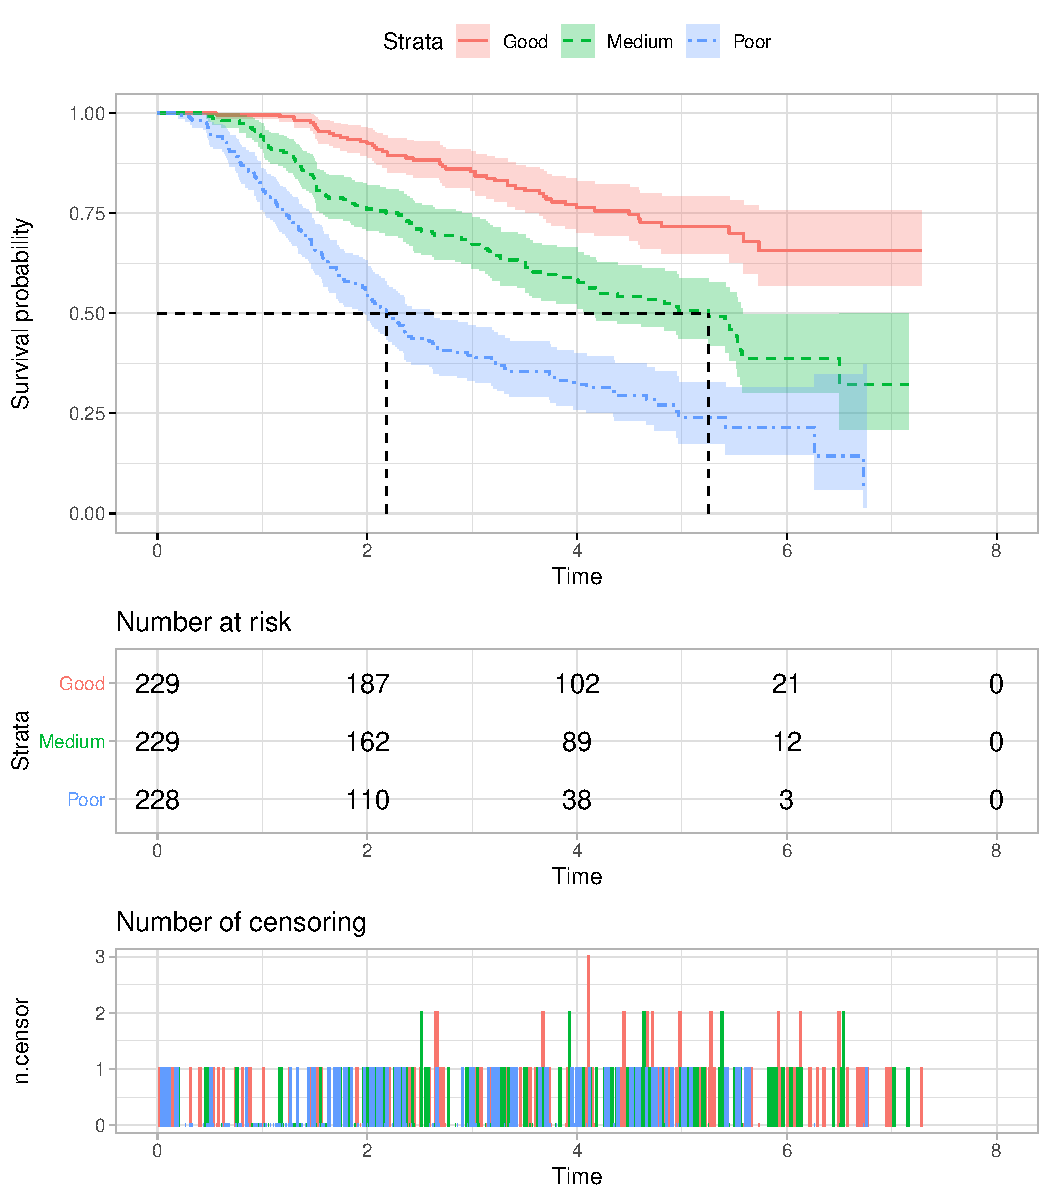
\includegraphics{images/plot_KM-1} \end{flushleft}

\newpage

\section{Stratified models?}\label{stratified-models}

Should stratified parametric survival models be used?

\begin{flushleft}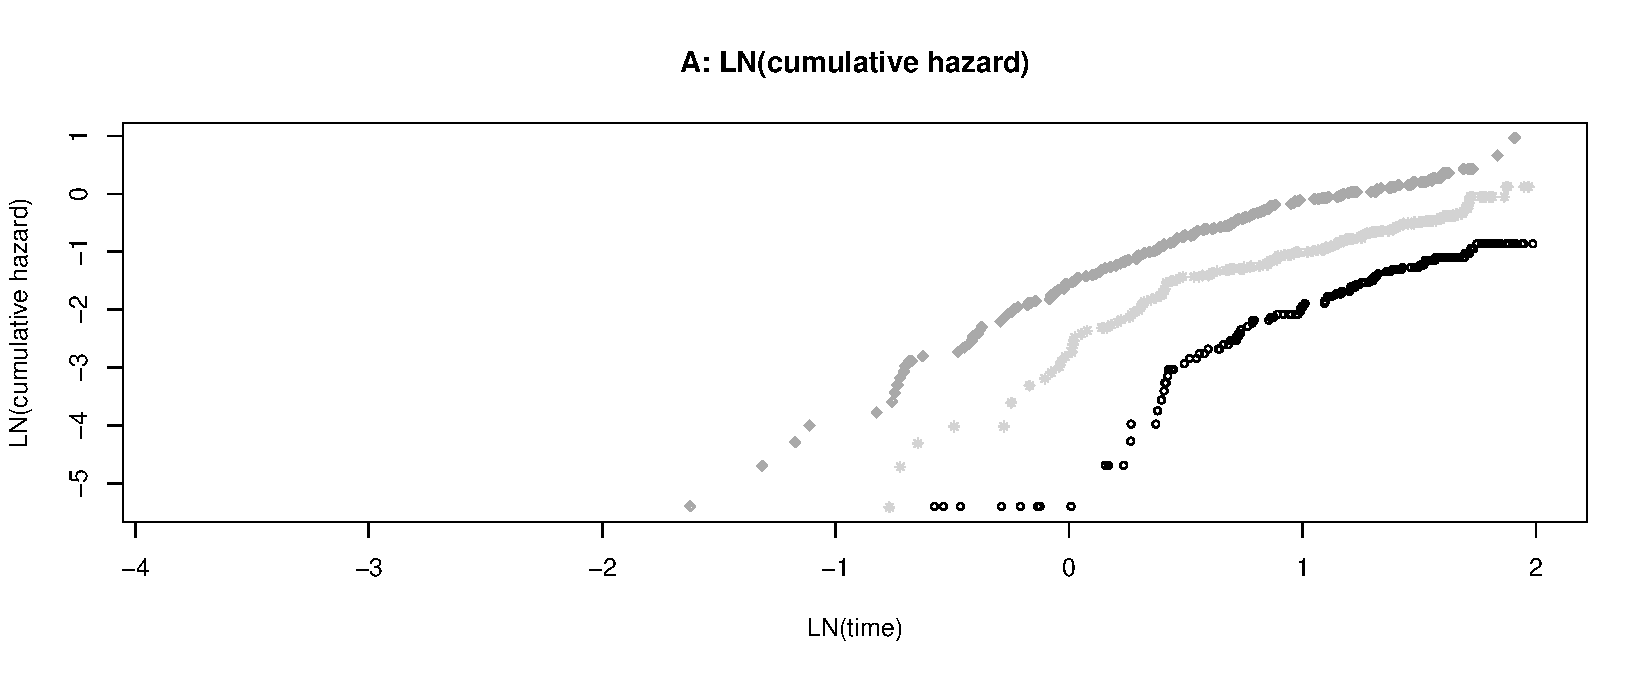
\includegraphics[height=0.29\textheight]{images/PH_assumption-1} \end{flushleft}

\begin{flushleft}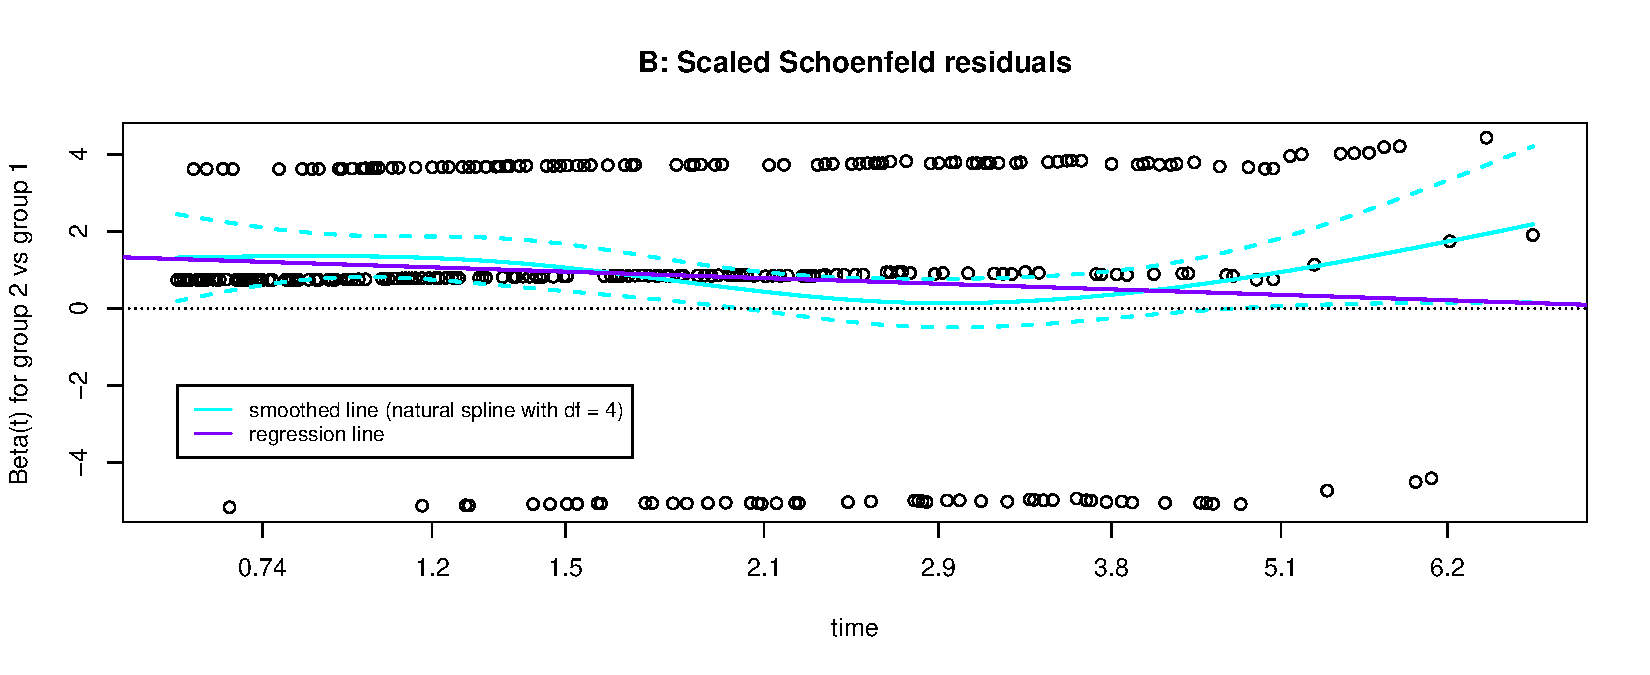
\includegraphics[height=0.29\textheight]{images/PH_assumption-2} \end{flushleft}

\begin{flushleft}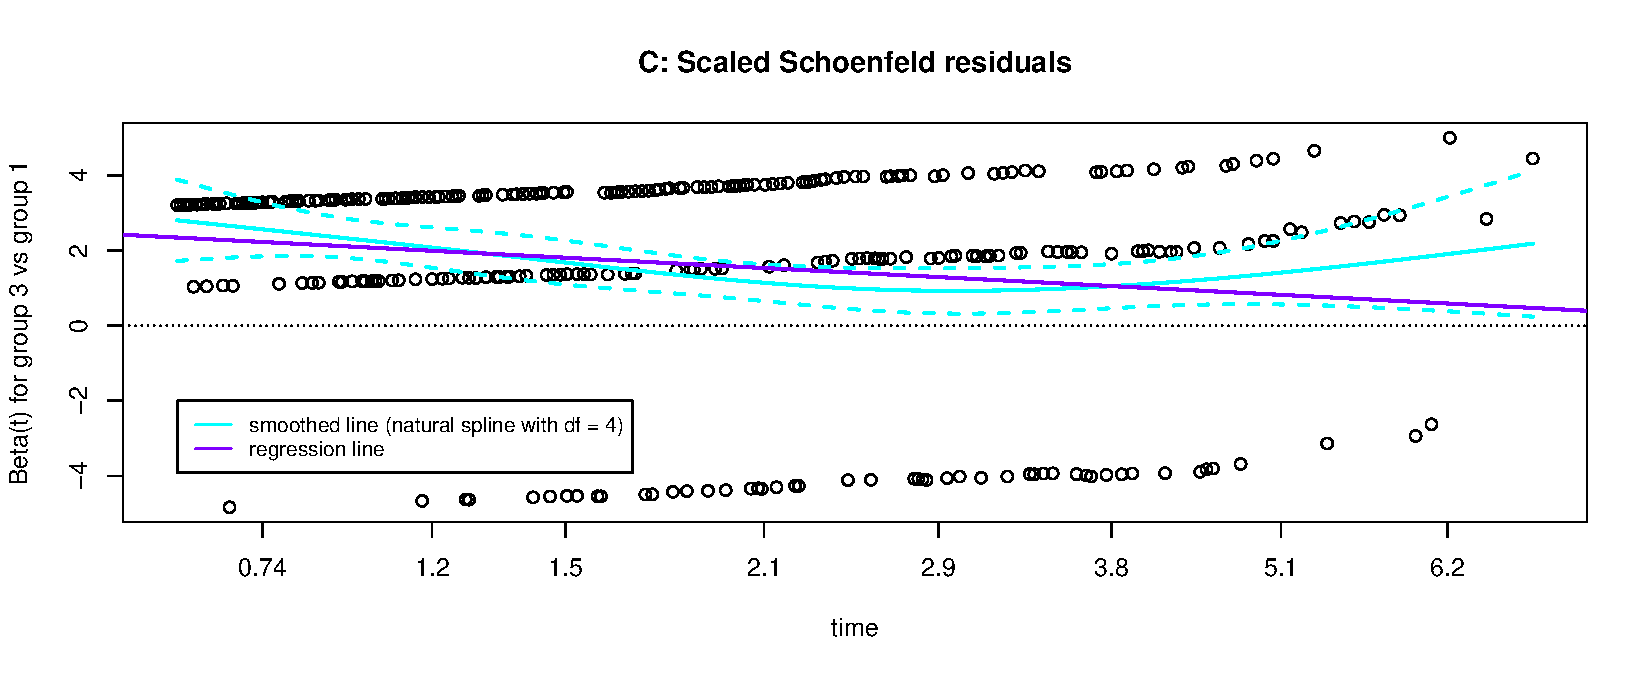
\includegraphics[height=0.29\textheight]{images/PH_assumption-3} \end{flushleft}

\newpage

\section{Monotonic hazard models?}\label{monotonic-hazard-models}

Should parametric survival models assuming a monotonic hazard rate
(i.e.~exponential, Weibull, Gompertz) be used?

\begin{flushleft}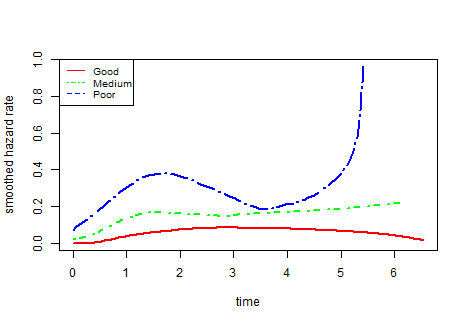
\includegraphics{images/plot_hr-1} \end{flushleft}

\newpage

\section{Standard parametric models?}\label{standard-parametric-models}

Do standard parametric models provide an appropriate fit to the data?

\begin{flushleft}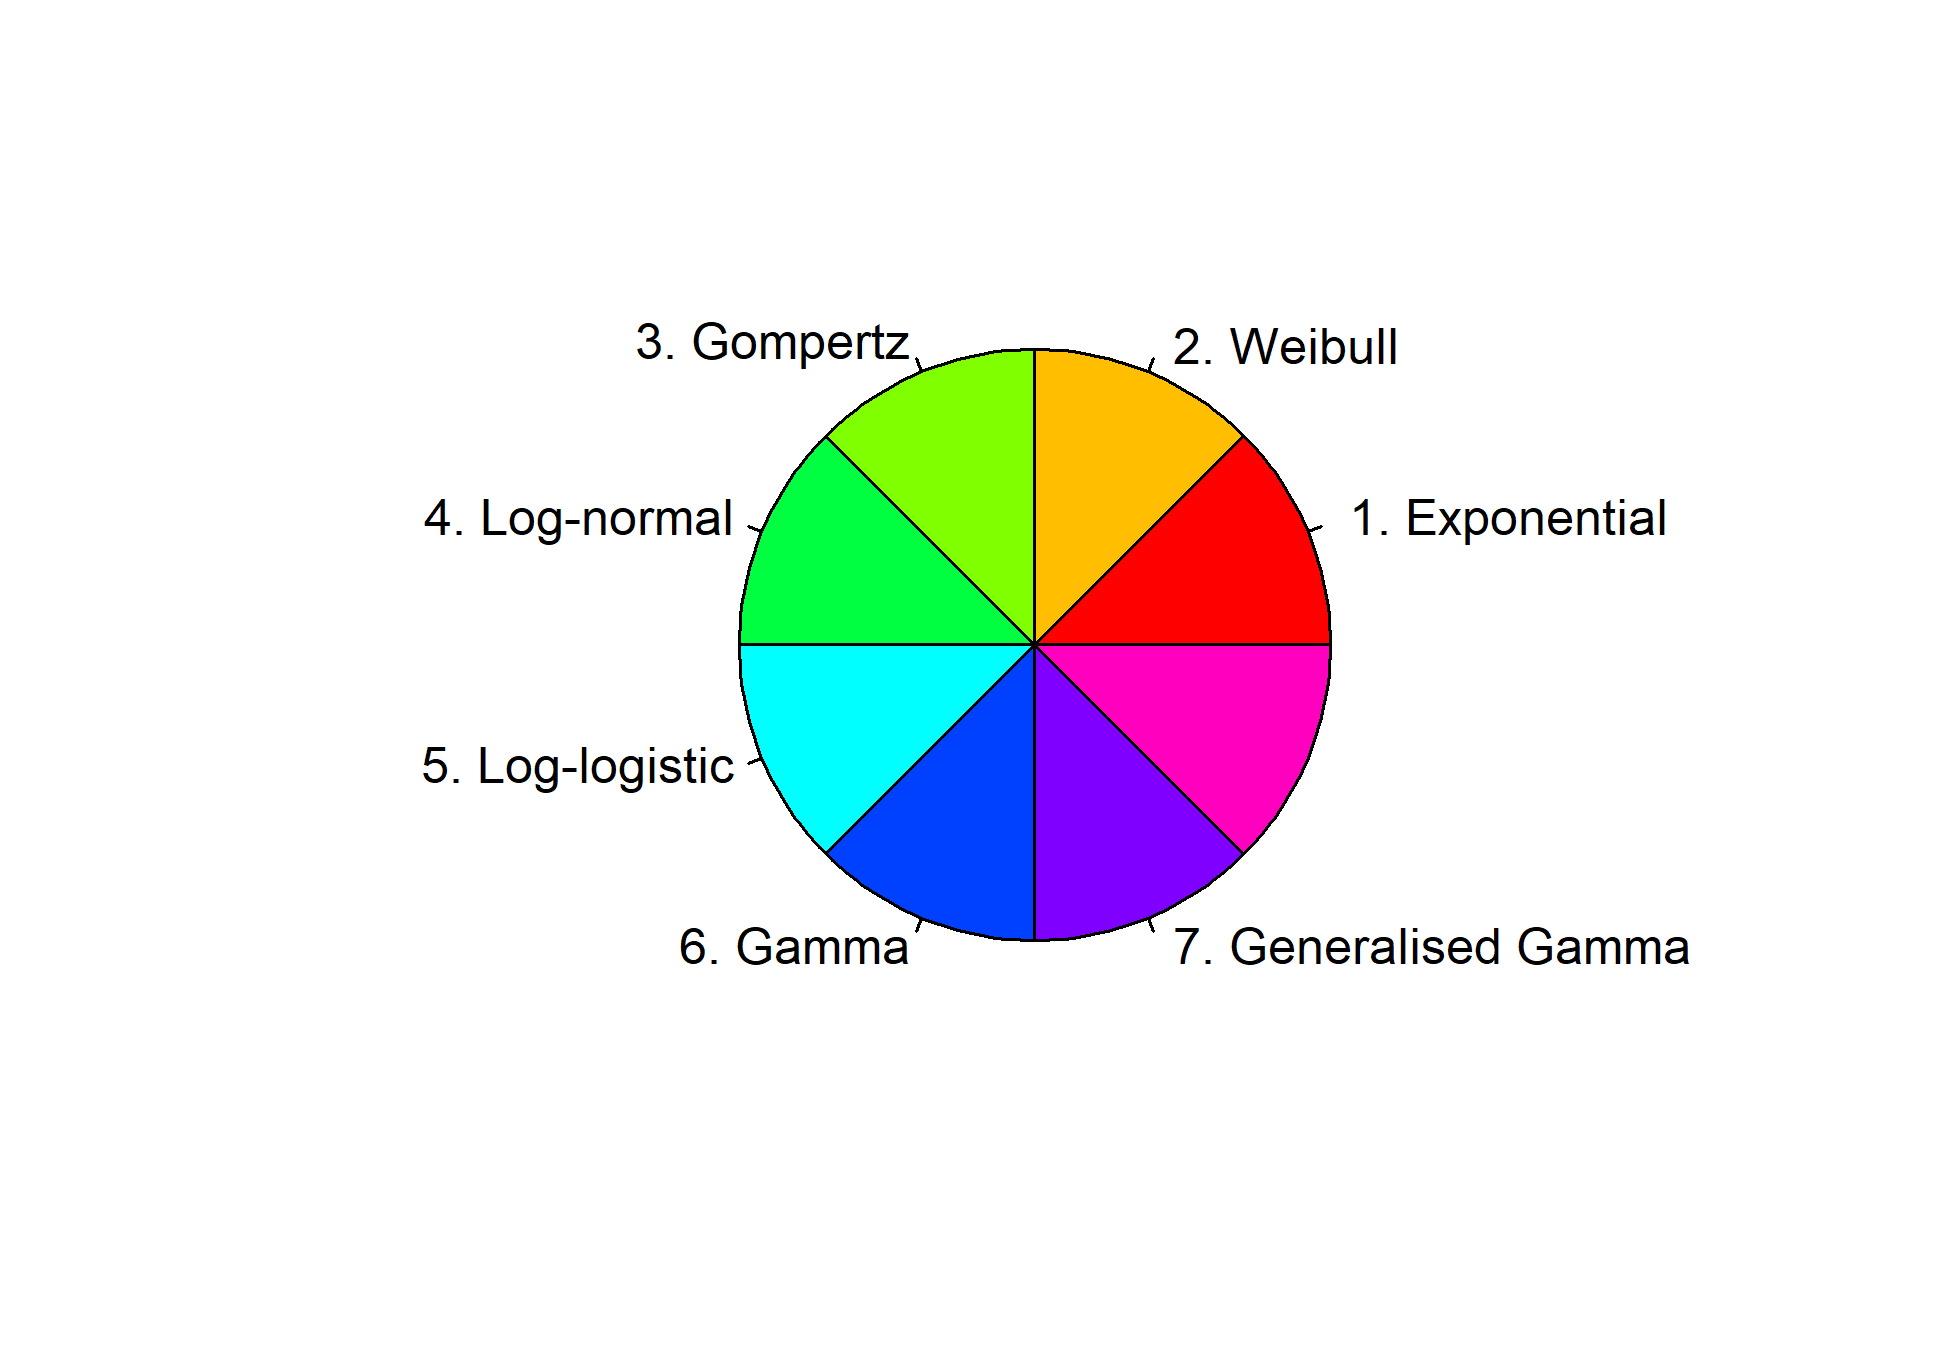
\includegraphics{images/plot_parametric-1} \end{flushleft}

\begin{table}[H]
\centering
\begin{tabular}{lrr}
\toprule
Model & AIC & BIC\\
\midrule
\rowcolor{gray!6}  7. Generalised Gamma & 1589.049 & 1629.826\\
4. Log-normal & 1592.880 & 1620.066\\
\rowcolor{gray!6}  5. Log-logistic & 1609.294 & 1636.479\\
6. Gamma & 1621.982 & 1649.167\\
\rowcolor{gray!6}  2. Weibull & 1632.618 & 1659.803\\
3. Gompertz & 1660.954 & 1688.140\\
\rowcolor{gray!6}  1. Exponential & 1668.212 & 1681.805\\
\bottomrule
\end{tabular}
\end{table}

\subsection{Exponential}\label{exponential}

\begin{flushleft}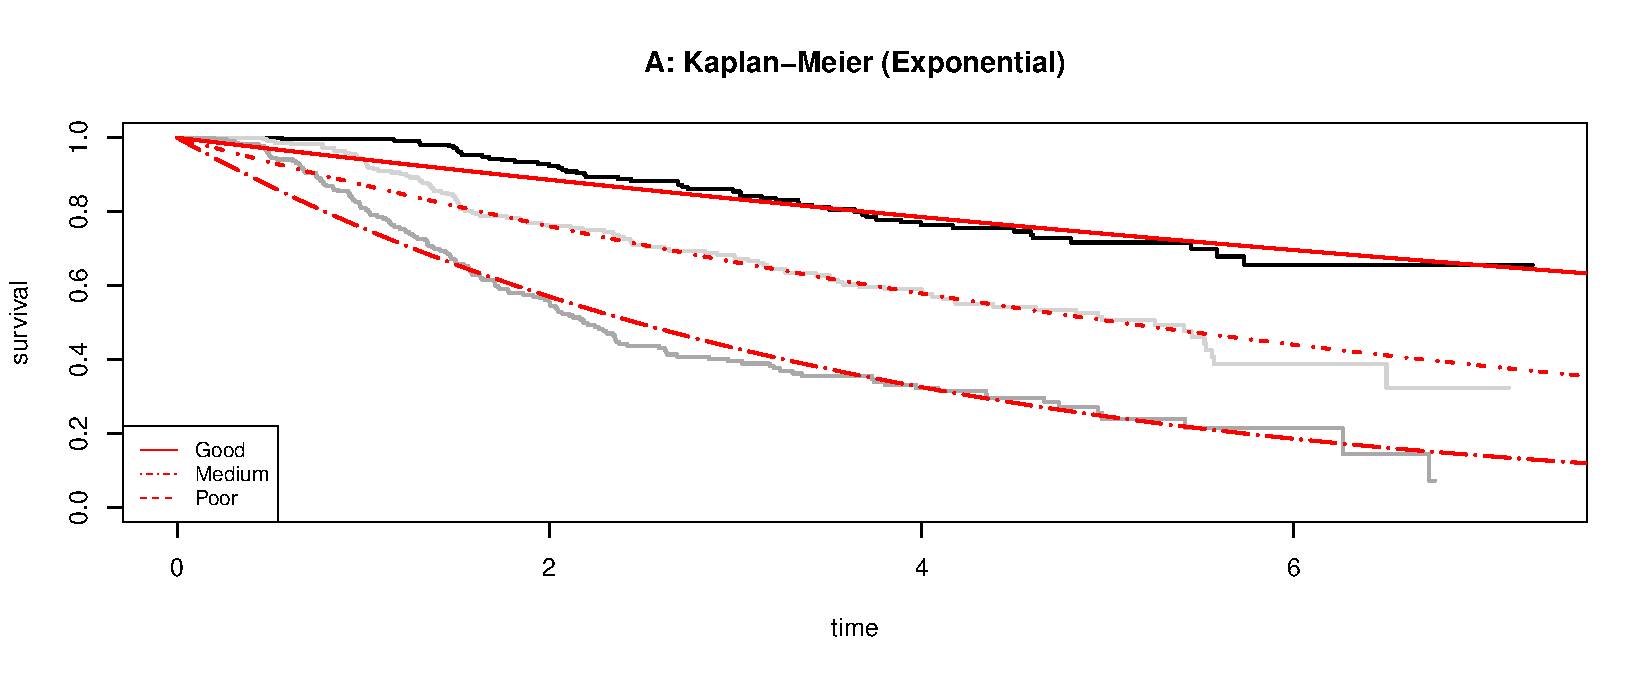
\includegraphics[height=0.3\textheight]{images/expo-1} \end{flushleft}

\begin{flushleft}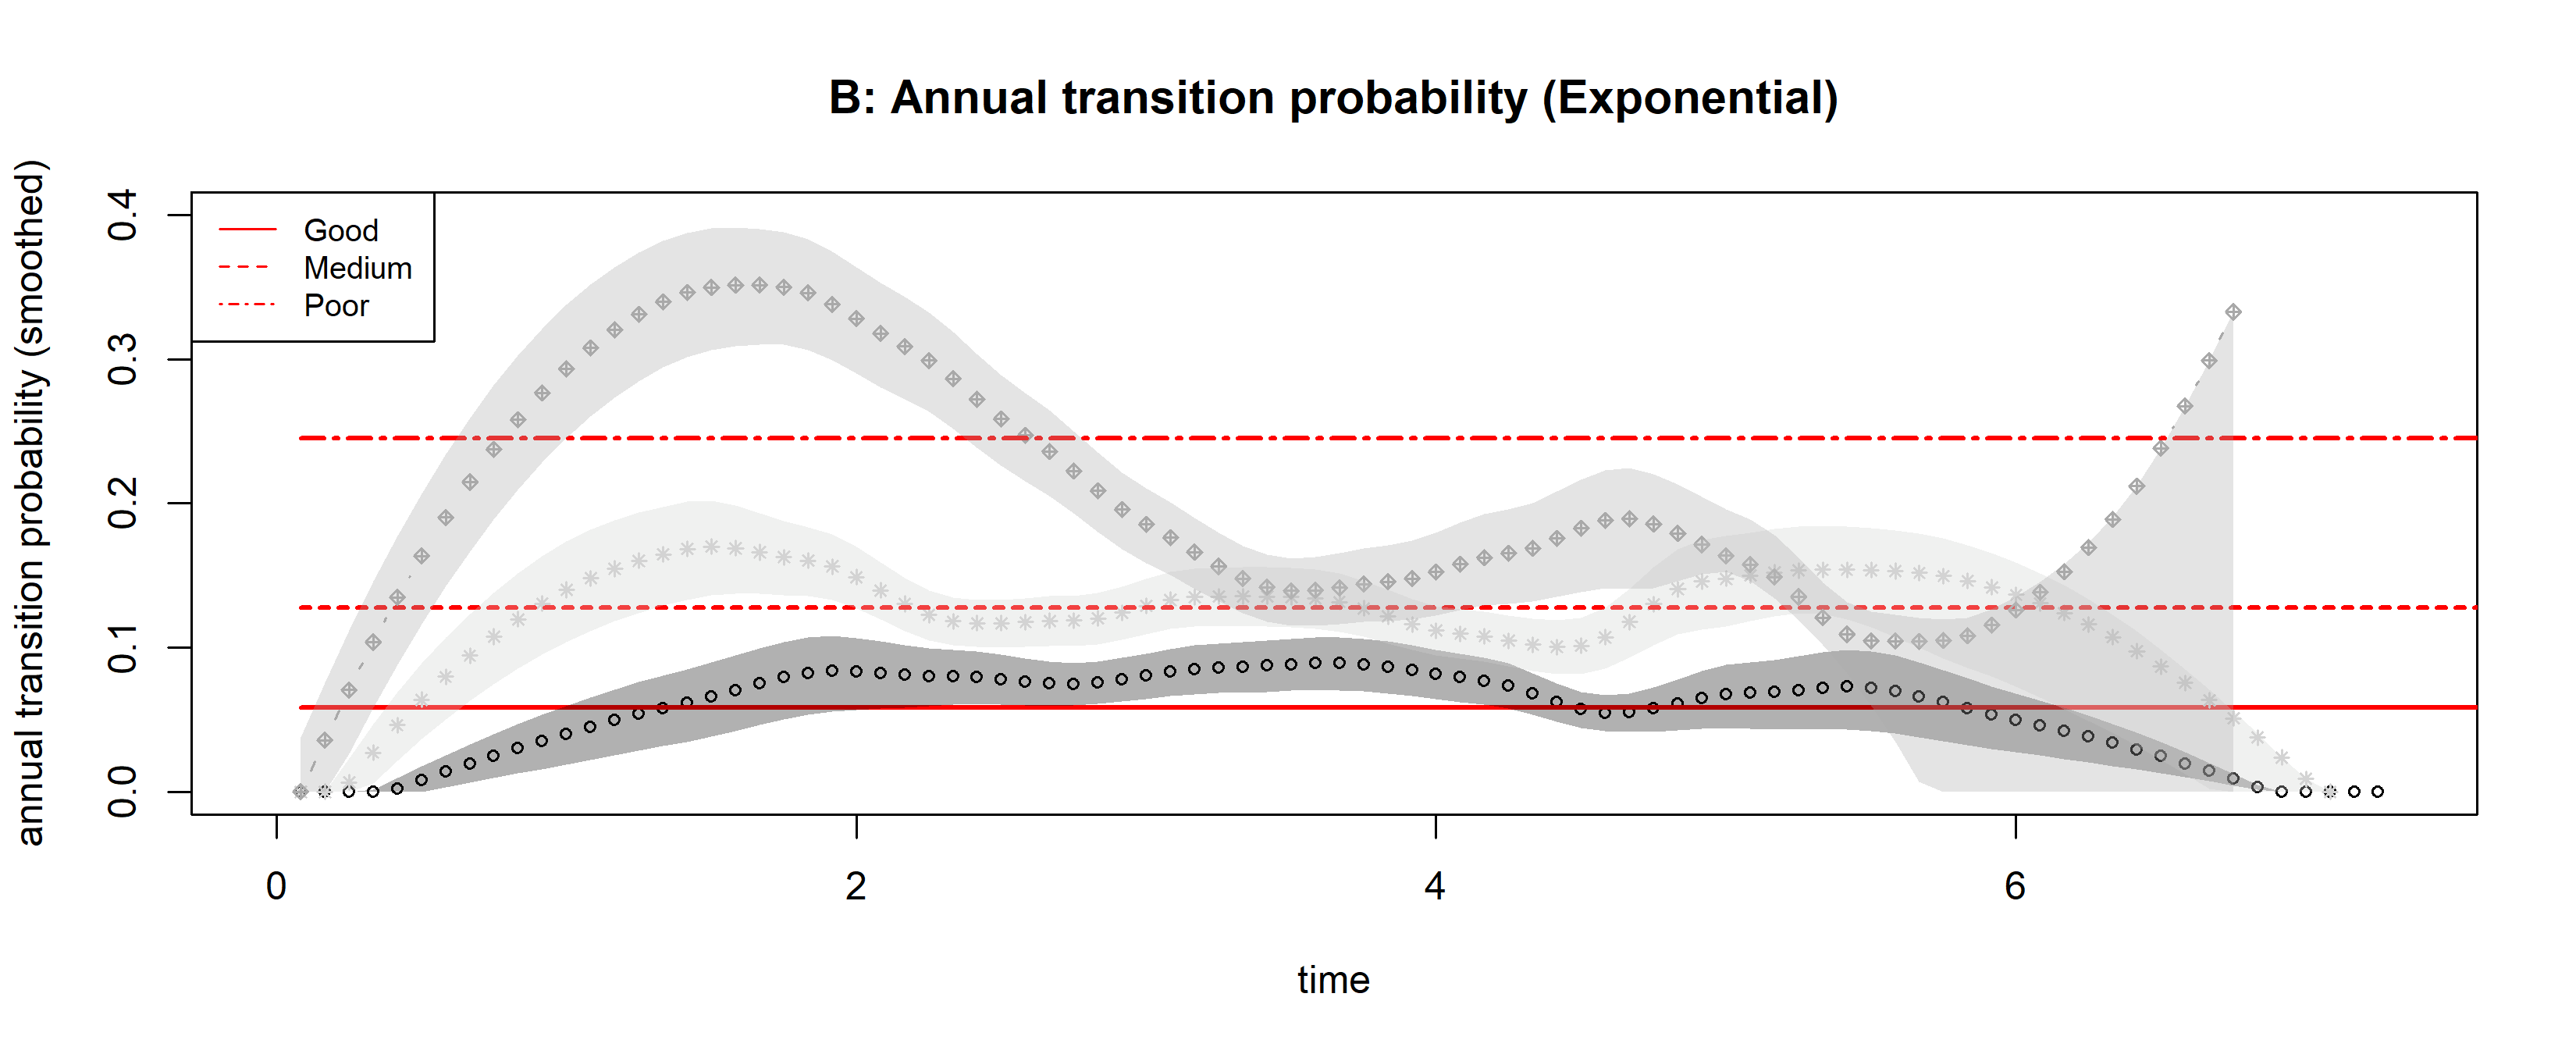
\includegraphics[height=0.3\textheight]{images/expo-2} \end{flushleft}

\begin{flushleft}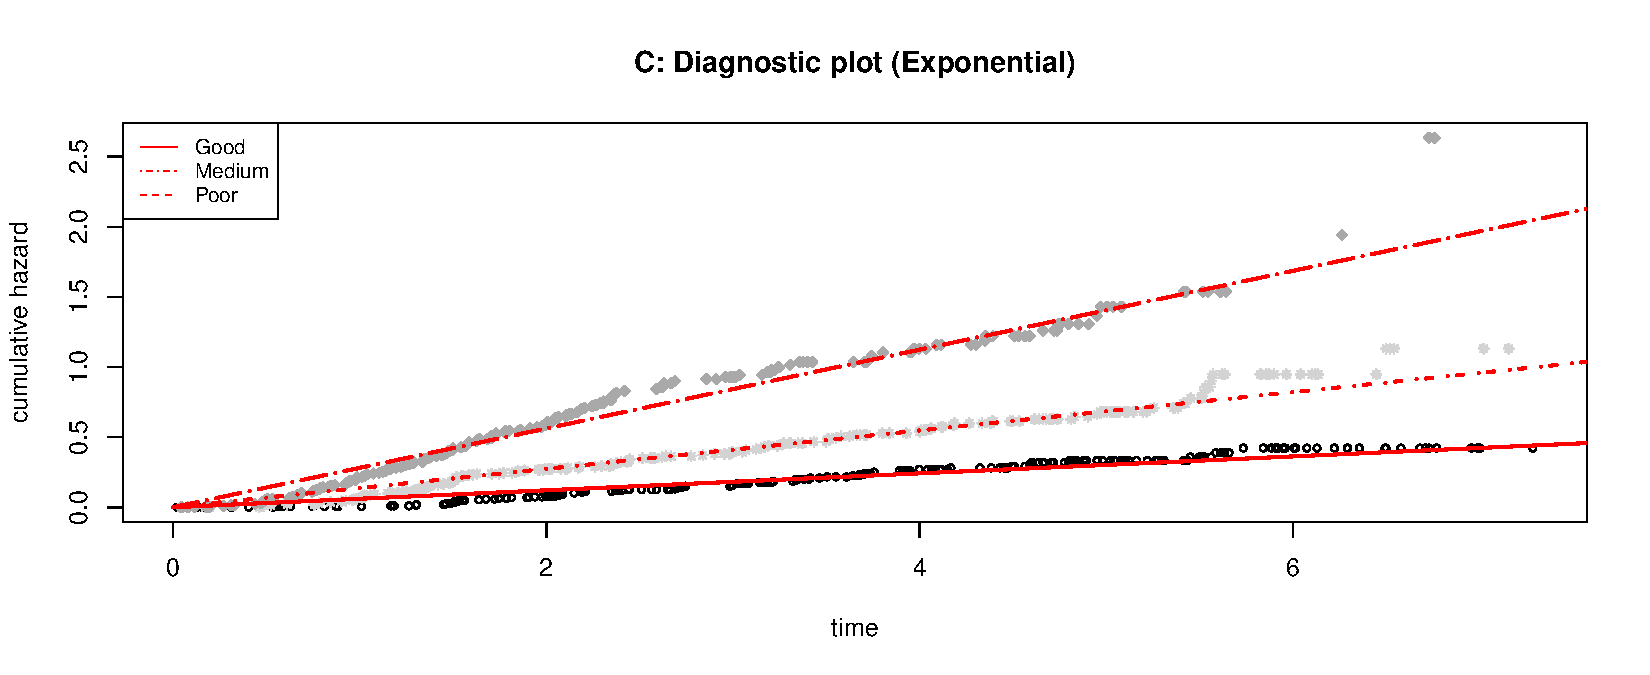
\includegraphics[height=0.3\textheight]{images/expo-3} \end{flushleft}

\subsection{Weibull}\label{weibull}

\begin{flushleft}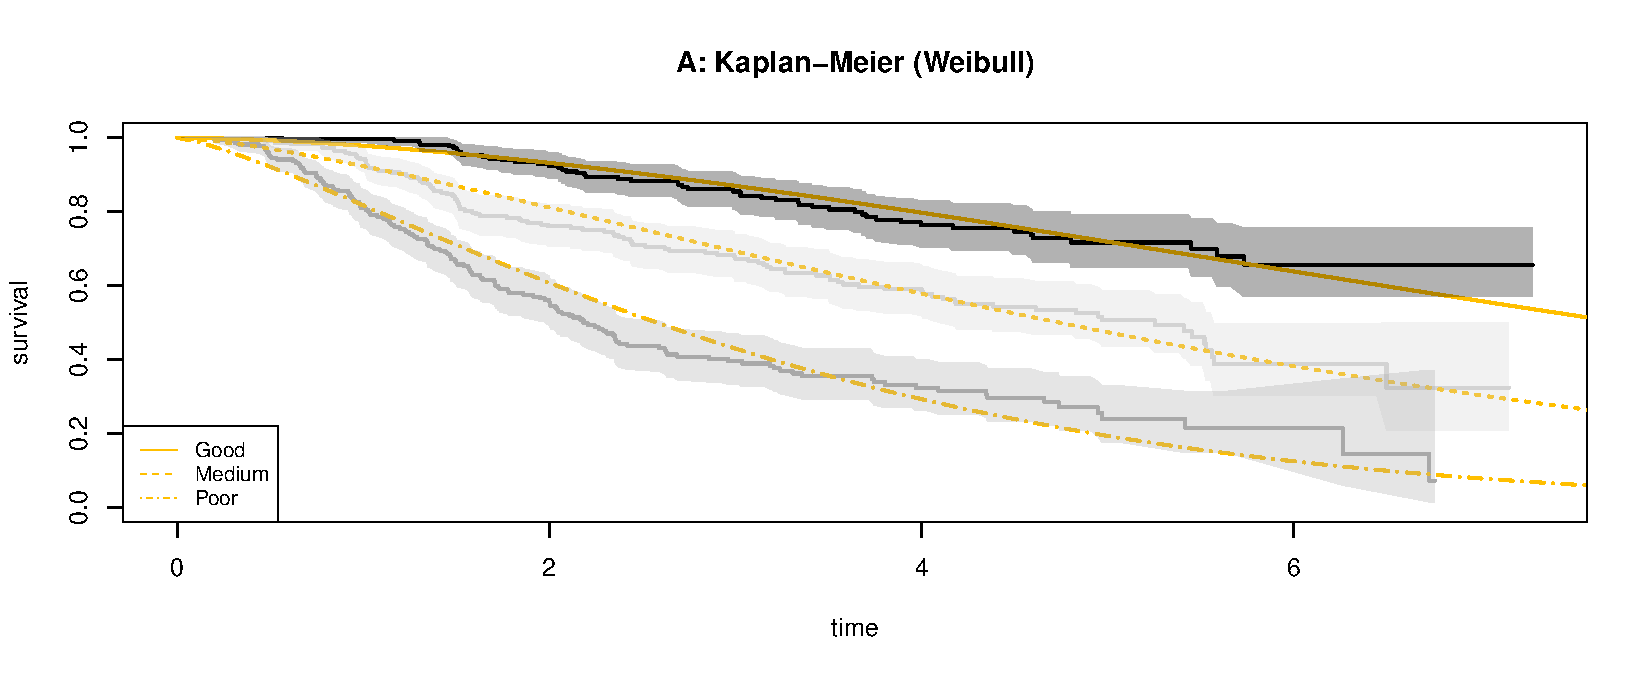
\includegraphics[height=0.3\textheight]{images/weib-1} \end{flushleft}

\begin{flushleft}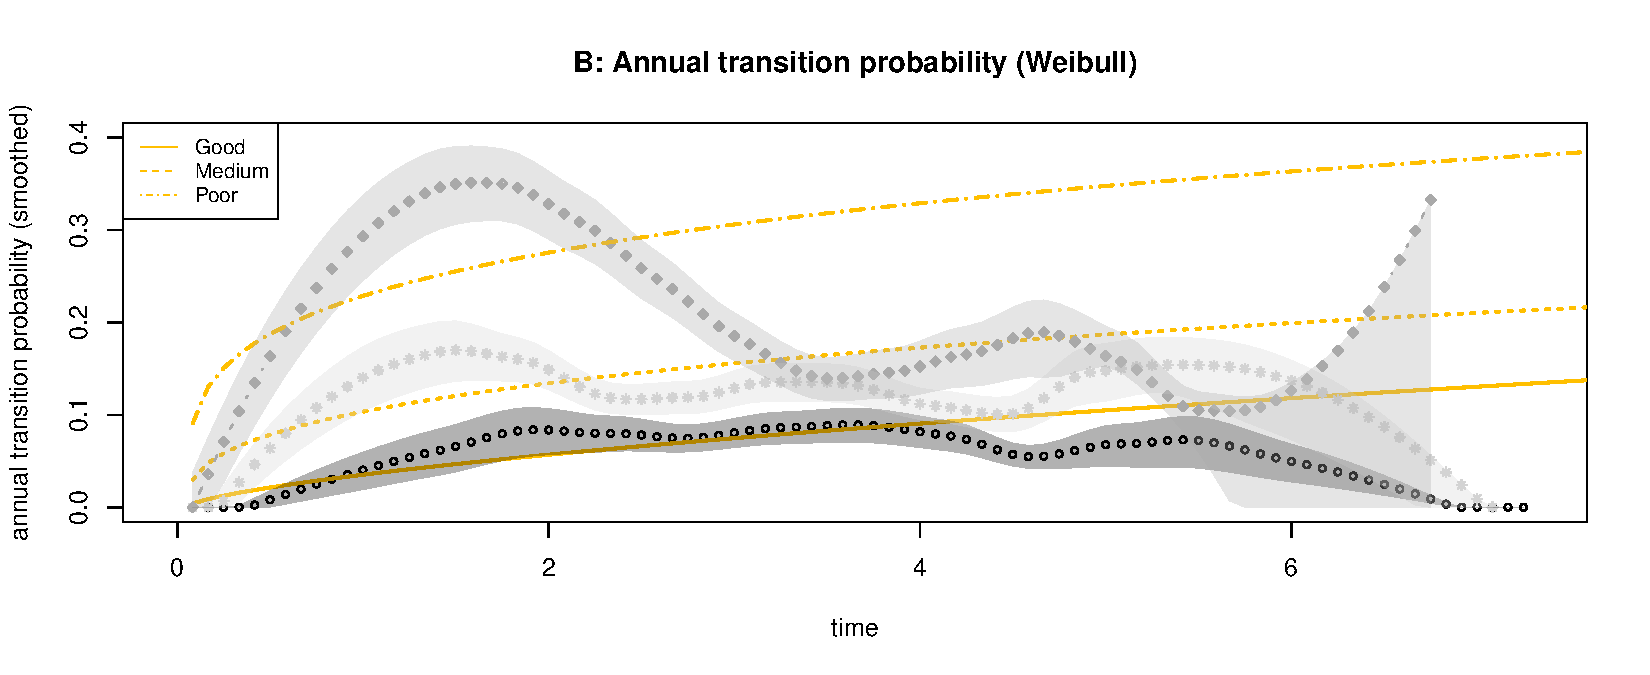
\includegraphics[height=0.3\textheight]{images/weib-2} \end{flushleft}

\begin{flushleft}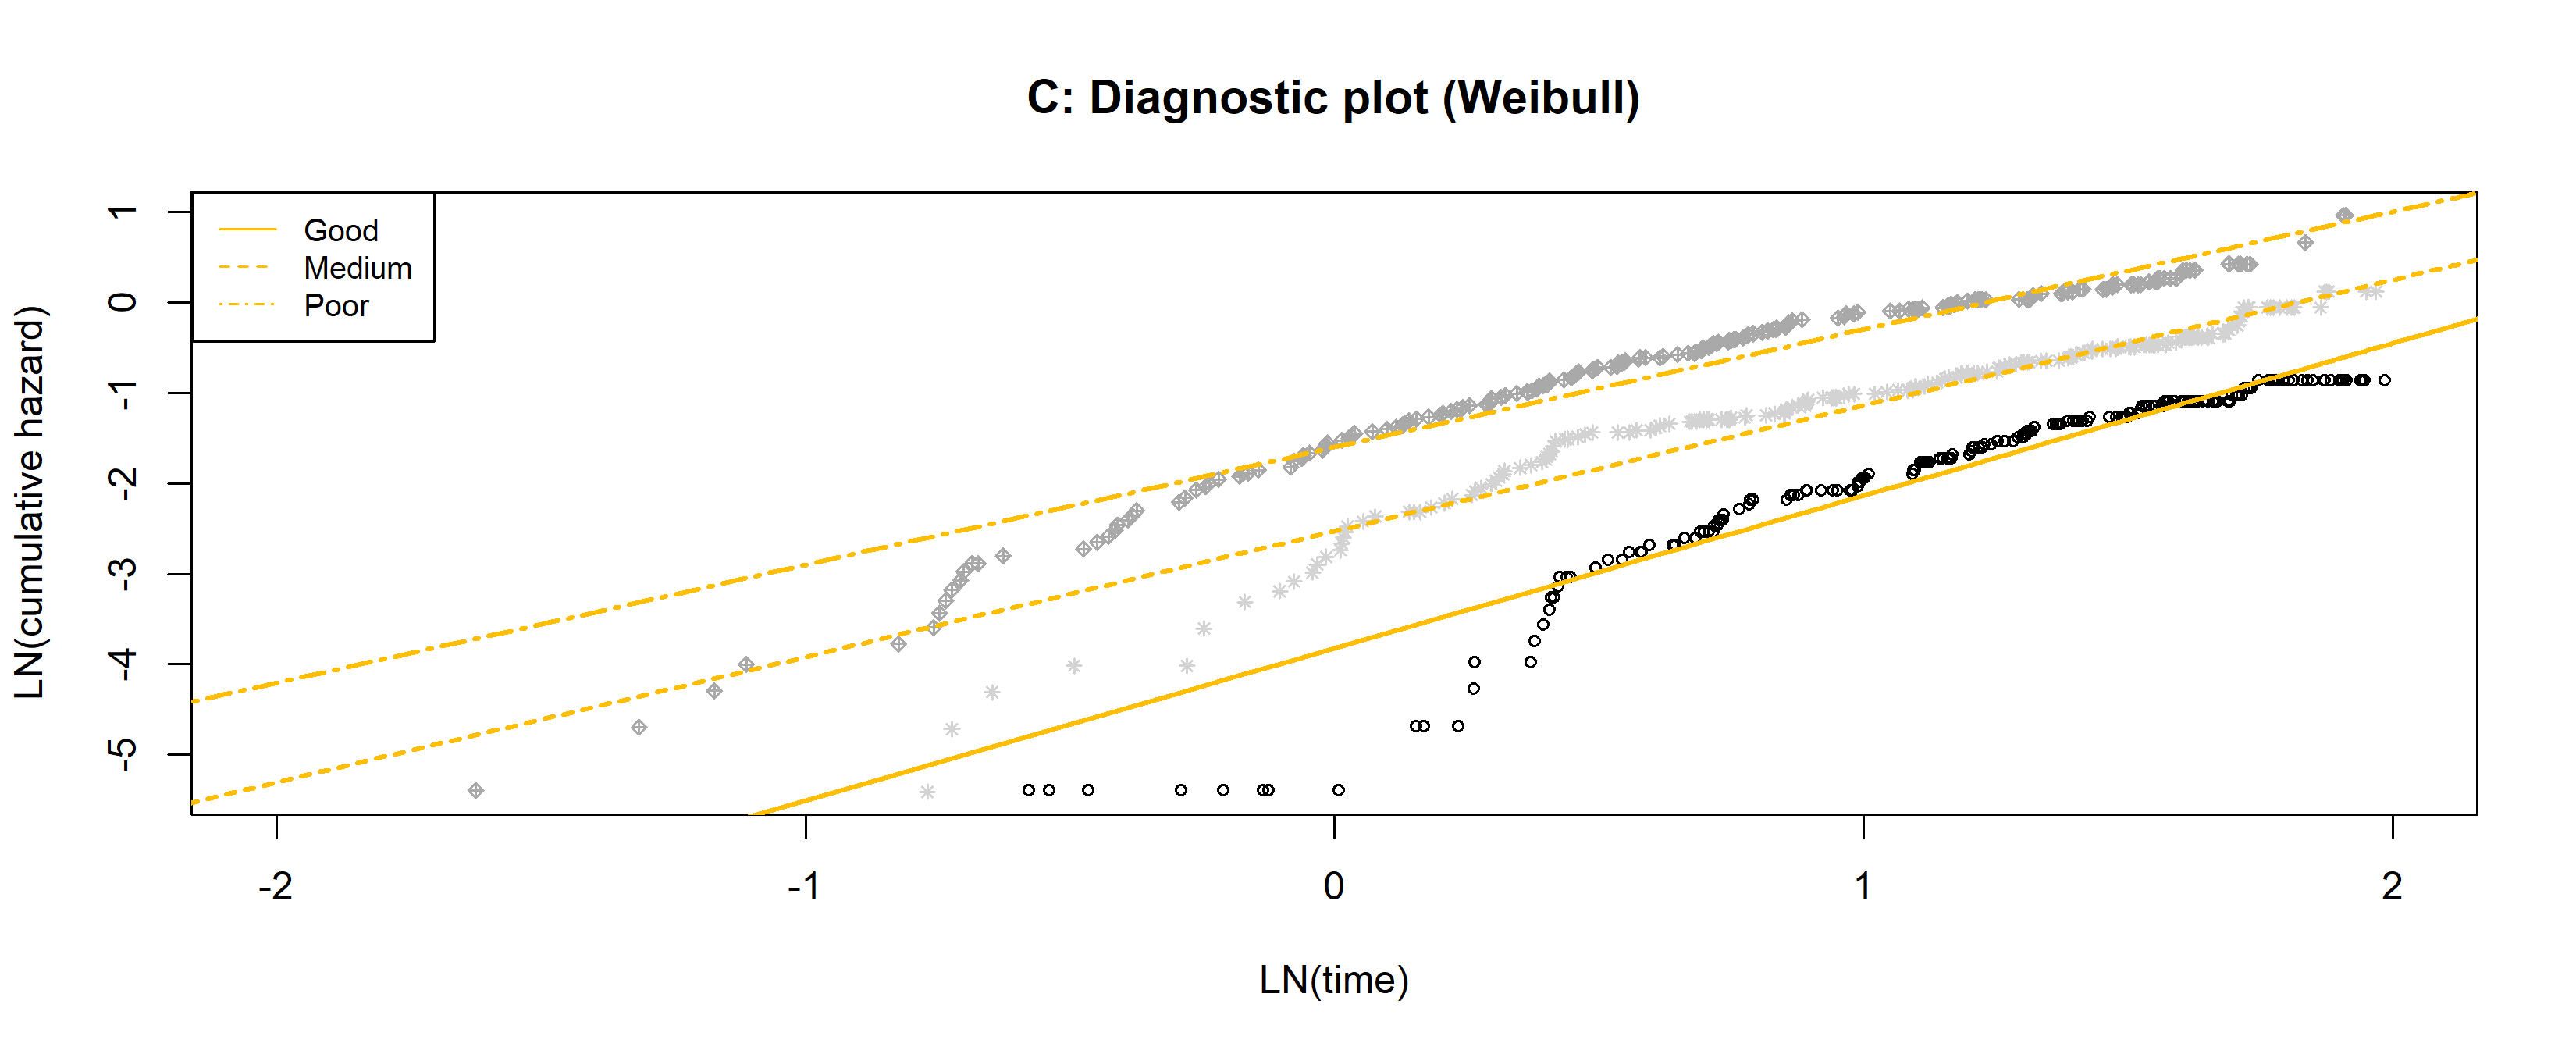
\includegraphics[height=0.3\textheight]{images/weib-3} \end{flushleft}

\subsection{Gompertz}\label{gompertz}

\begin{flushleft}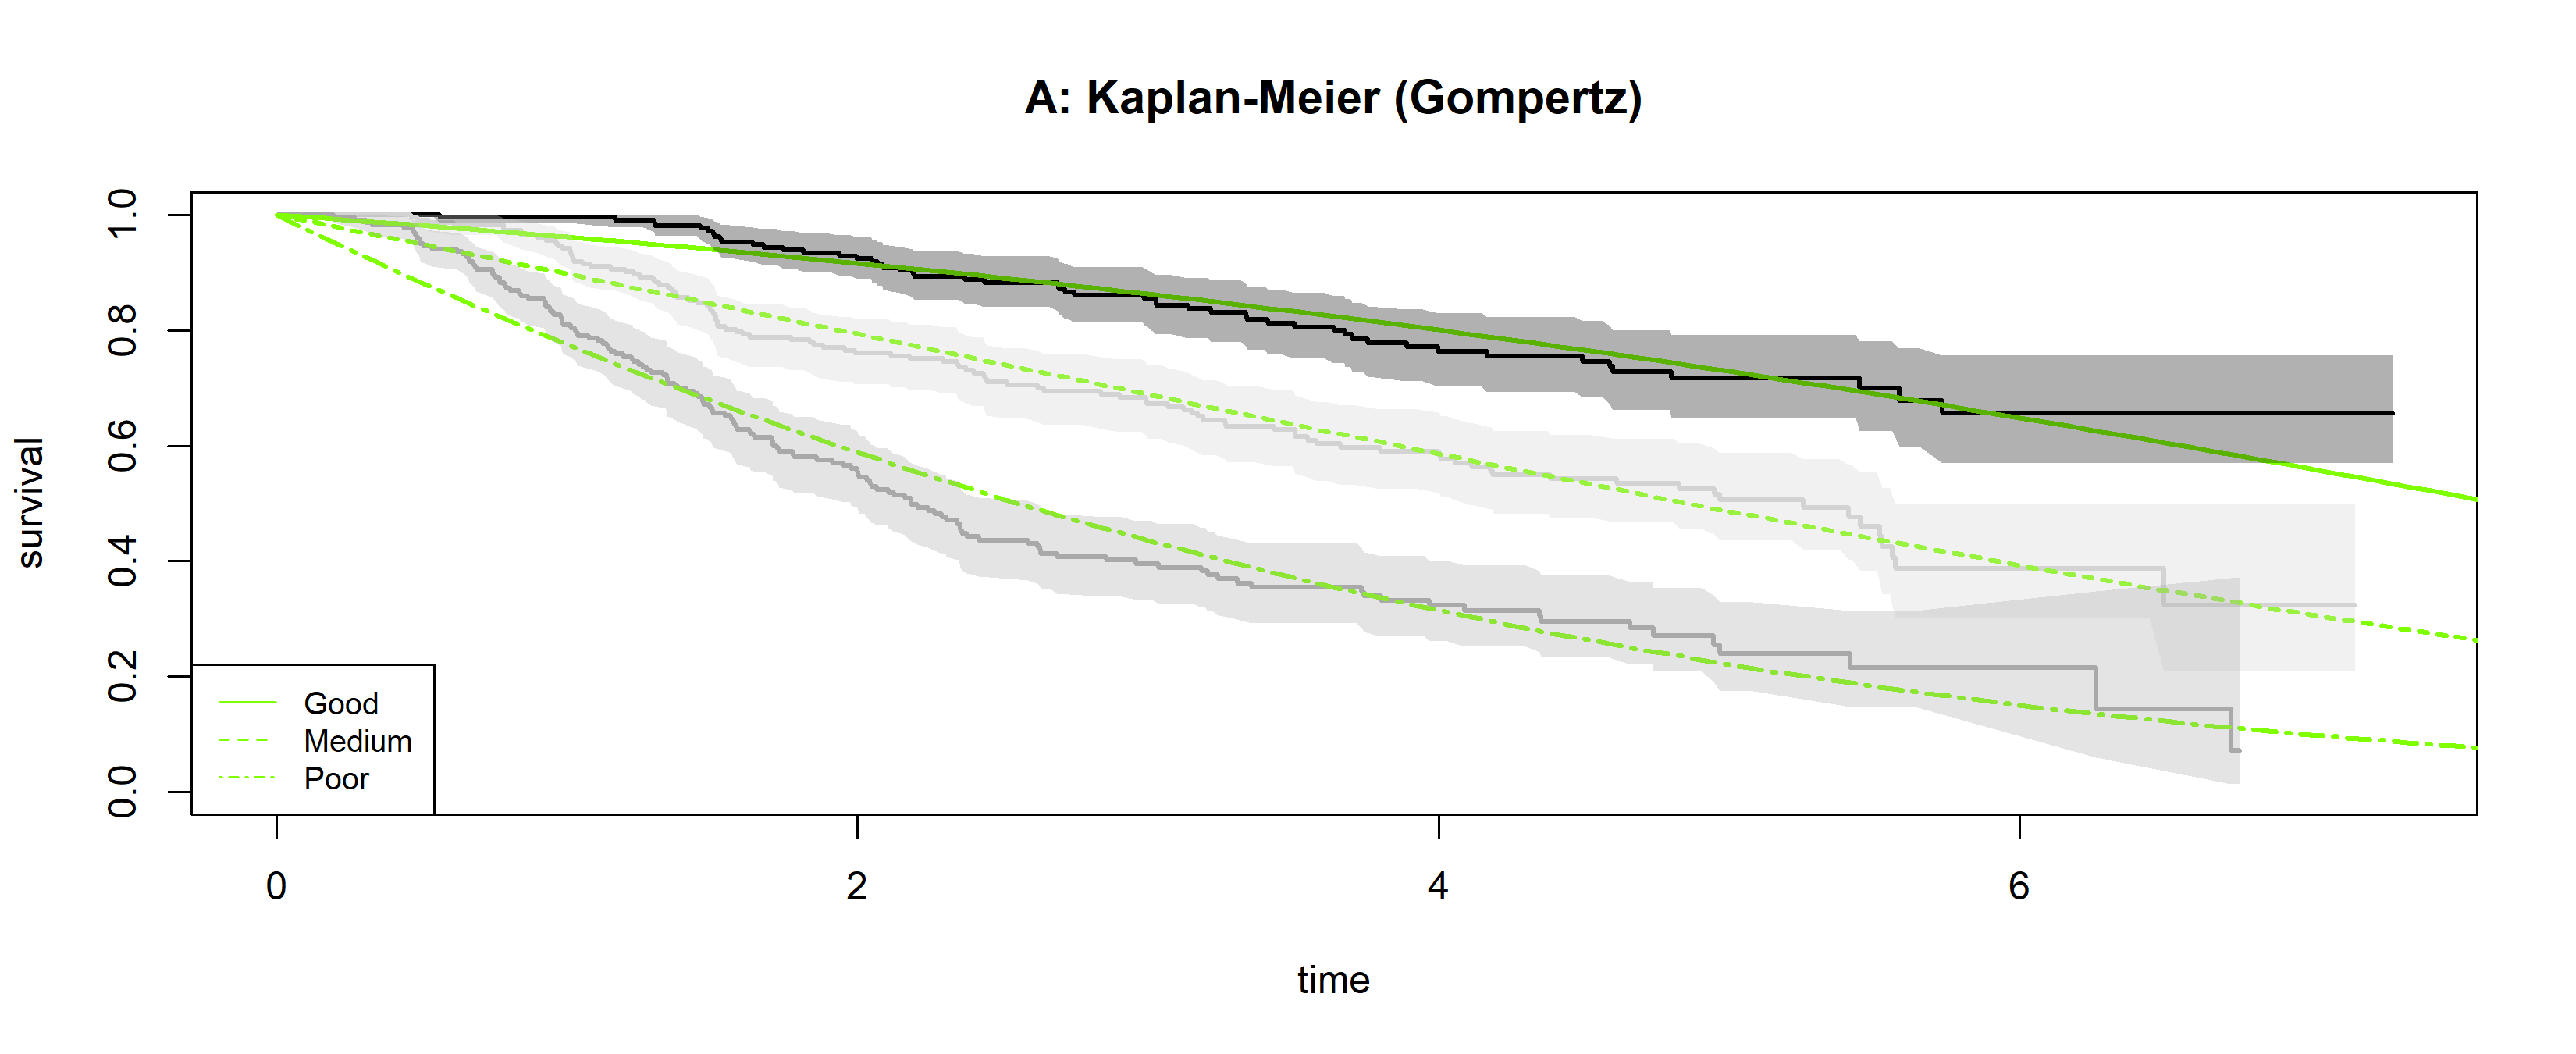
\includegraphics[height=0.3\textheight]{images/gom-1} \end{flushleft}

\begin{flushleft}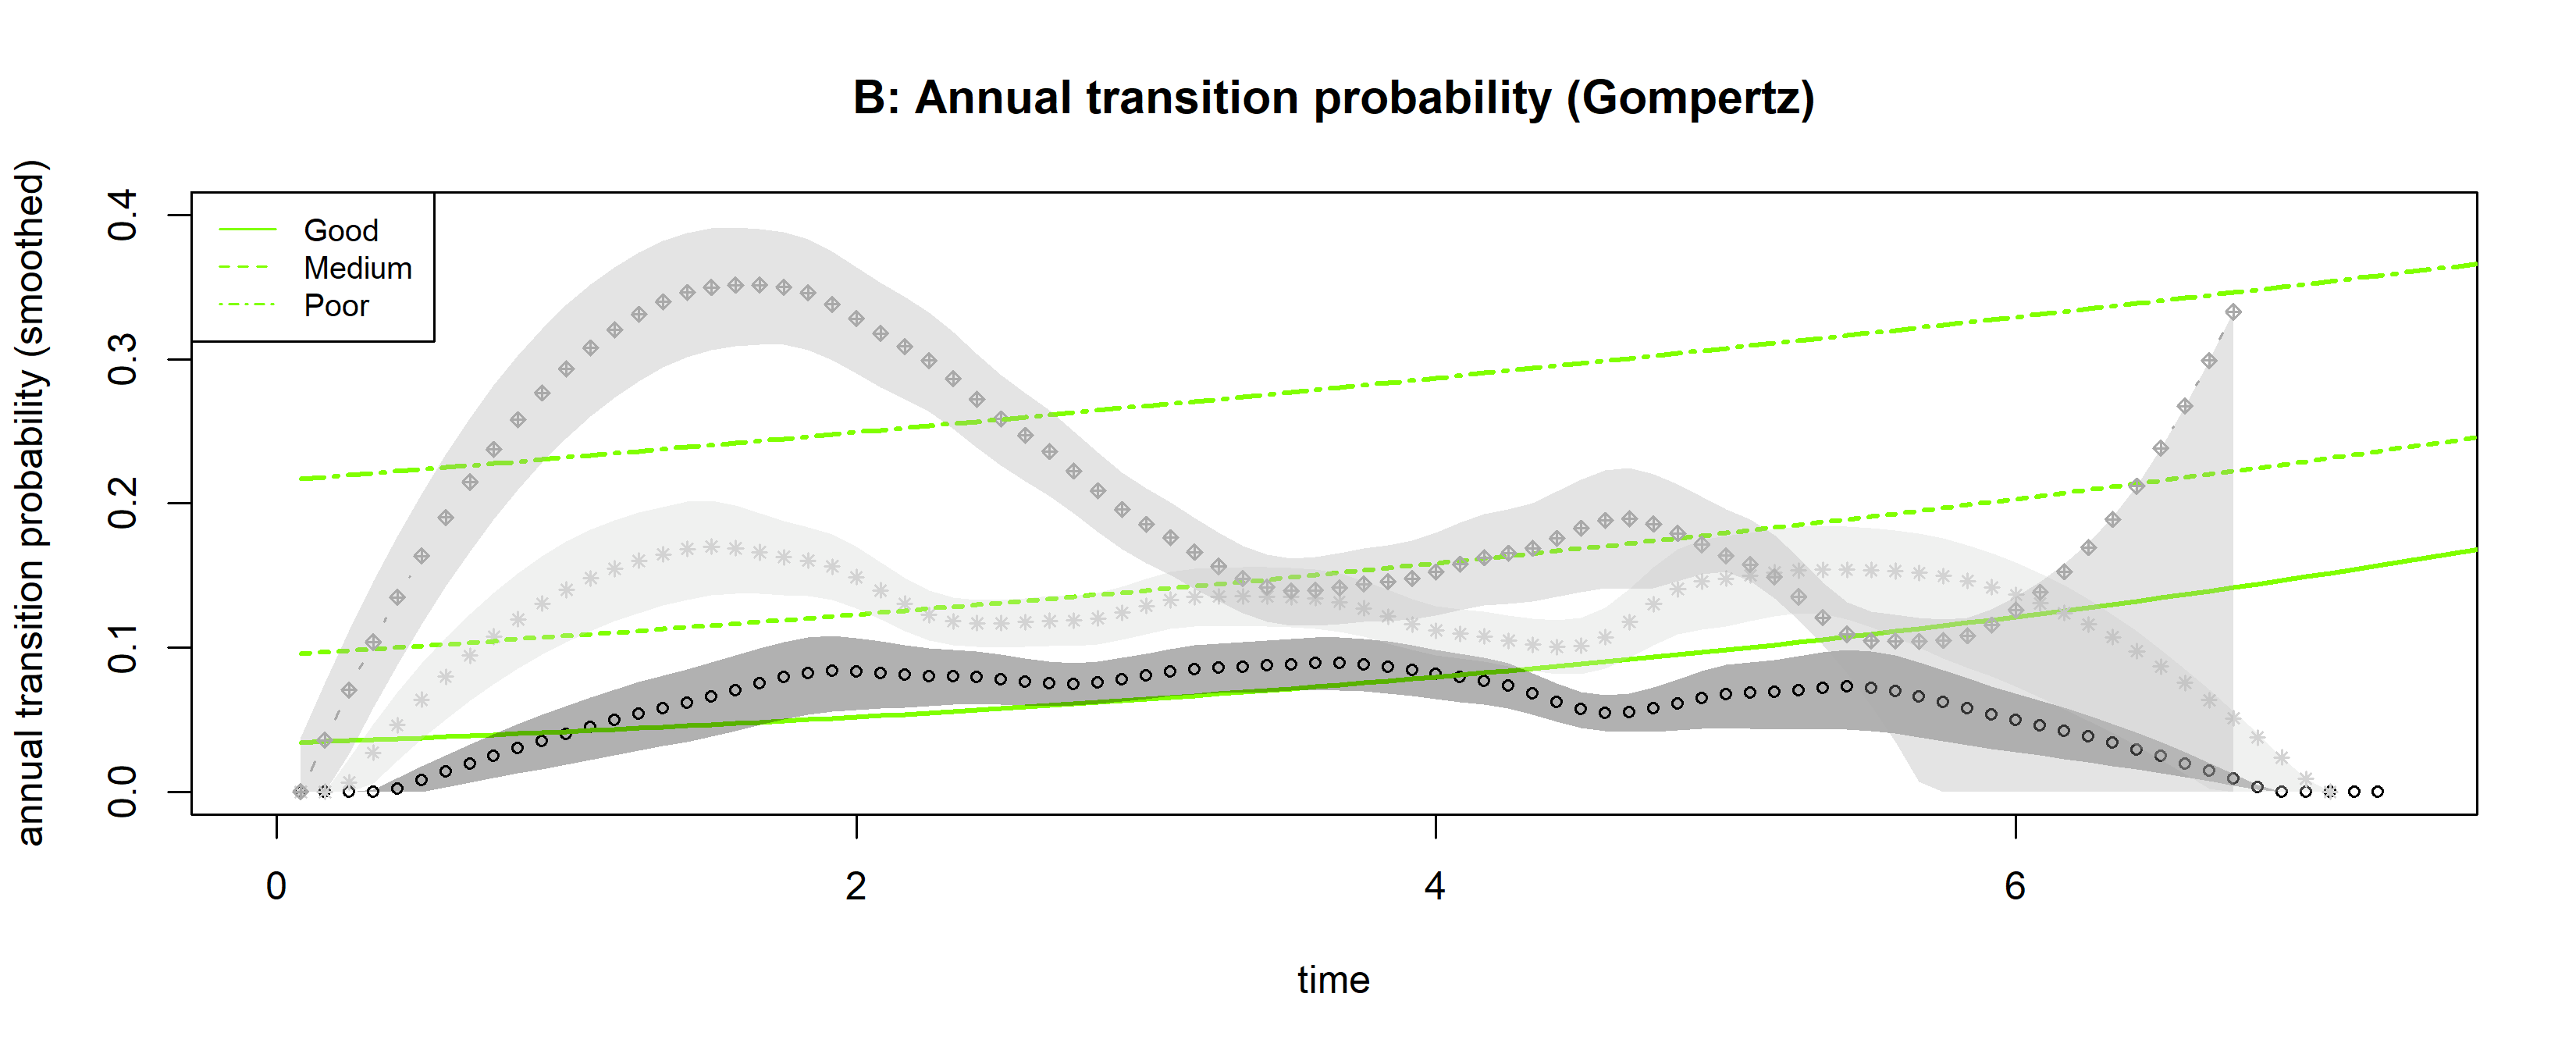
\includegraphics[height=0.3\textheight]{images/gom-2} \end{flushleft}

\begin{flushleft}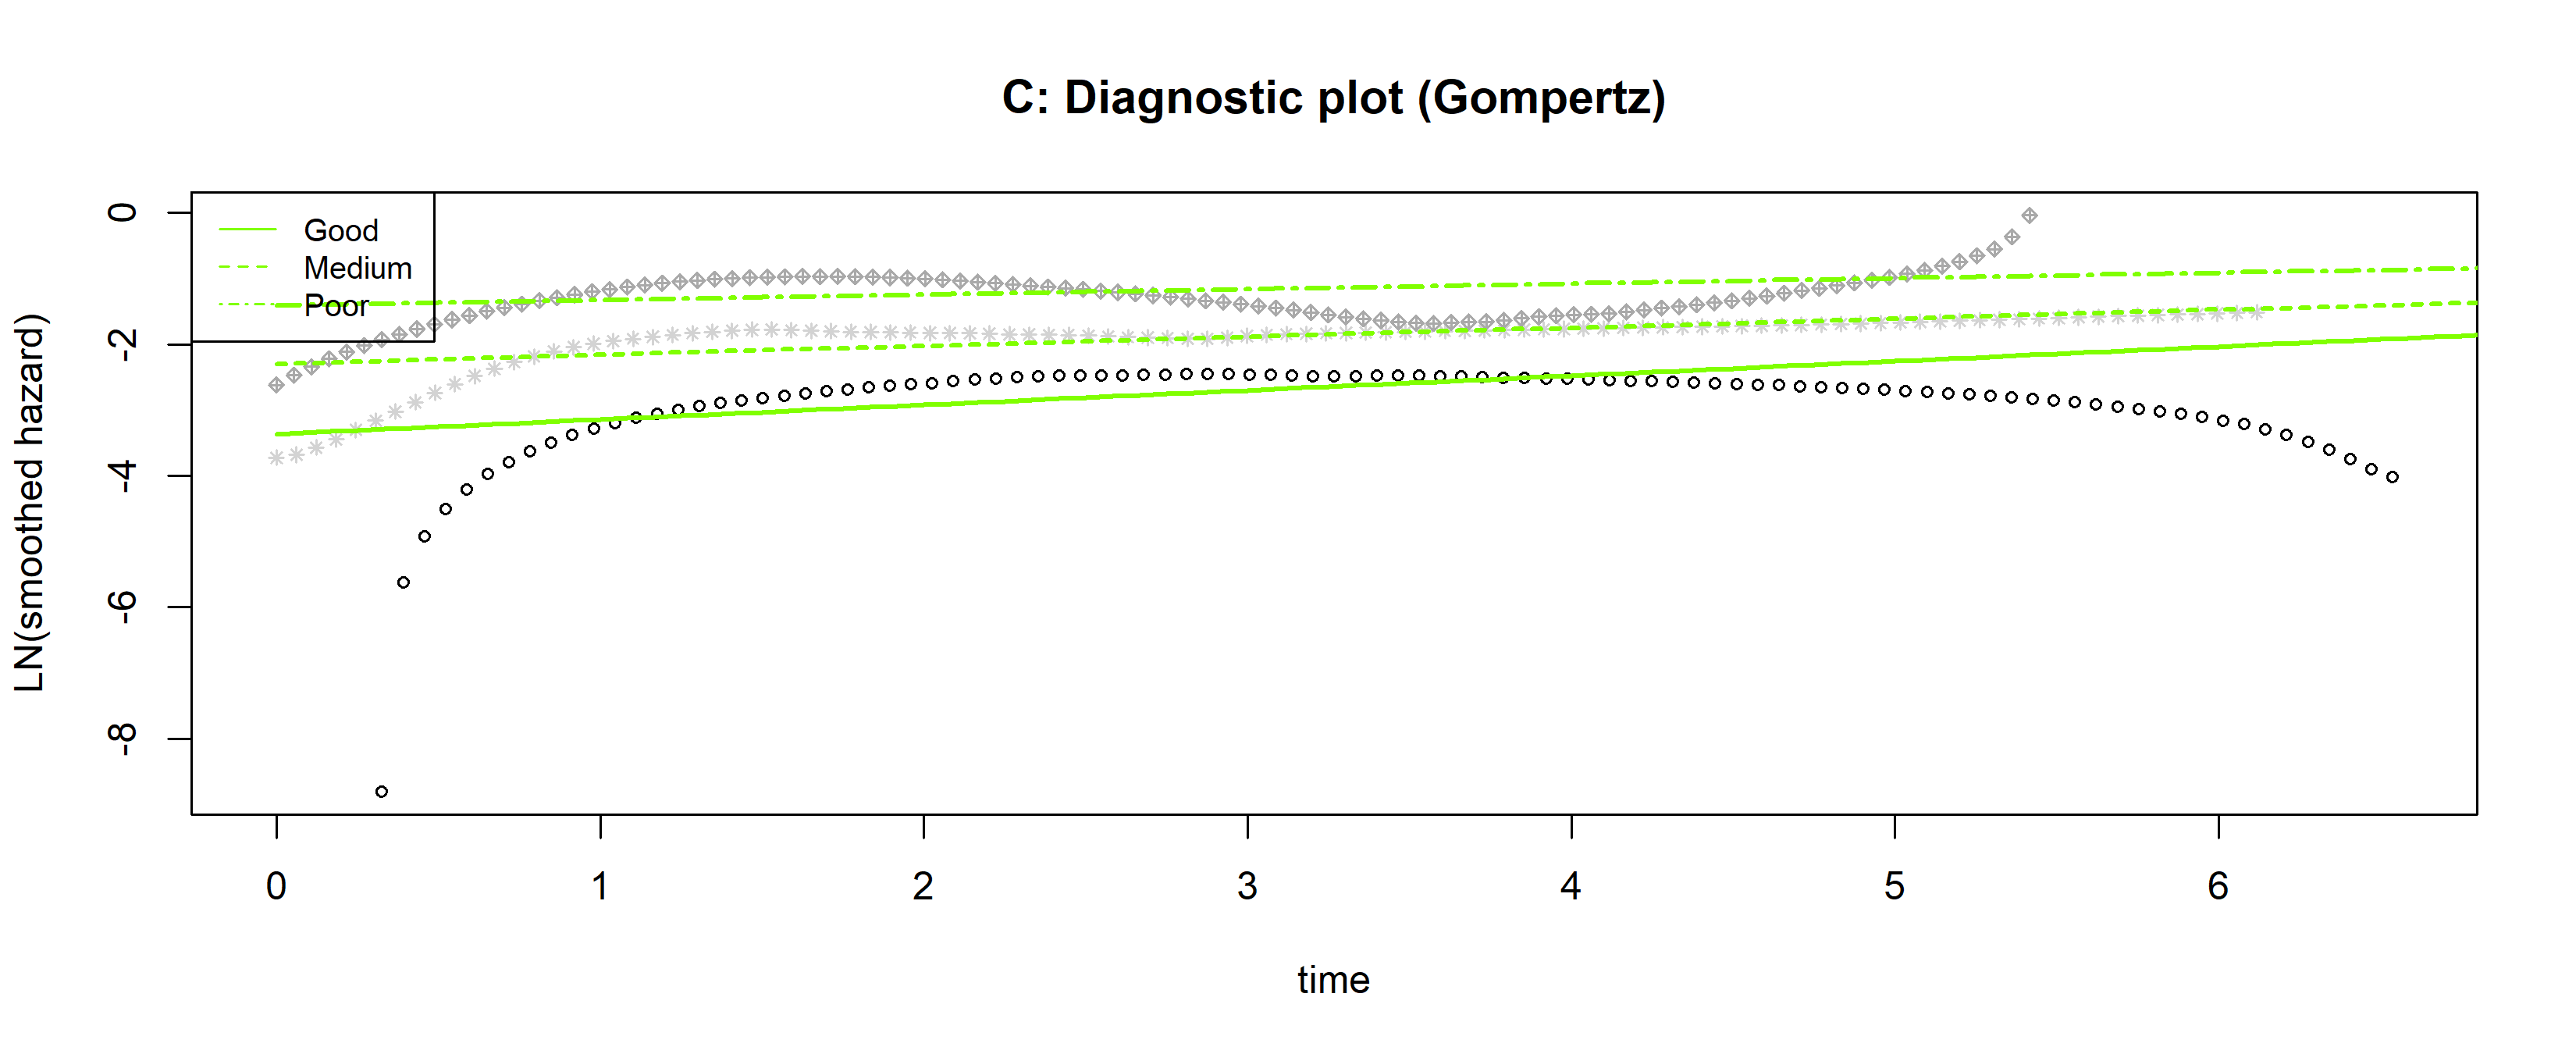
\includegraphics[height=0.3\textheight]{images/gom-3} \end{flushleft}

\subsection{Log-normal}\label{log-normal}

\begin{flushleft}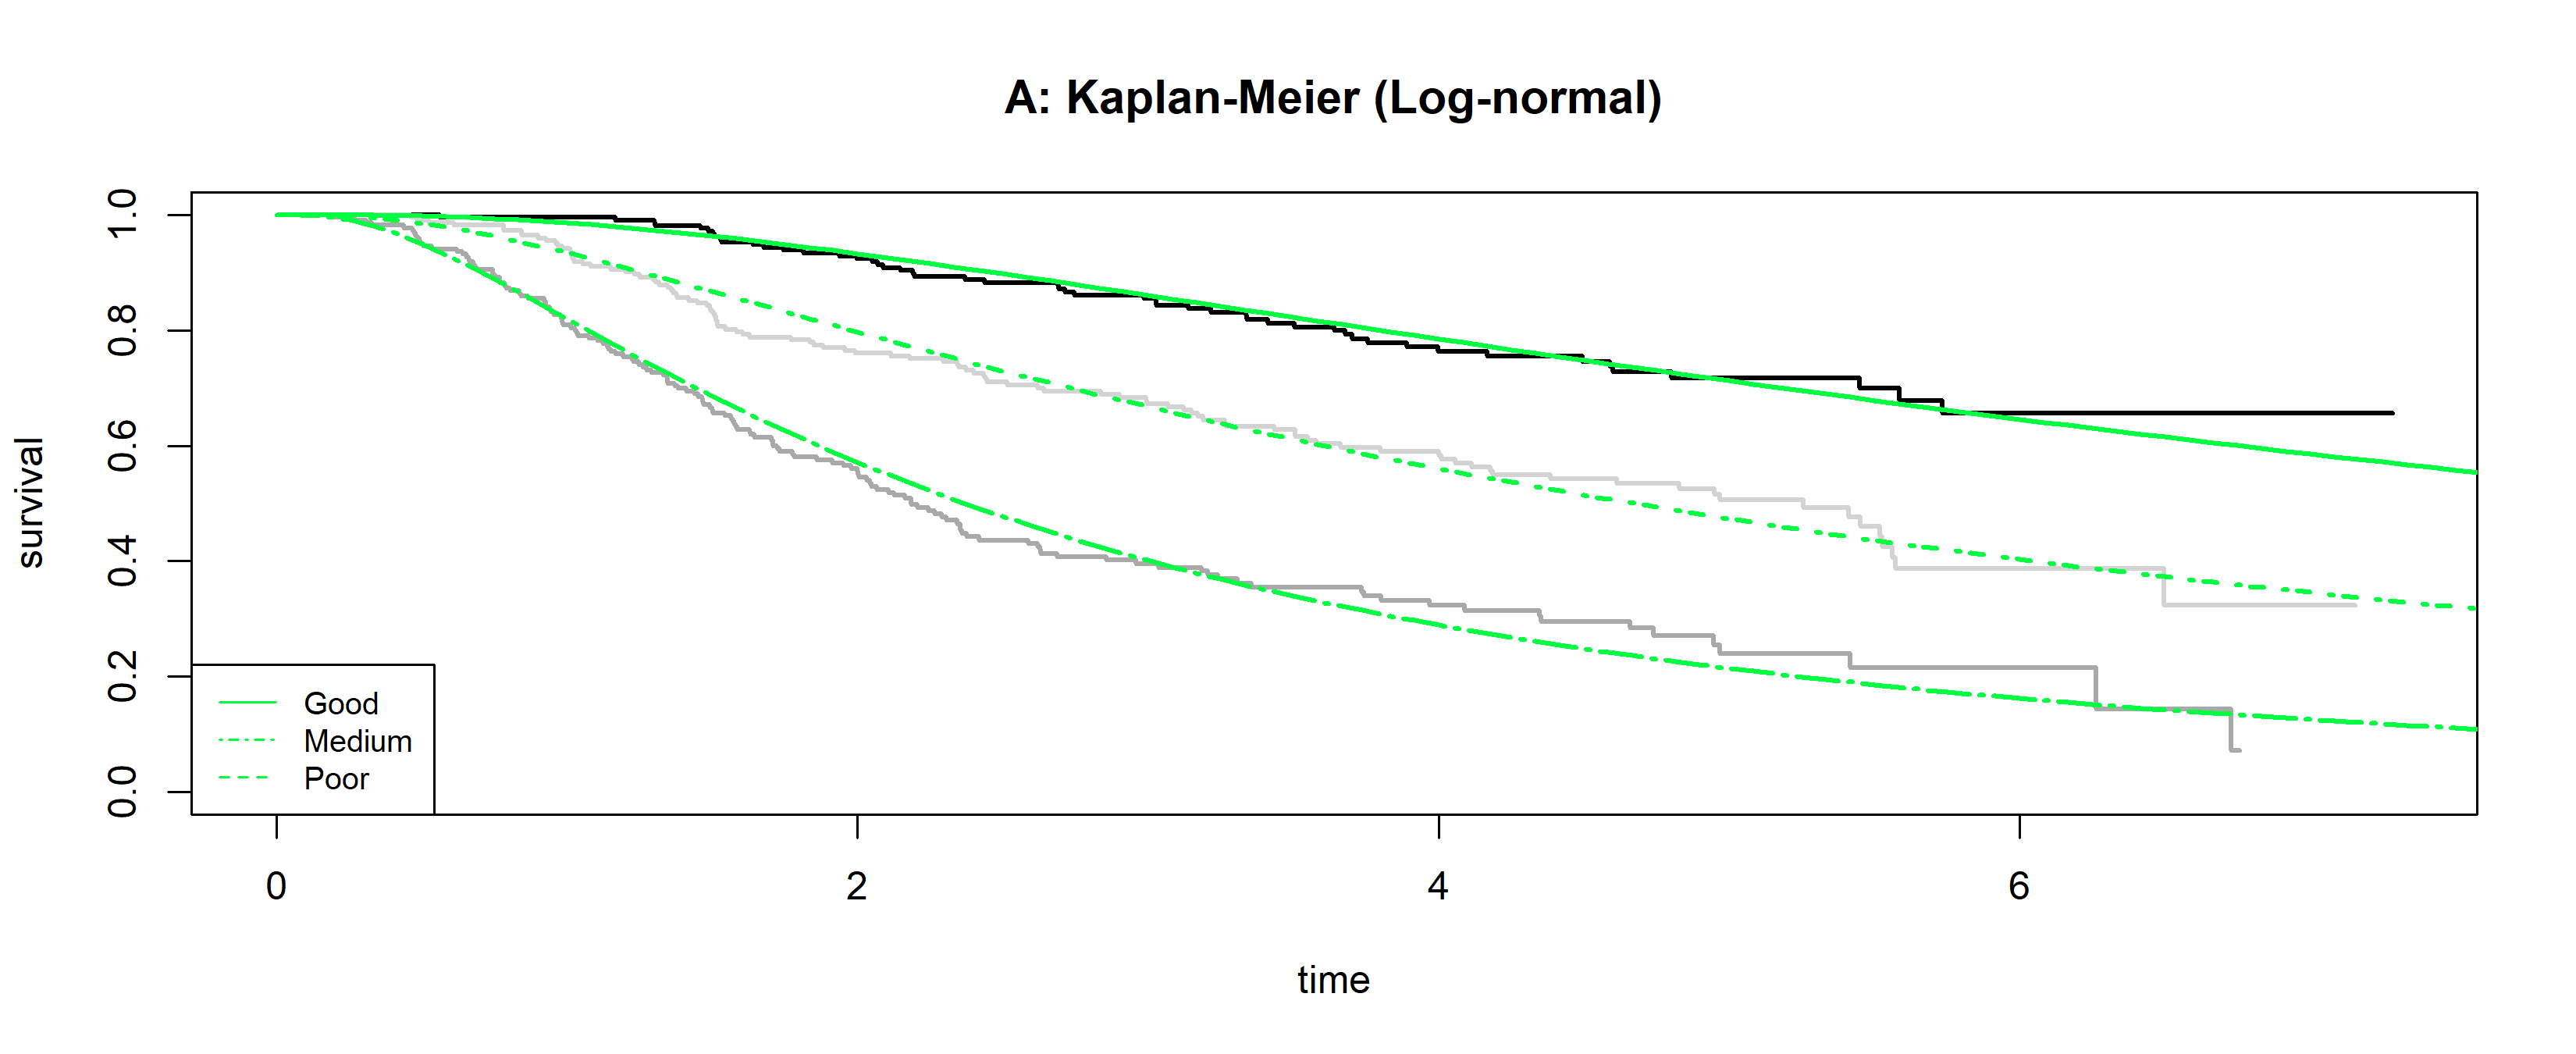
\includegraphics[height=0.3\textheight]{images/lnorm-1} \end{flushleft}

\begin{flushleft}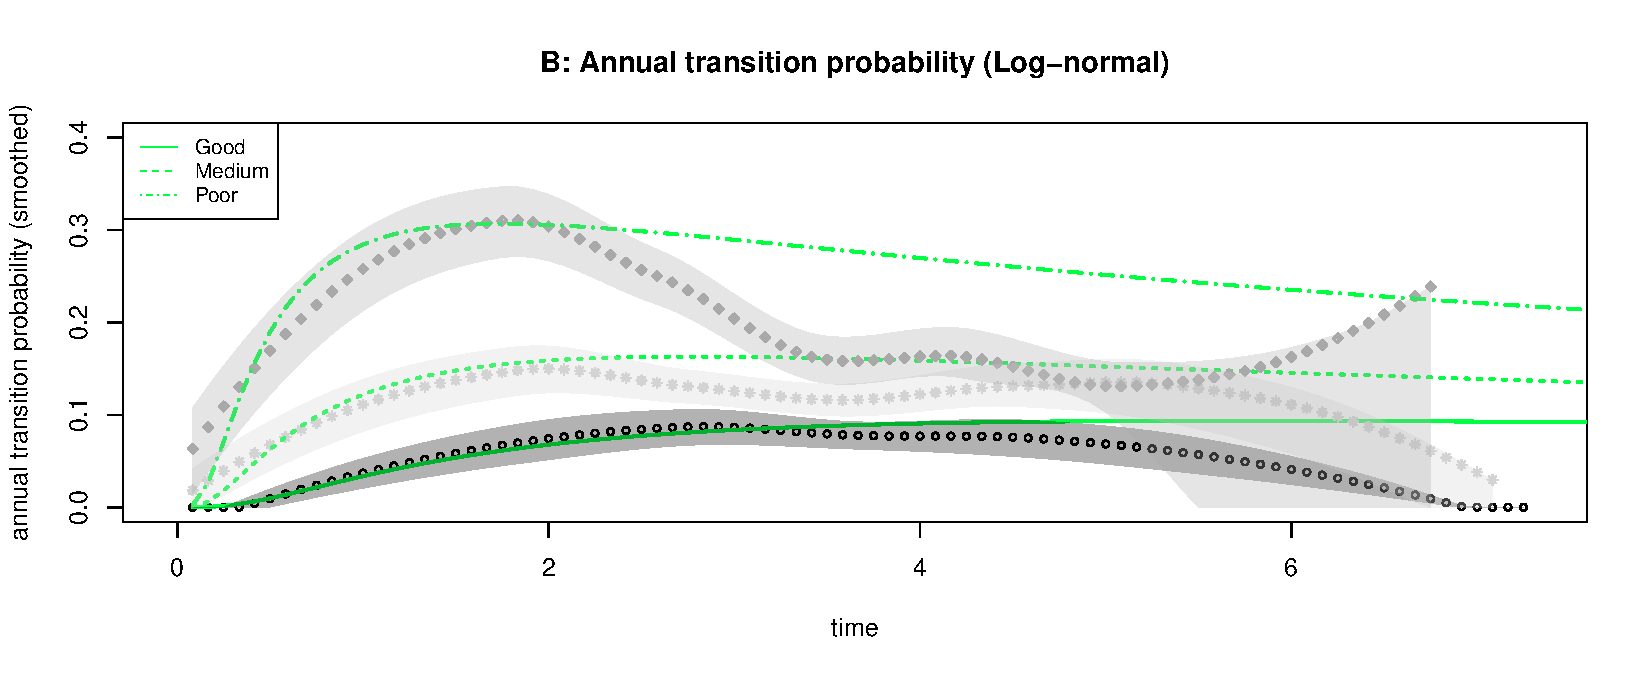
\includegraphics[height=0.3\textheight]{images/lnorm-2} \end{flushleft}

\begin{flushleft}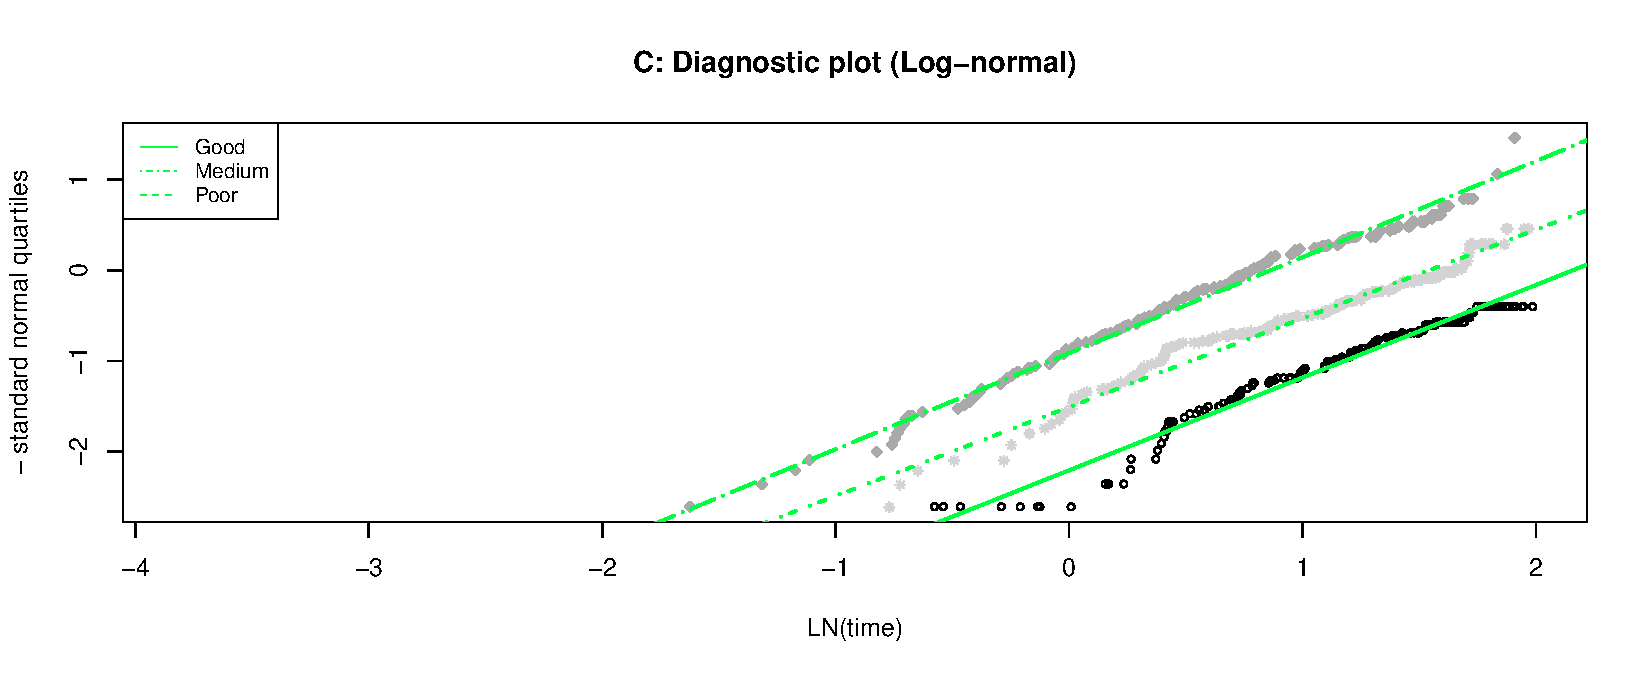
\includegraphics[height=0.3\textheight]{images/lnorm-3} \end{flushleft}

\subsection{Log-logistic}\label{log-logistic}

\begin{flushleft}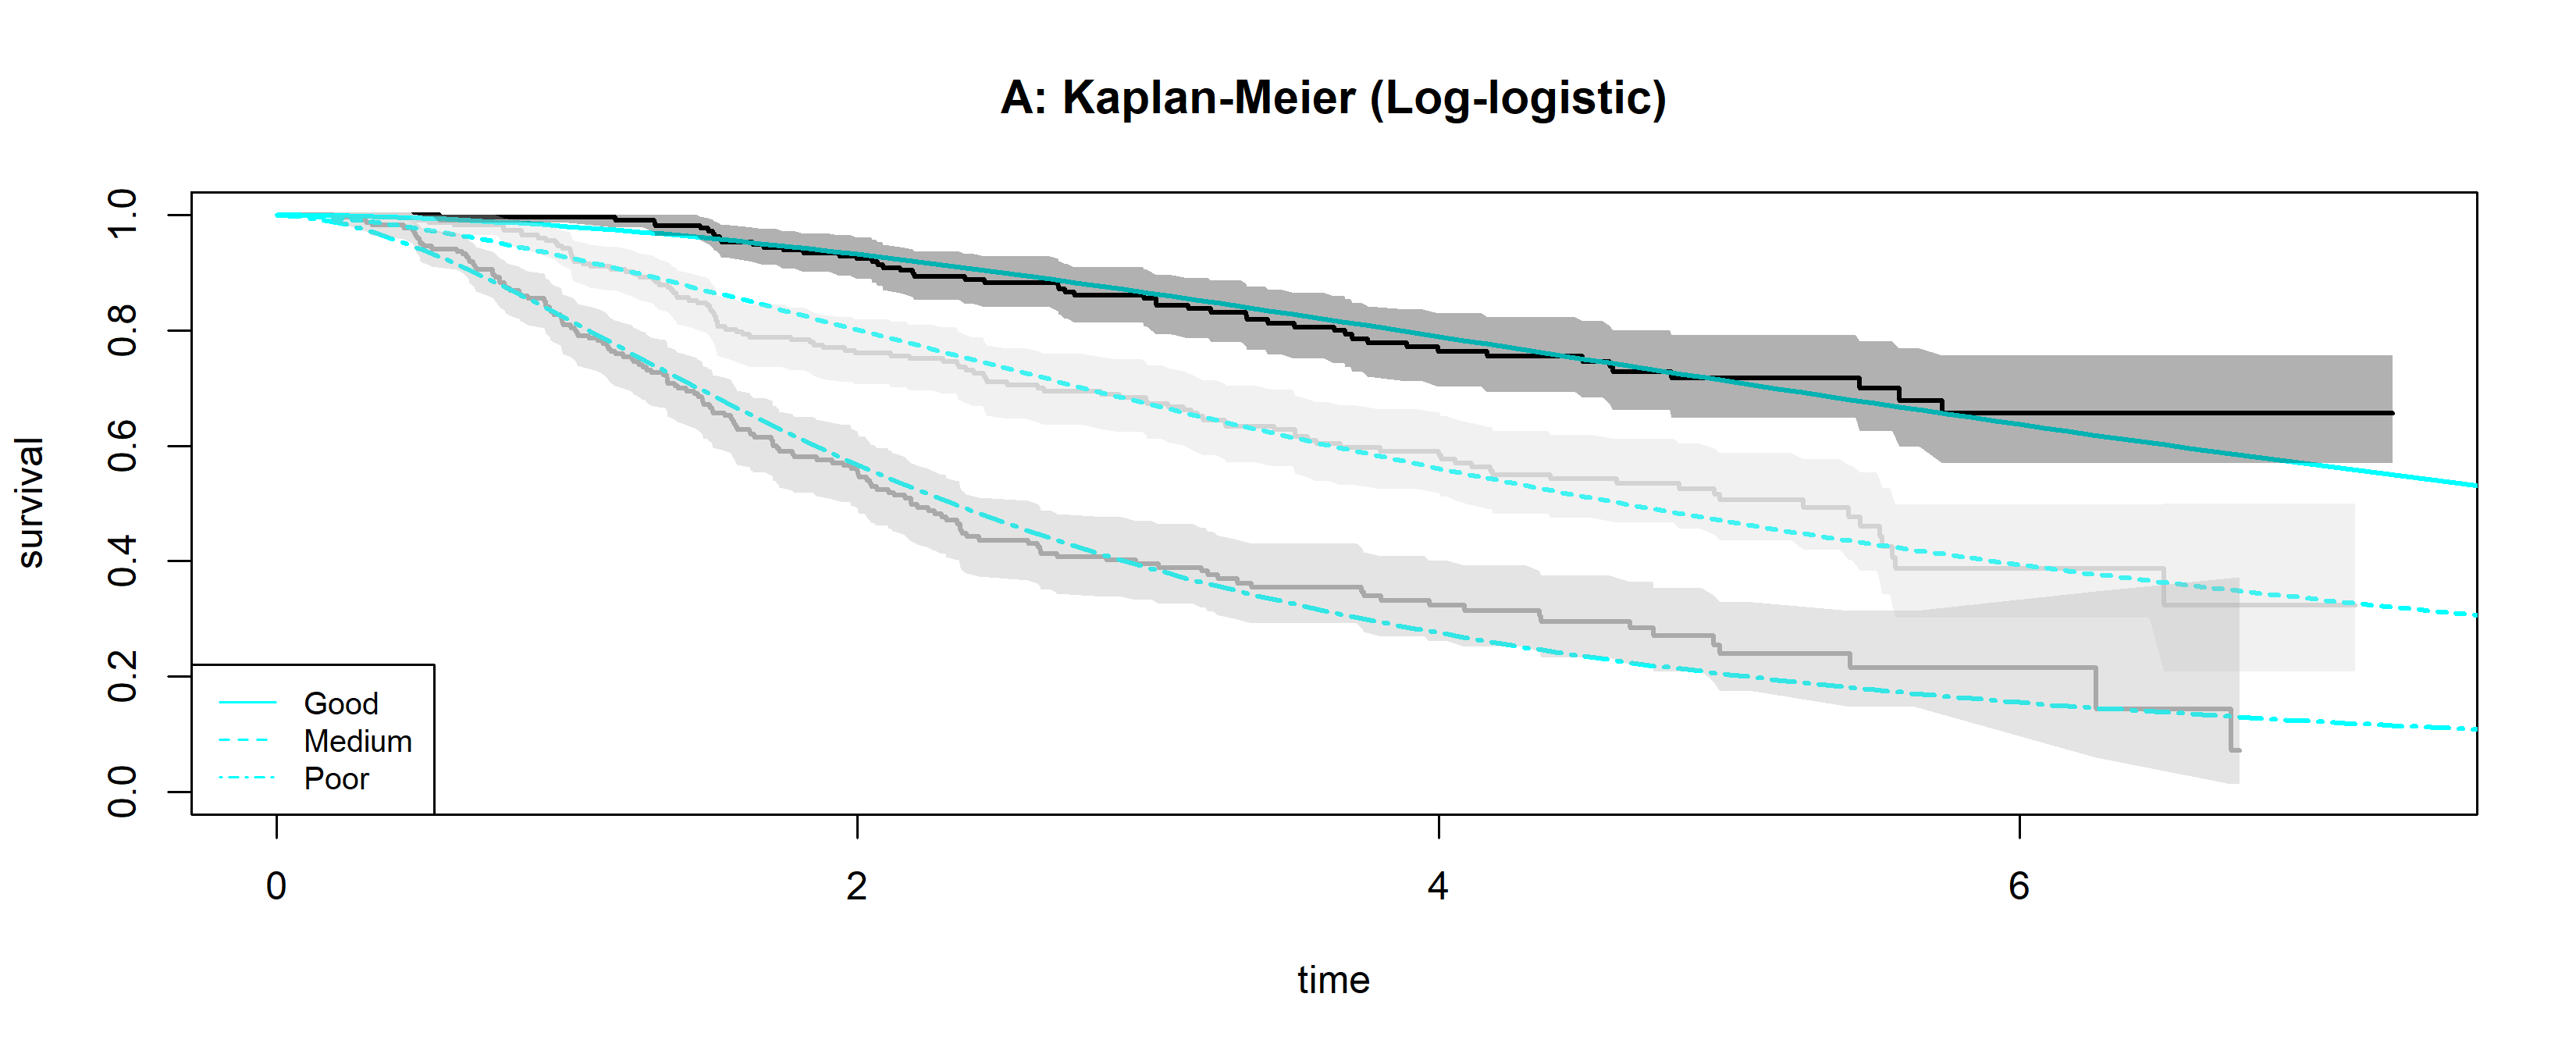
\includegraphics[height=0.3\textheight]{images/llog-1} \end{flushleft}

\begin{flushleft}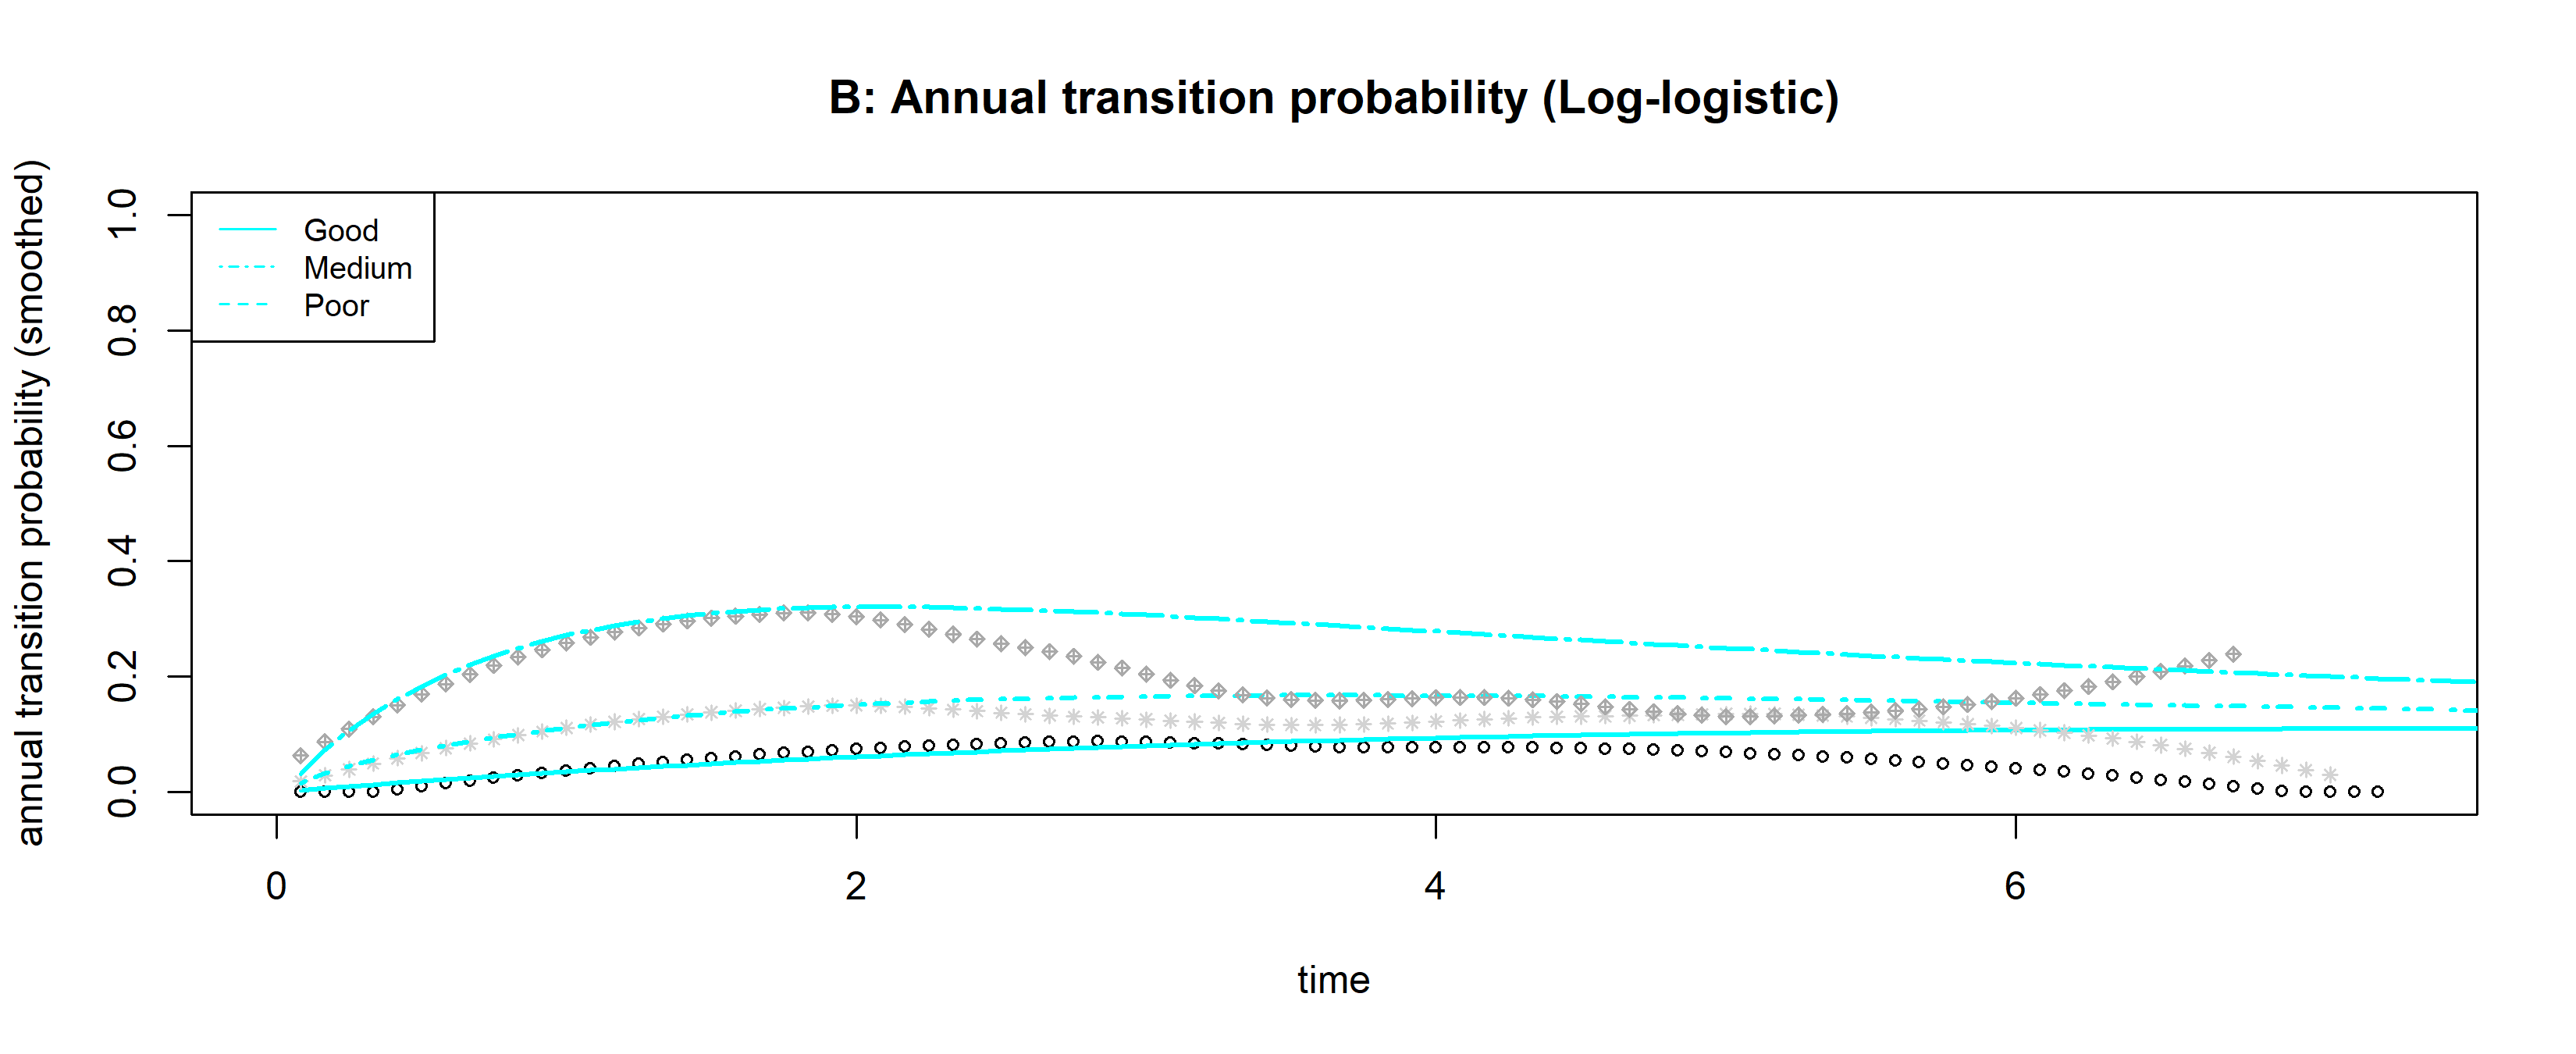
\includegraphics[height=0.3\textheight]{images/llog-2} \end{flushleft}

\begin{flushleft}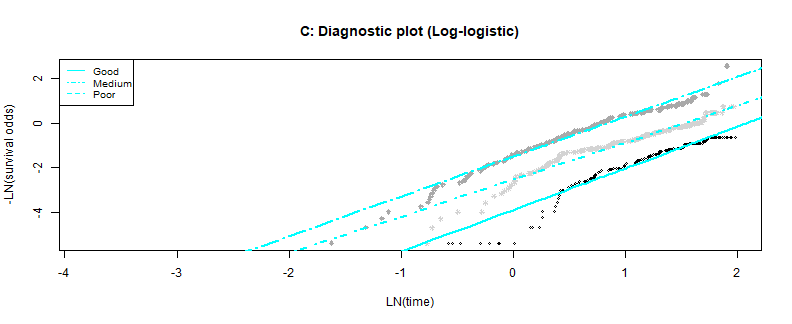
\includegraphics[height=0.3\textheight]{images/llog-3} \end{flushleft}

\subsection{Gamma}\label{gamma}

\begin{flushleft}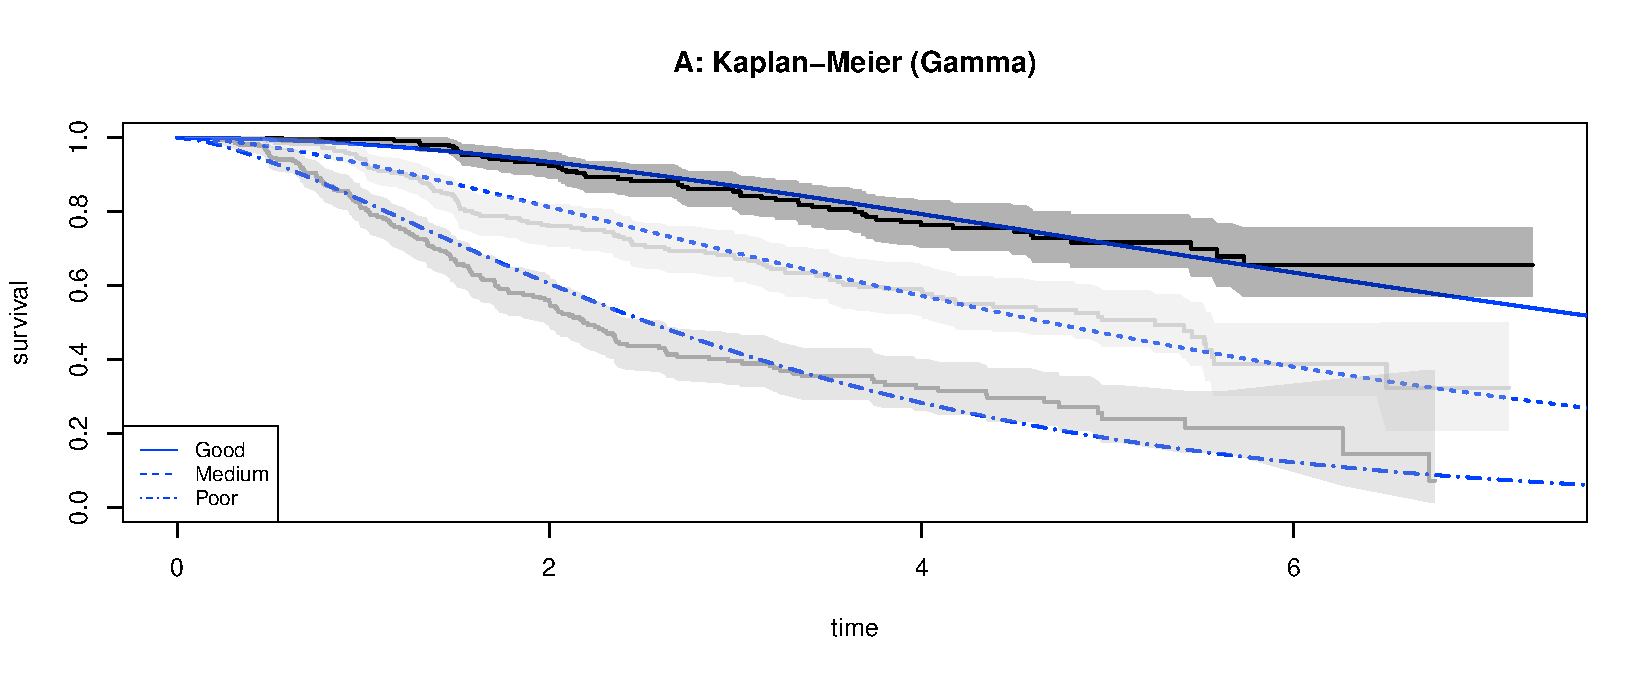
\includegraphics[height=0.3\textheight]{images/gam-1} \end{flushleft}

\begin{flushleft}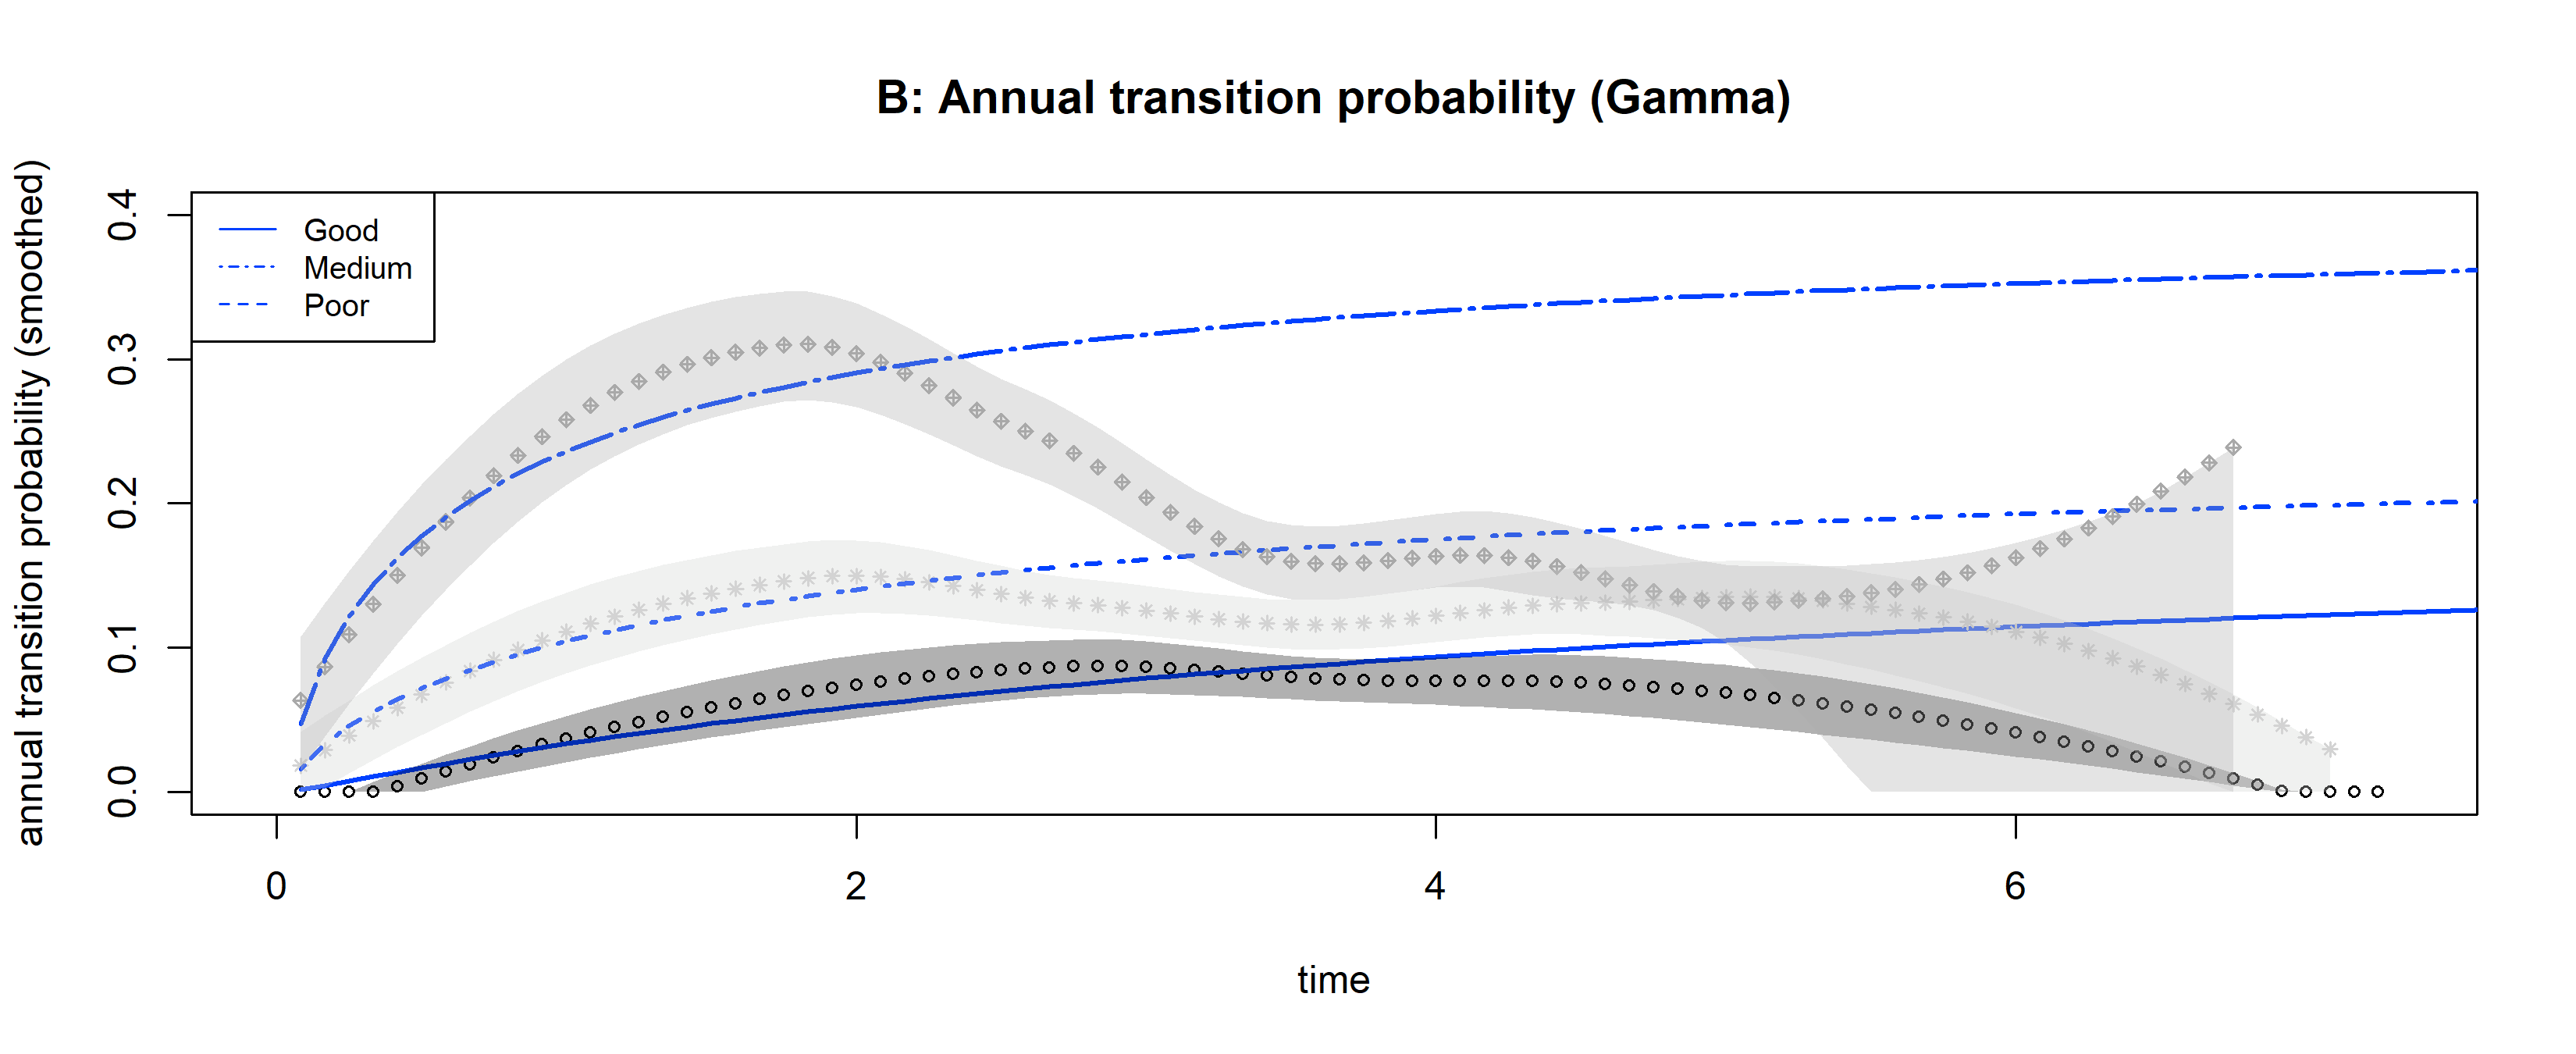
\includegraphics[height=0.3\textheight]{images/gam-2} \end{flushleft}

\begin{flushleft}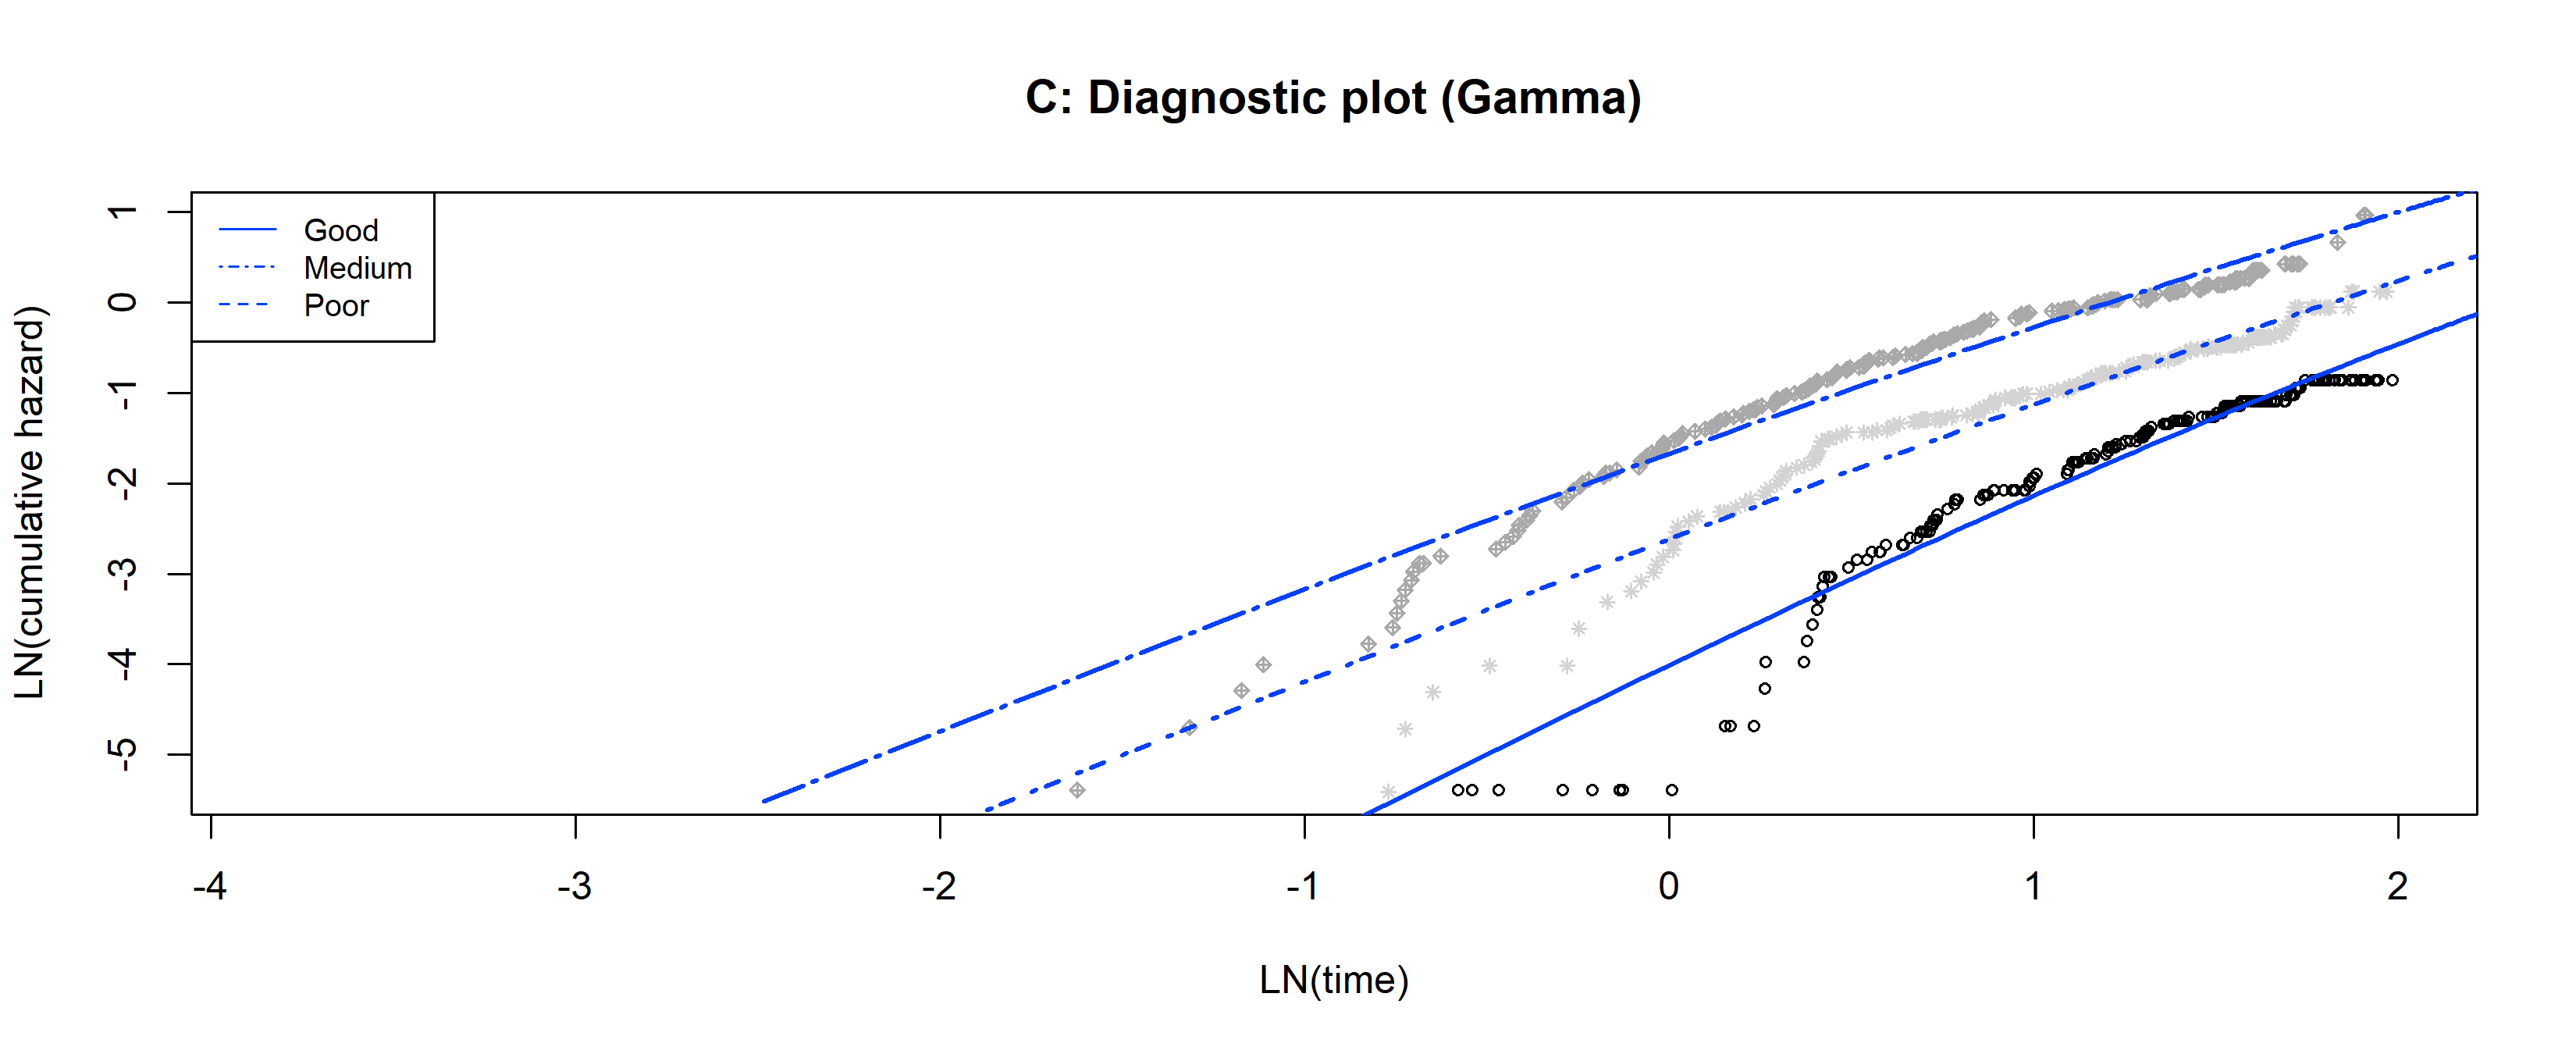
\includegraphics[height=0.3\textheight]{images/gam-3} \end{flushleft}

\subsection{Generalised Gamma}\label{generalised-gamma}

\begin{flushleft}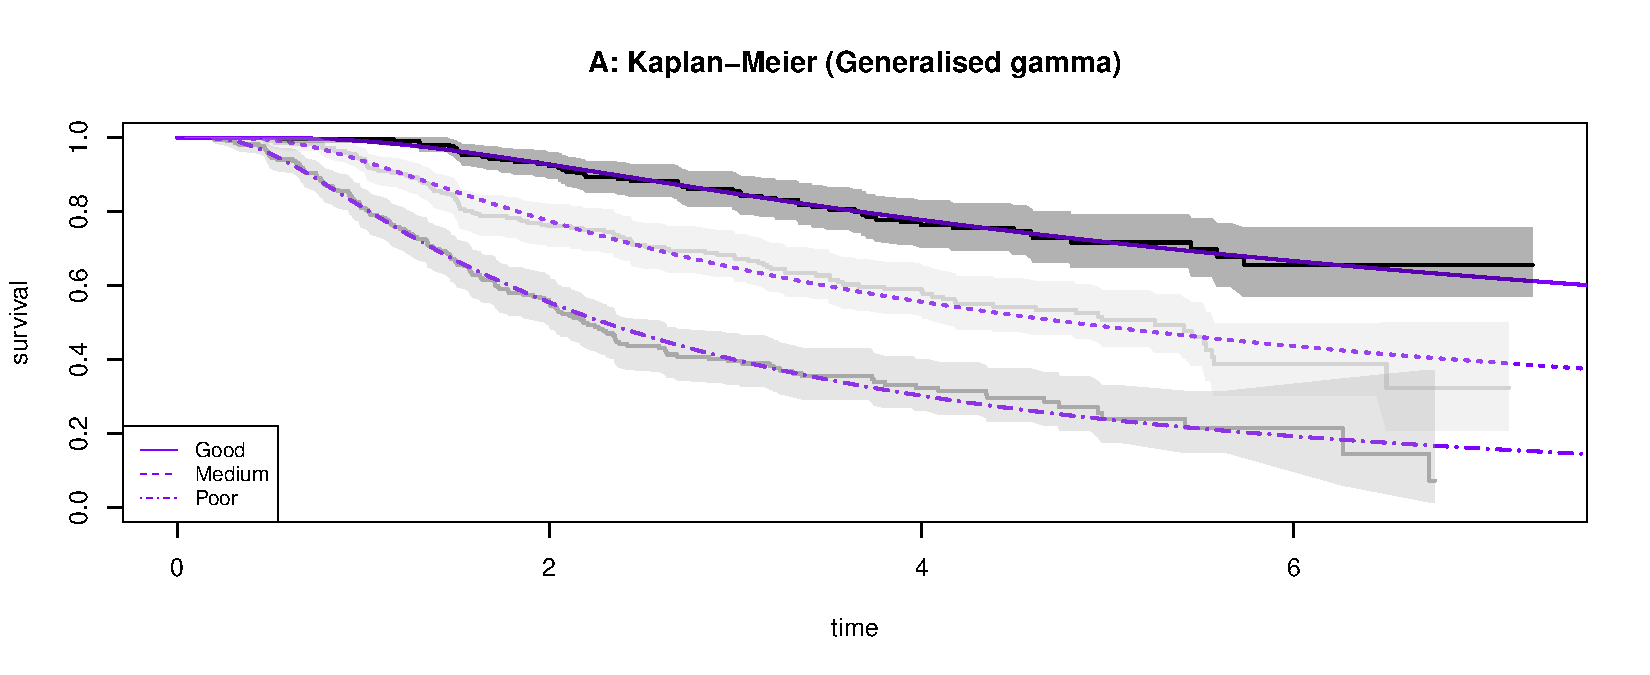
\includegraphics[height=0.3\textheight]{images/ggam-1} \end{flushleft}

\begin{flushleft}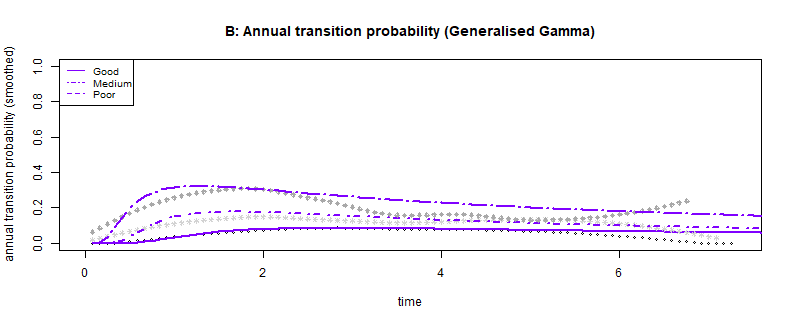
\includegraphics[height=0.3\textheight]{images/ggam-2} \end{flushleft}

\begin{flushleft}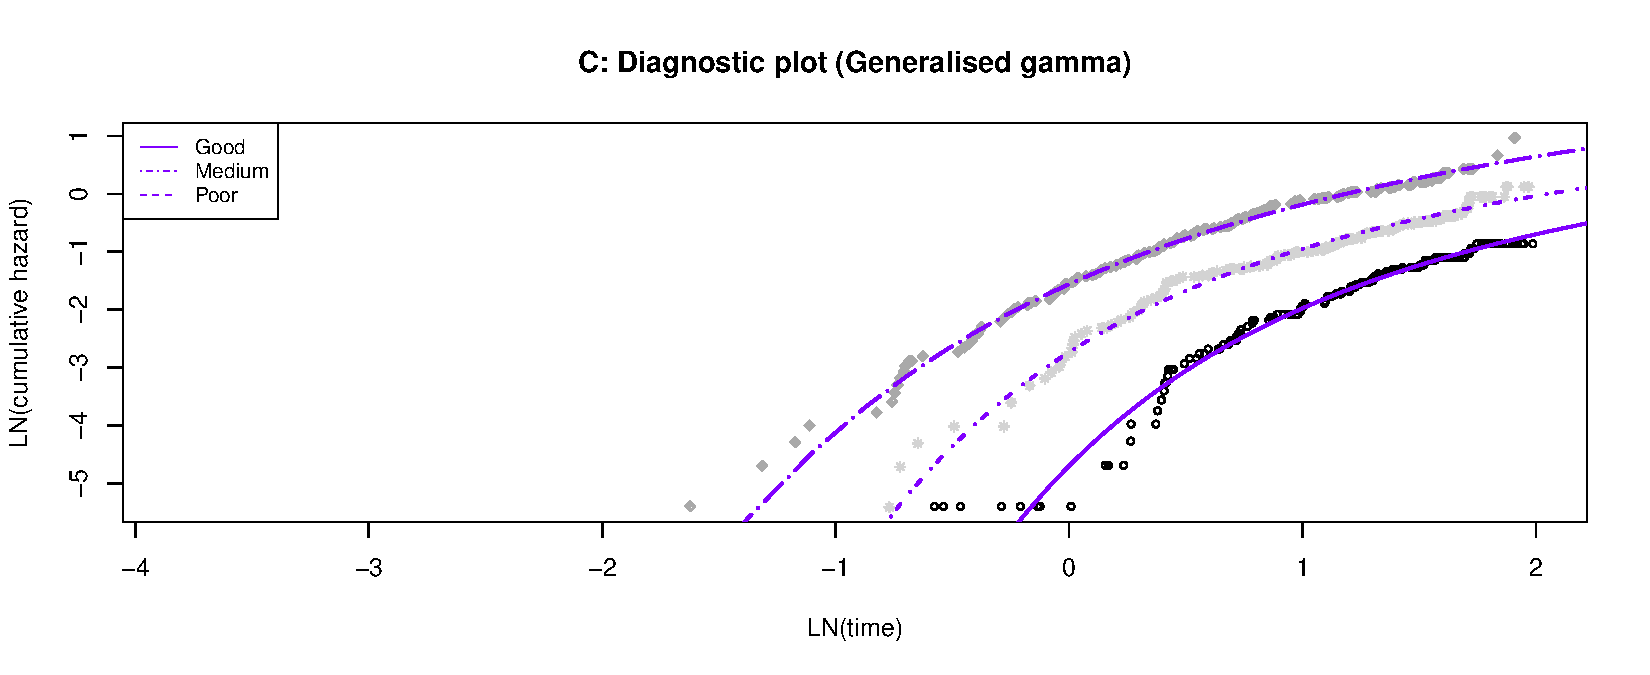
\includegraphics[height=0.3\textheight]{images/ggam-3} \end{flushleft}

\newpage

\section{Parametric spline models?}\label{parametric-spline-models}

If standard parametric models are not appropriate, are spline models a
more appropriate fit to the data?

\begin{flushleft}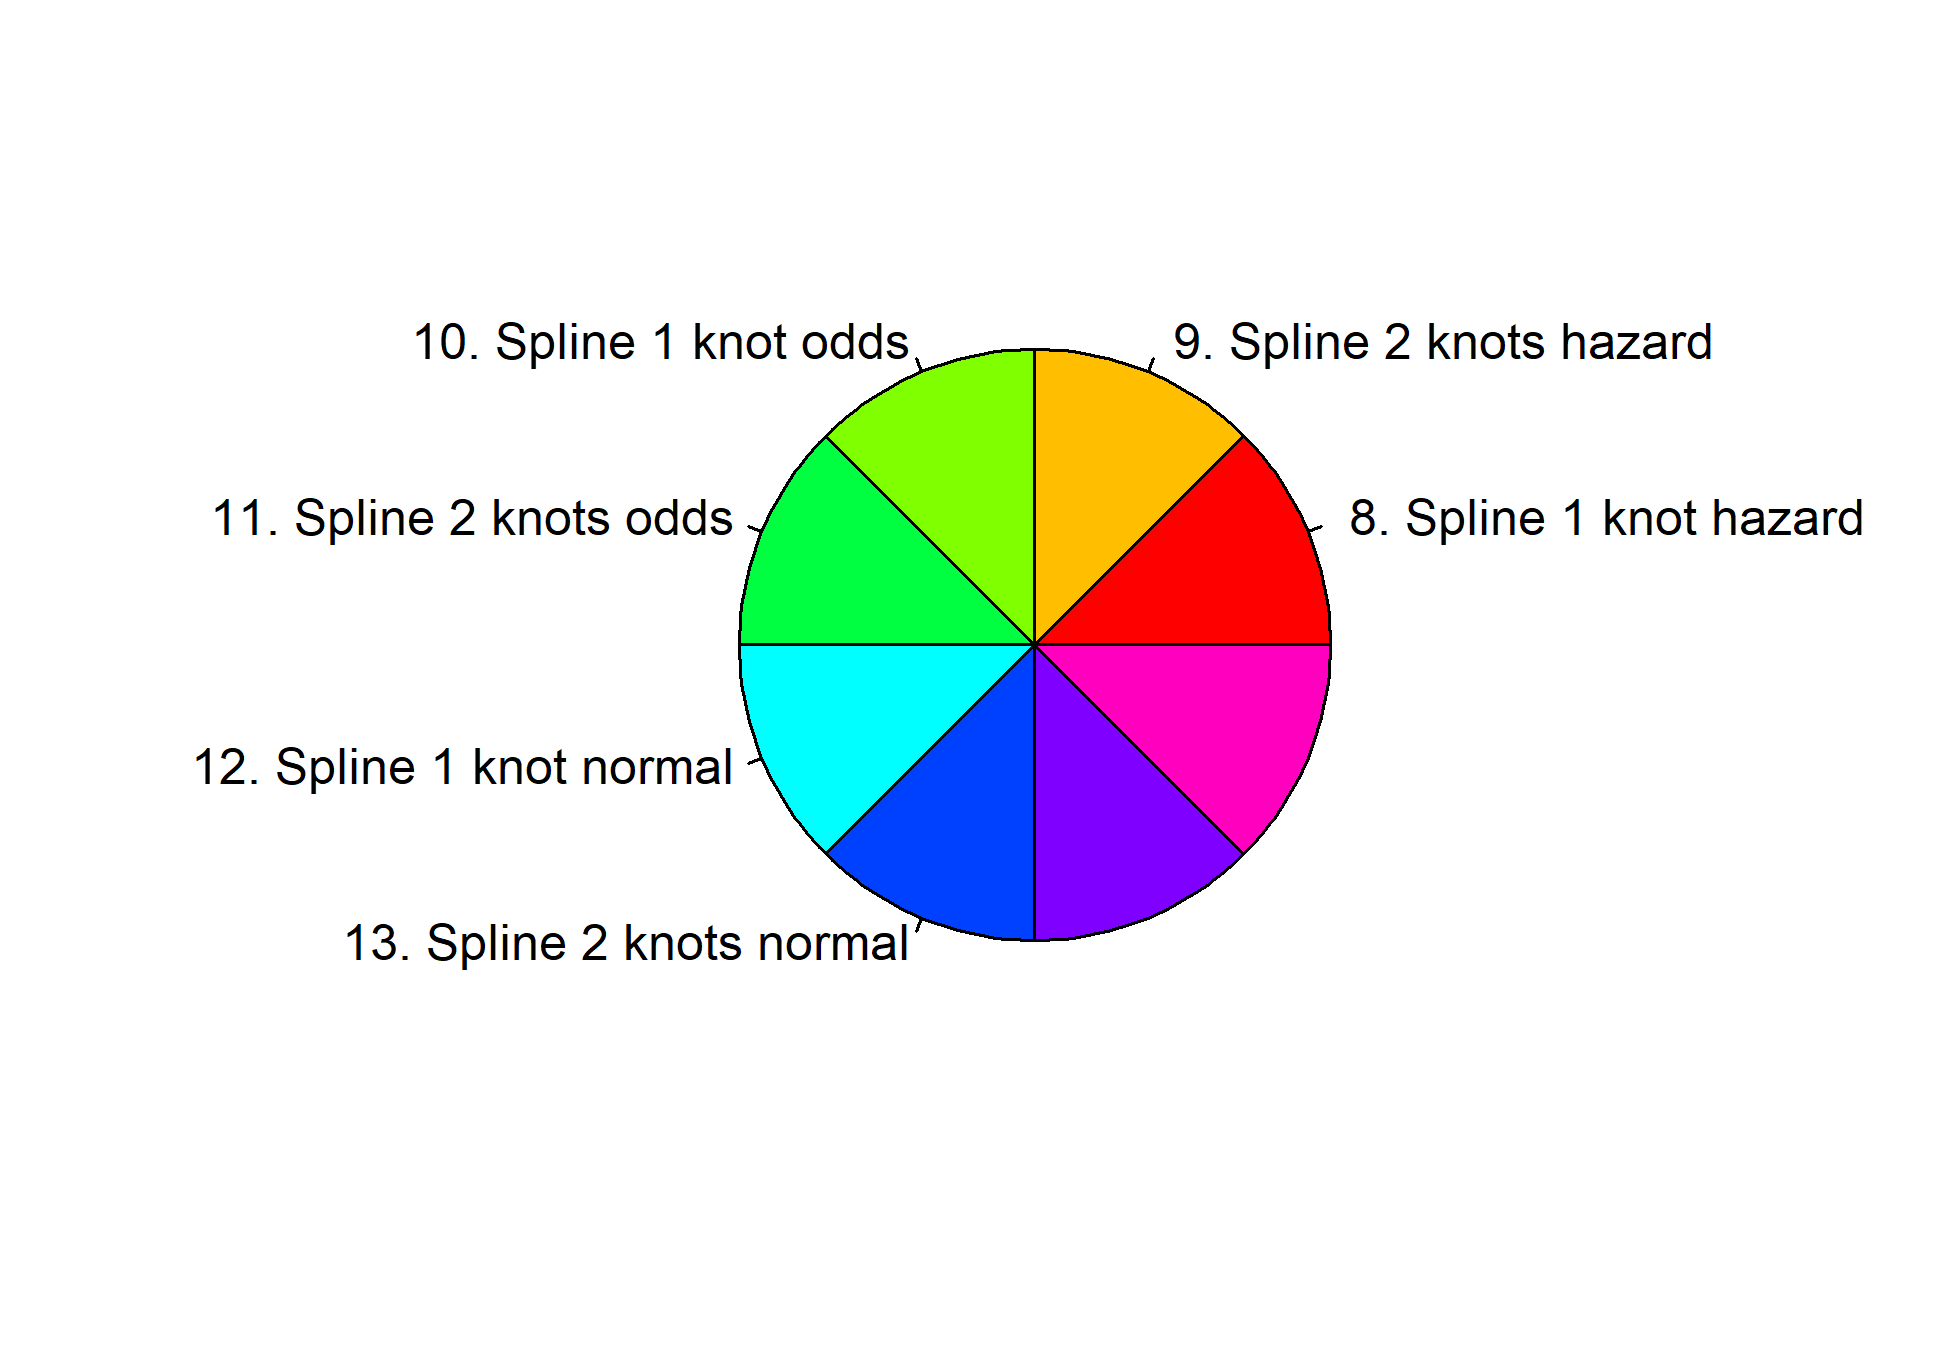
\includegraphics{images/spline-1} \end{flushleft}

\begin{table}[H]
\centering
\begin{tabular}{lrr}
\toprule
Model & AIC & BIC\\
\midrule
\rowcolor{gray!6}  9. Spline 2 knots hazard & 1585.894 & 1640.264\\
11. Spline 2 knots odds & 1587.289 & 1641.659\\
\rowcolor{gray!6}  12. Spline 1 knot normal & 1587.682 & 1628.460\\
13. Spline 2 knots normal & 1588.343 & 1642.714\\
\rowcolor{gray!6}  7. Generalised Gamma & 1589.049 & 1629.826\\
8. Spline 1 knot hazard & 1589.327 & 1630.105\\
\rowcolor{gray!6}  10. Spline 1 knot odds & 1590.221 & 1630.999\\
4. Log-normal & 1592.880 & 1620.066\\
\rowcolor{gray!6}  5. Log-logistic & 1609.294 & 1636.479\\
6. Gamma & 1621.982 & 1649.167\\
\rowcolor{gray!6}  2. Weibull & 1632.618 & 1659.803\\
3. Gompertz & 1660.954 & 1688.140\\
\rowcolor{gray!6}  1. Exponential & 1668.212 & 1681.805\\
\bottomrule
\end{tabular}
\end{table}

\subsection{Spline hazard 1 knot}\label{spline-hazard-1-knot}

\begin{flushleft}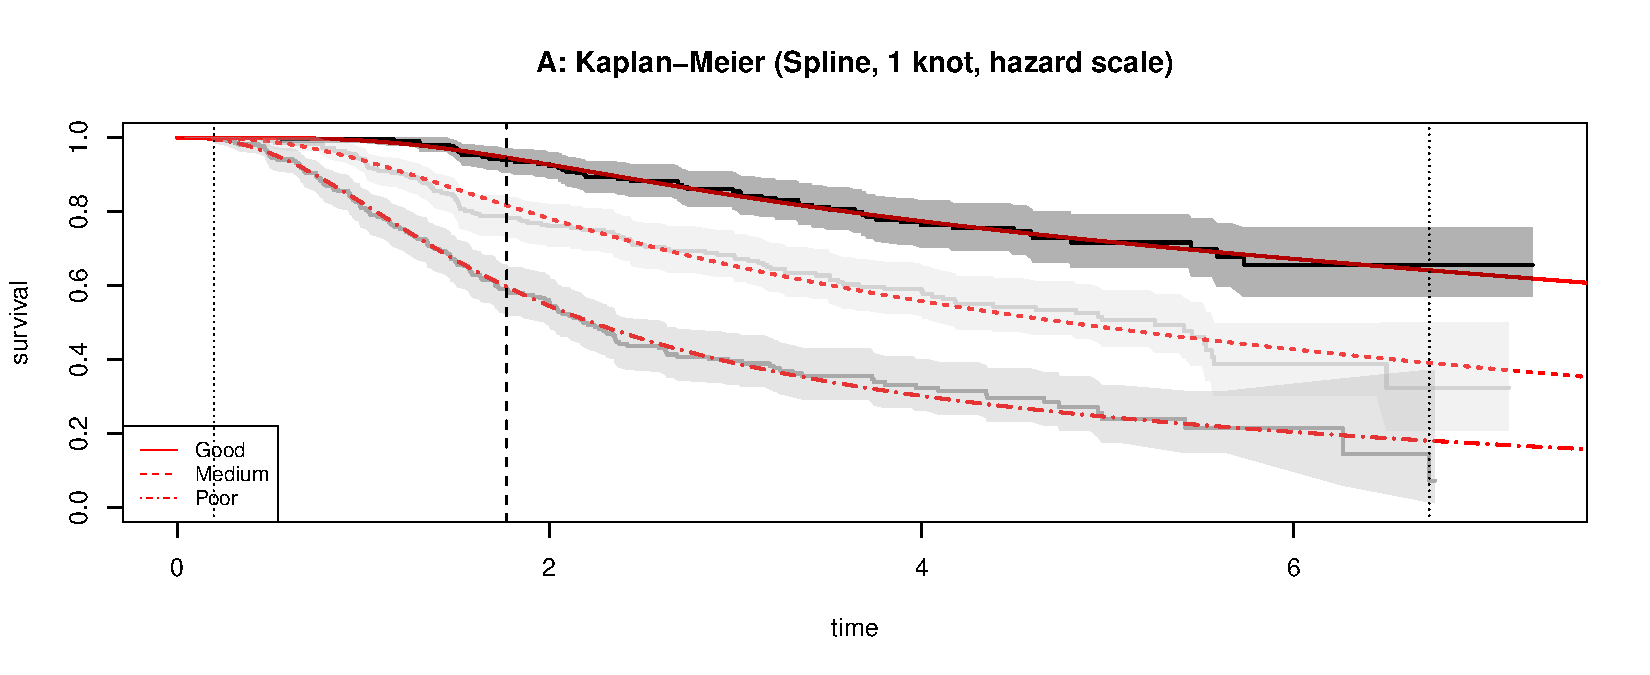
\includegraphics[height=0.3\textheight]{images/spline_hazard1-1} \end{flushleft}

\begin{flushleft}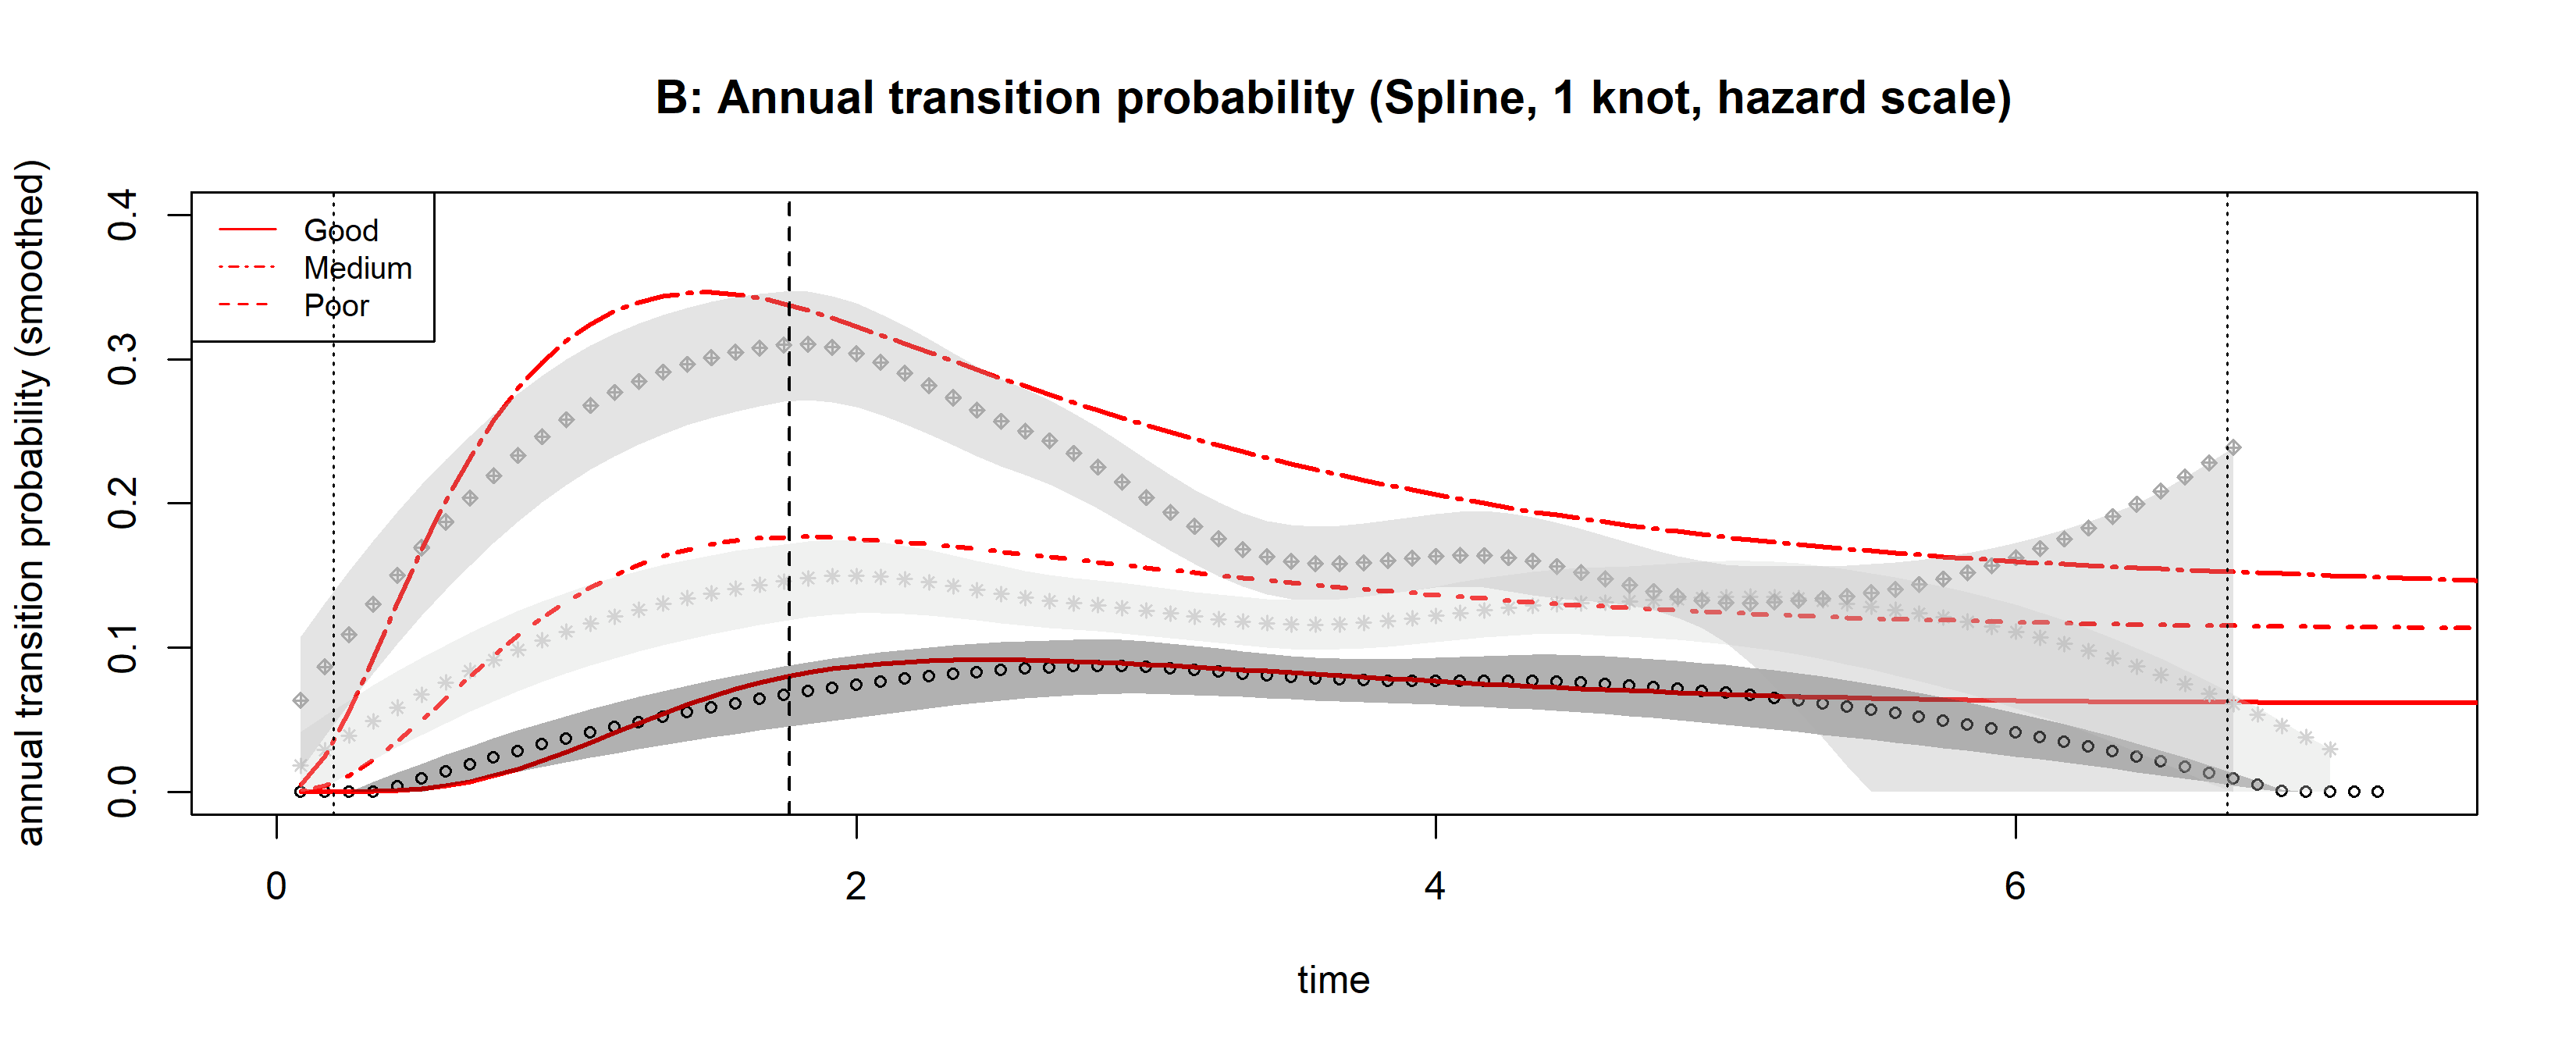
\includegraphics[height=0.3\textheight]{images/spline_hazard1-2} \end{flushleft}

\begin{flushleft}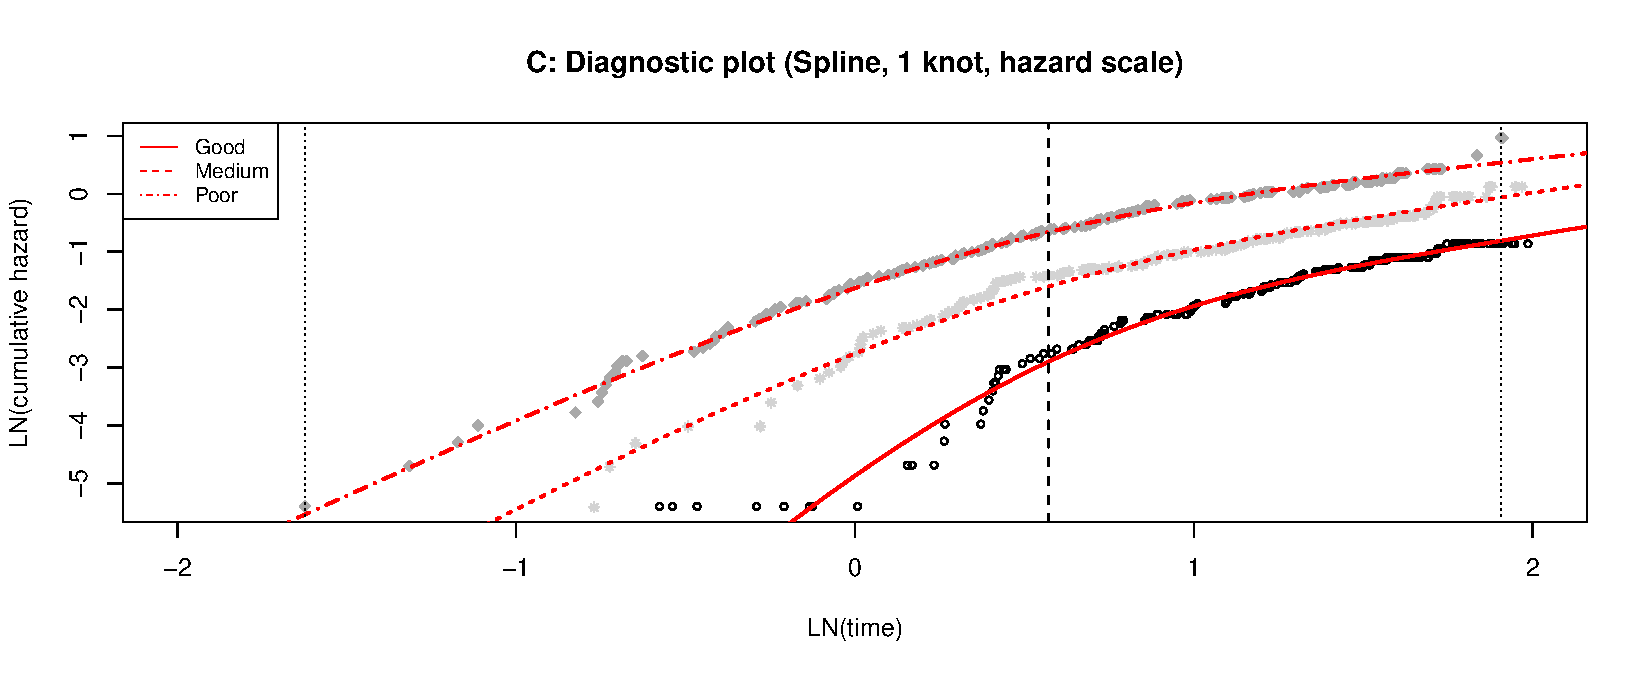
\includegraphics[height=0.3\textheight]{images/spline_hazard1-3} \end{flushleft}

\subsection{Spline hazard 2 knots}\label{spline-hazard-2-knots}

\begin{flushleft}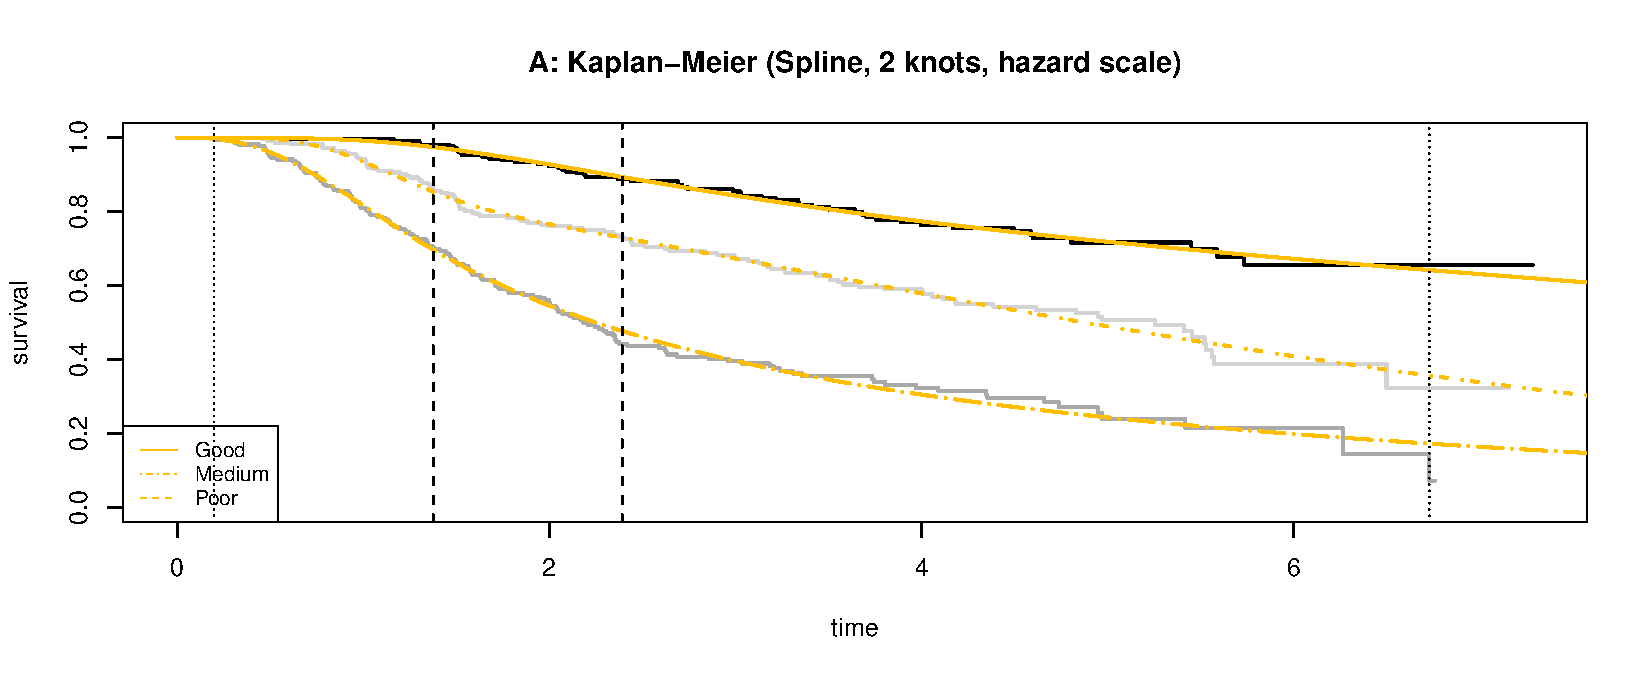
\includegraphics[height=0.3\textheight]{images/spline_hazard2-1} \end{flushleft}

\begin{flushleft}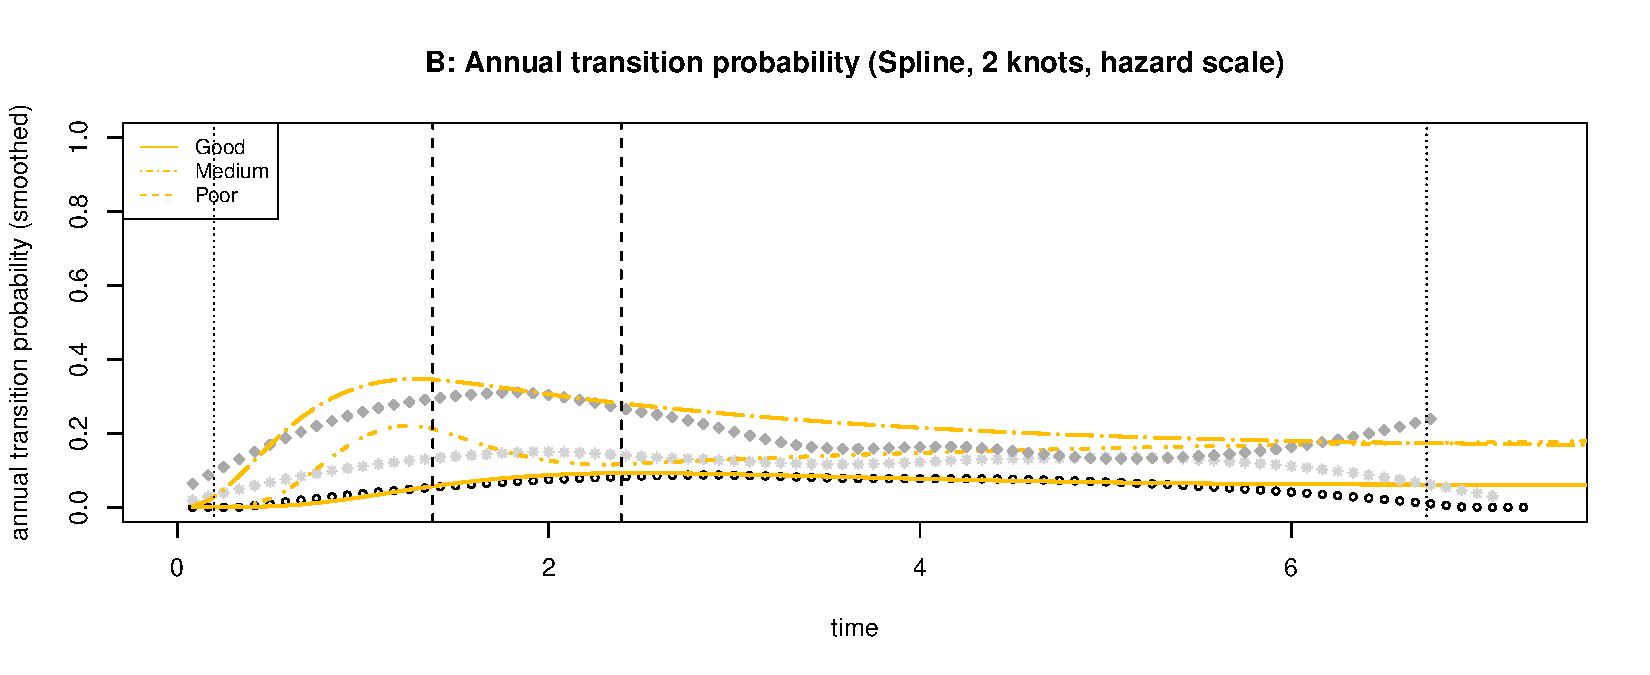
\includegraphics[height=0.3\textheight]{images/spline_hazard2-2} \end{flushleft}

\begin{flushleft}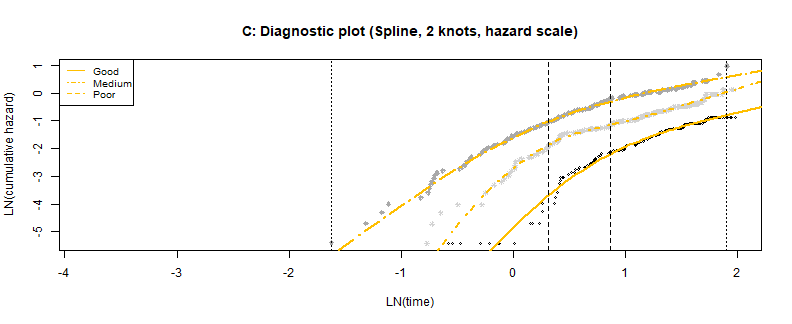
\includegraphics[height=0.3\textheight]{images/spline_hazard2-3} \end{flushleft}

\subsection{Spline odds 1 knot}\label{spline-odds-1-knot}

\begin{flushleft}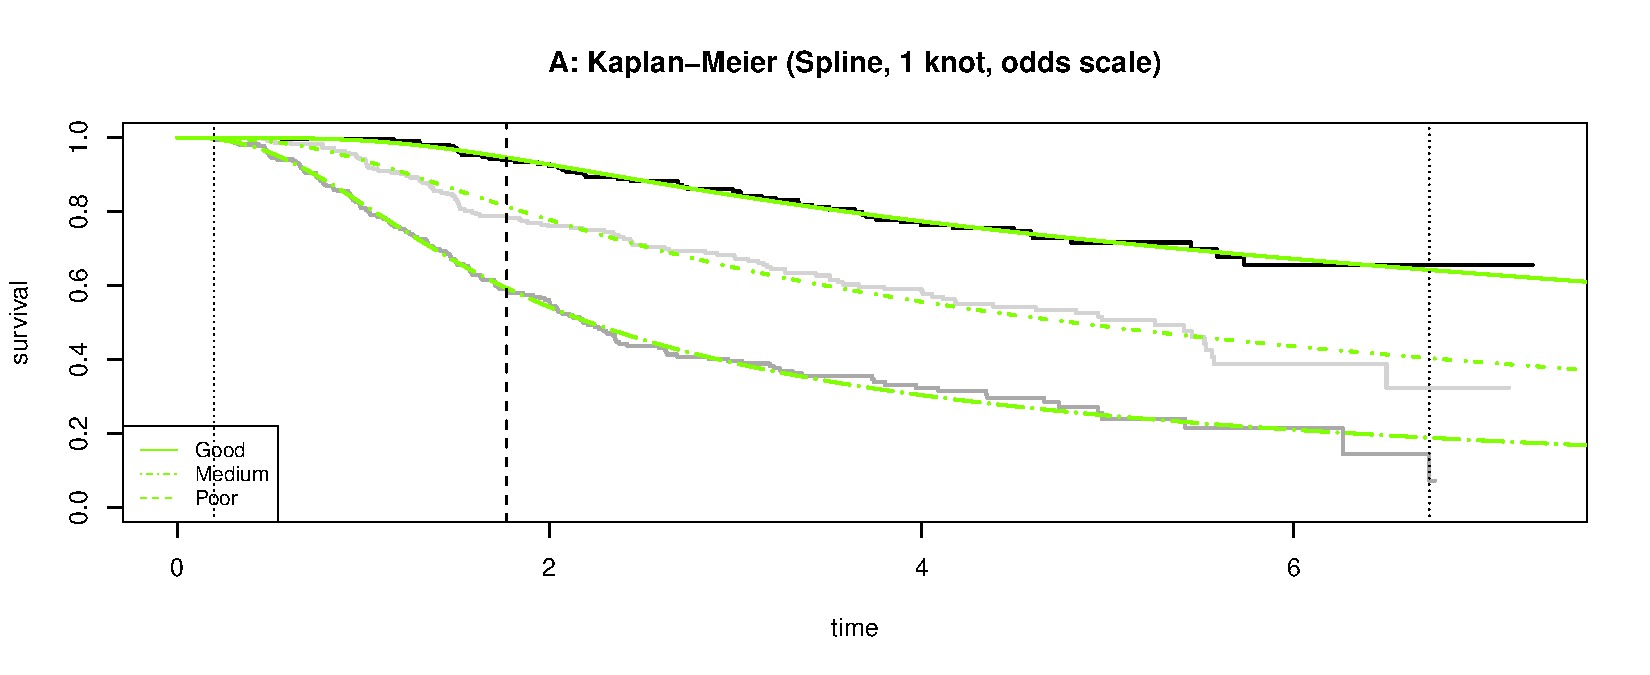
\includegraphics[height=0.3\textheight]{images/spline_odds1-1} \end{flushleft}

\begin{flushleft}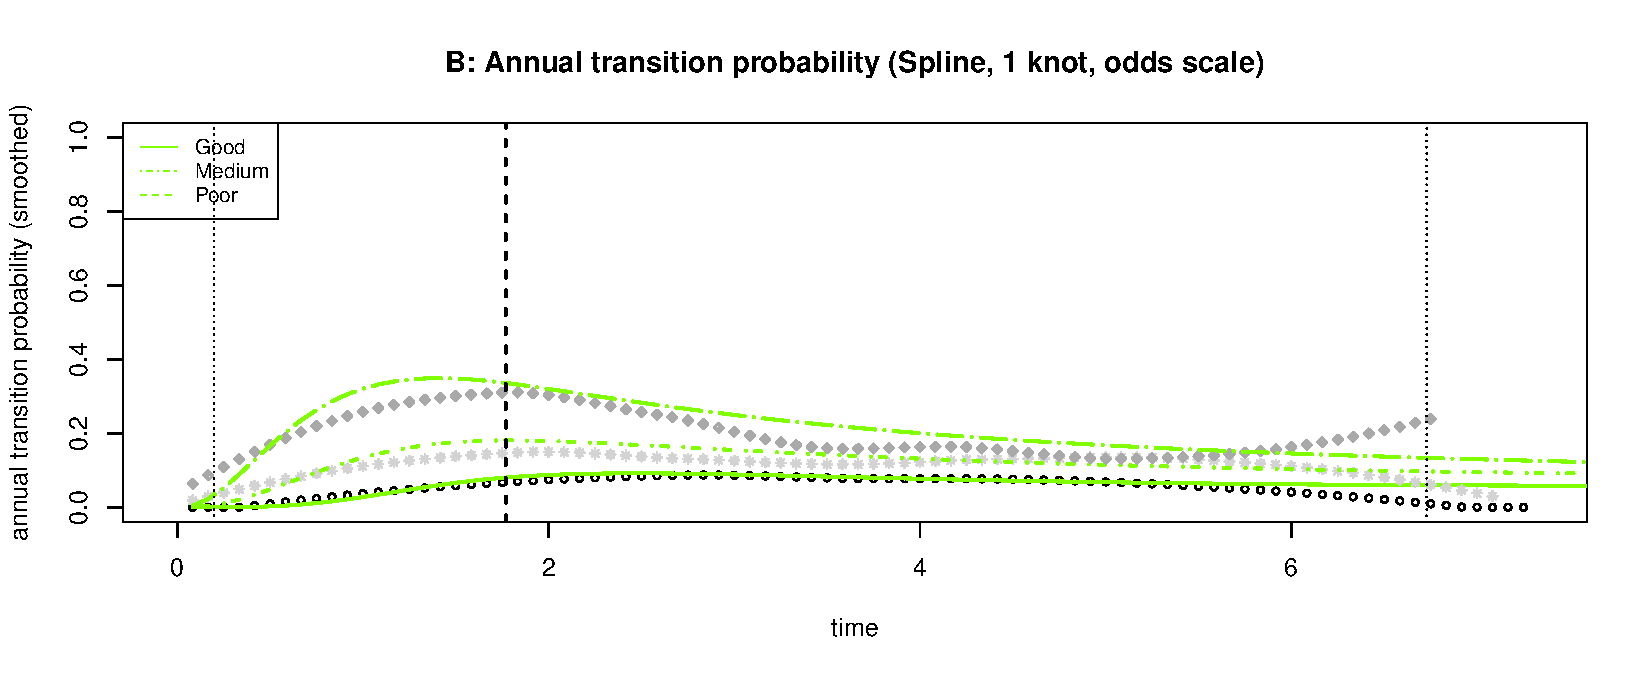
\includegraphics[height=0.3\textheight]{images/spline_odds1-2} \end{flushleft}

\begin{flushleft}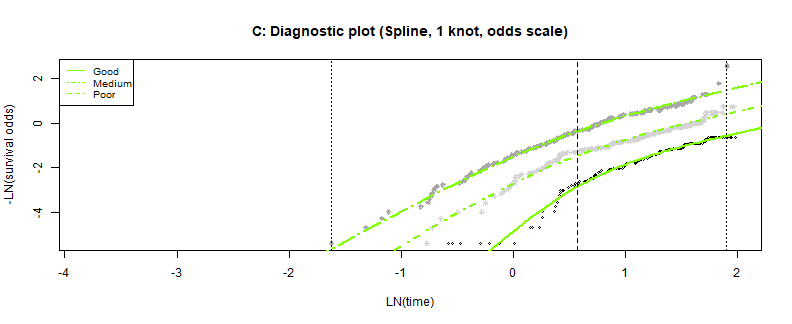
\includegraphics[height=0.3\textheight]{images/spline_odds1-3} \end{flushleft}

\subsection{Spline odds 2 knots}\label{spline-odds-2-knots}

\begin{flushleft}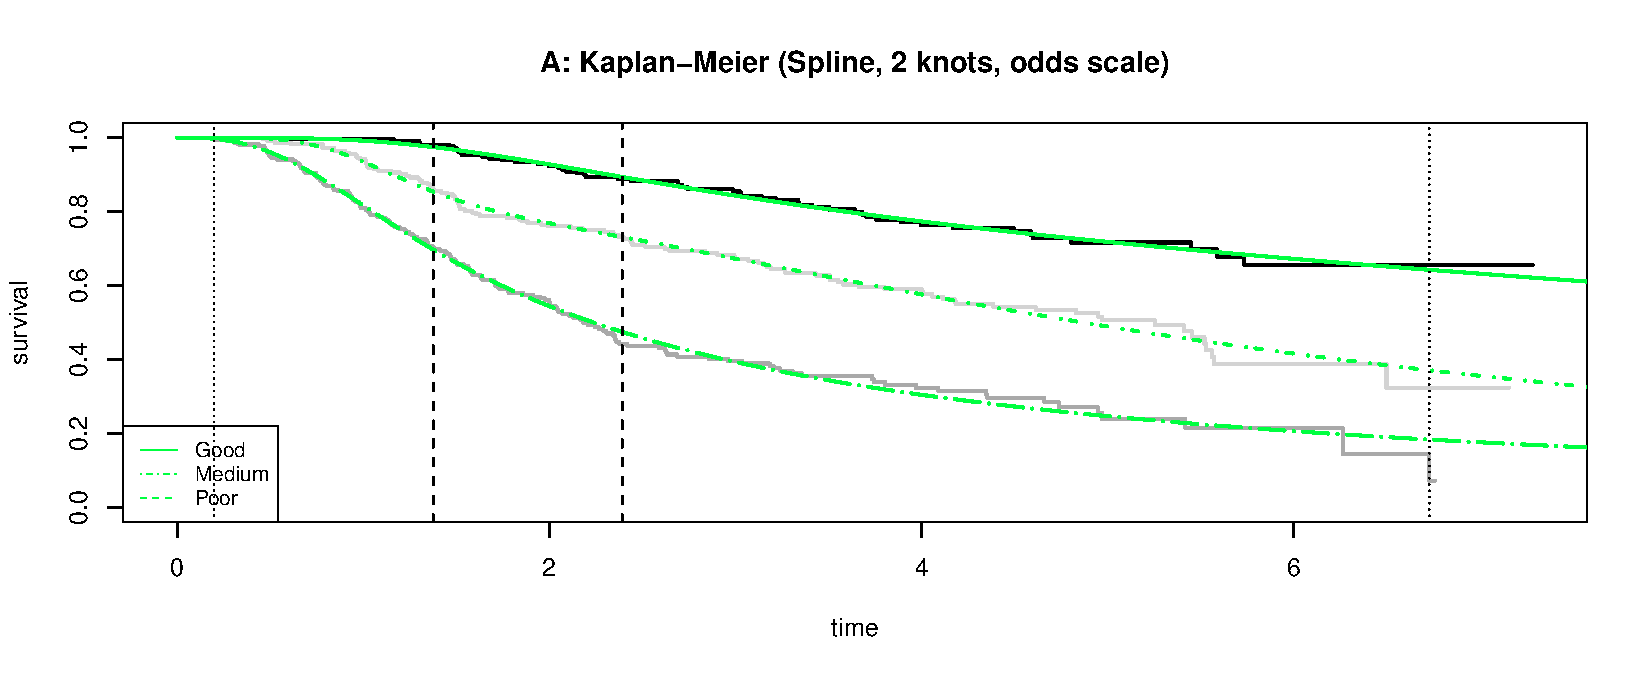
\includegraphics[height=0.3\textheight]{images/spline_odds2-1} \end{flushleft}

\begin{flushleft}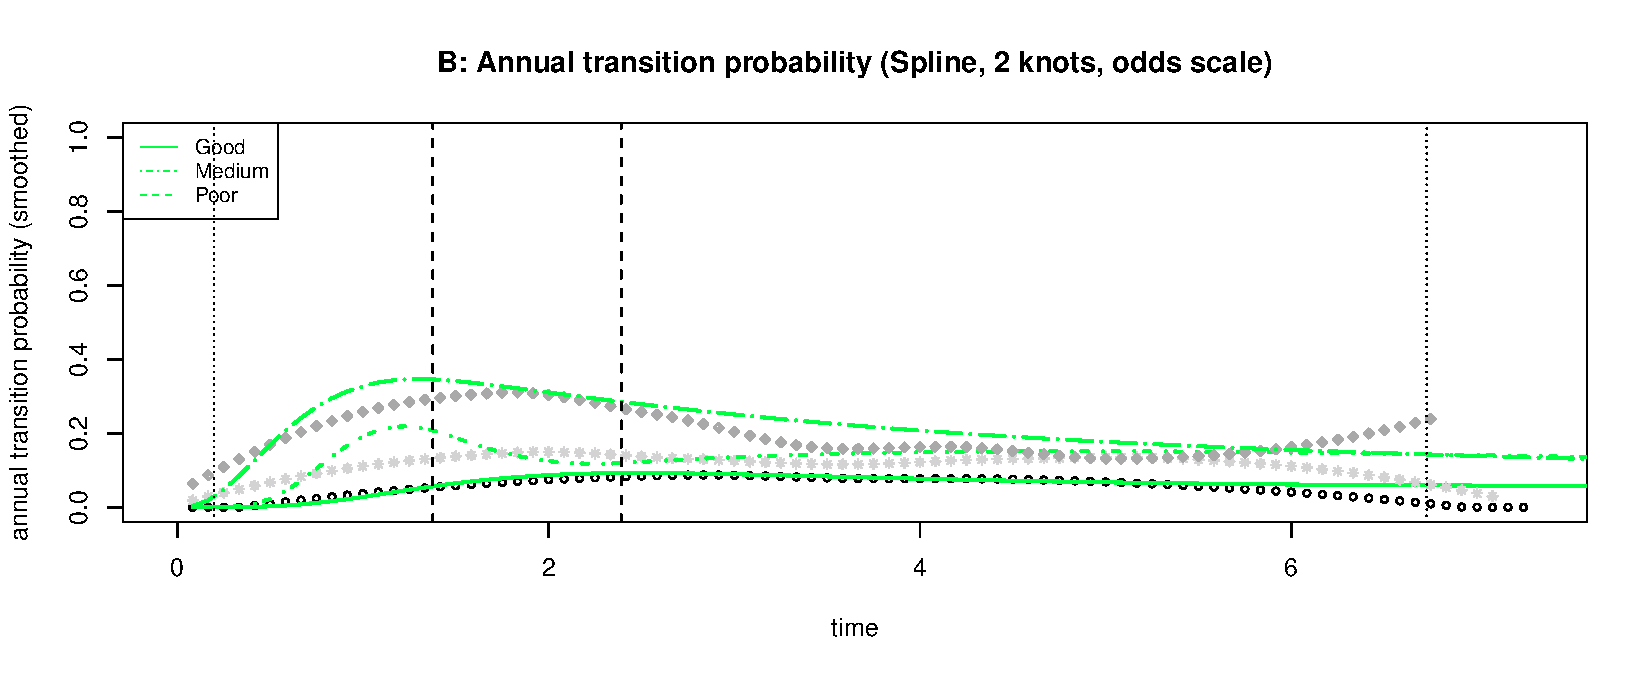
\includegraphics[height=0.3\textheight]{images/spline_odds2-2} \end{flushleft}

\begin{flushleft}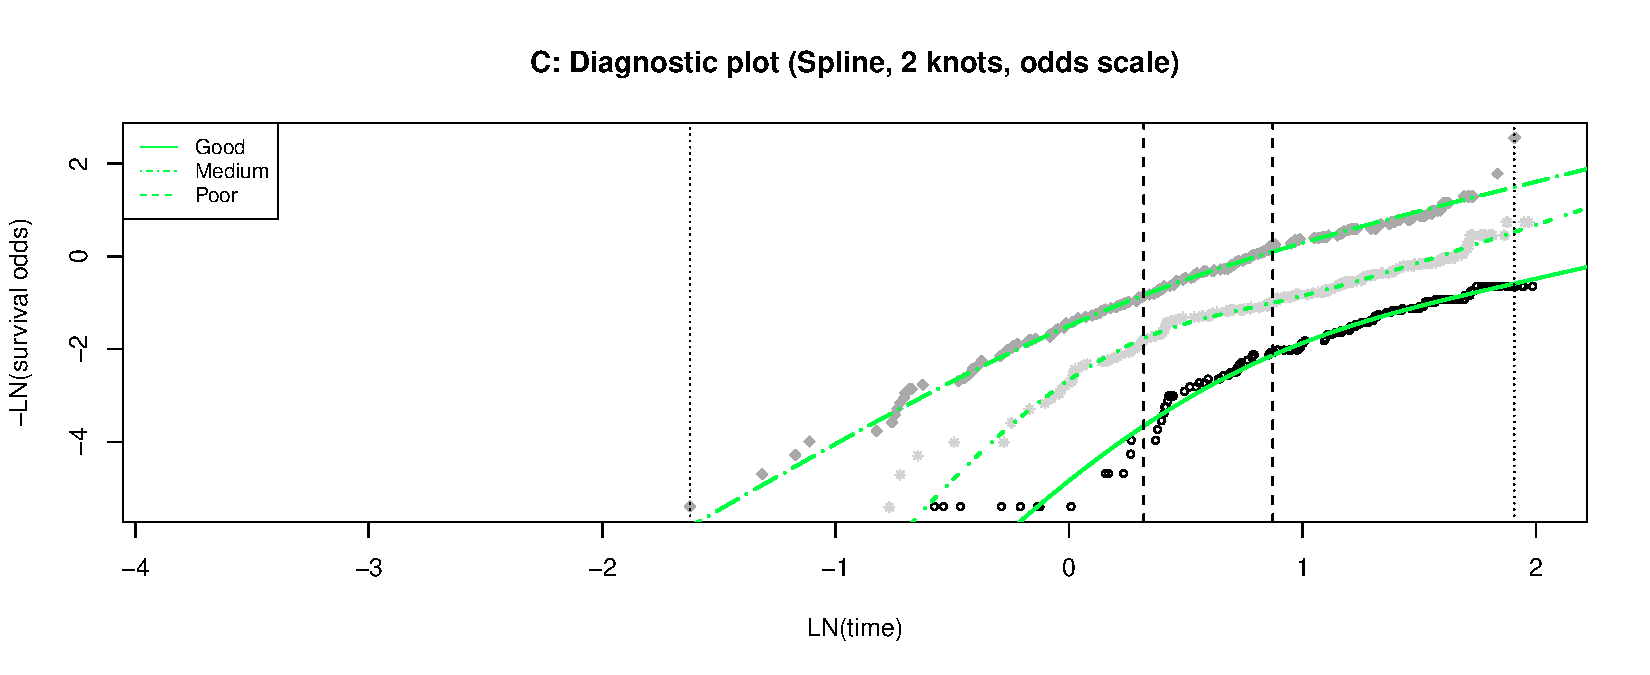
\includegraphics[height=0.3\textheight]{images/spline_odds2-3} \end{flushleft}

\subsection{Spline normal 1 knot}\label{spline-normal-1-knot}

\begin{flushleft}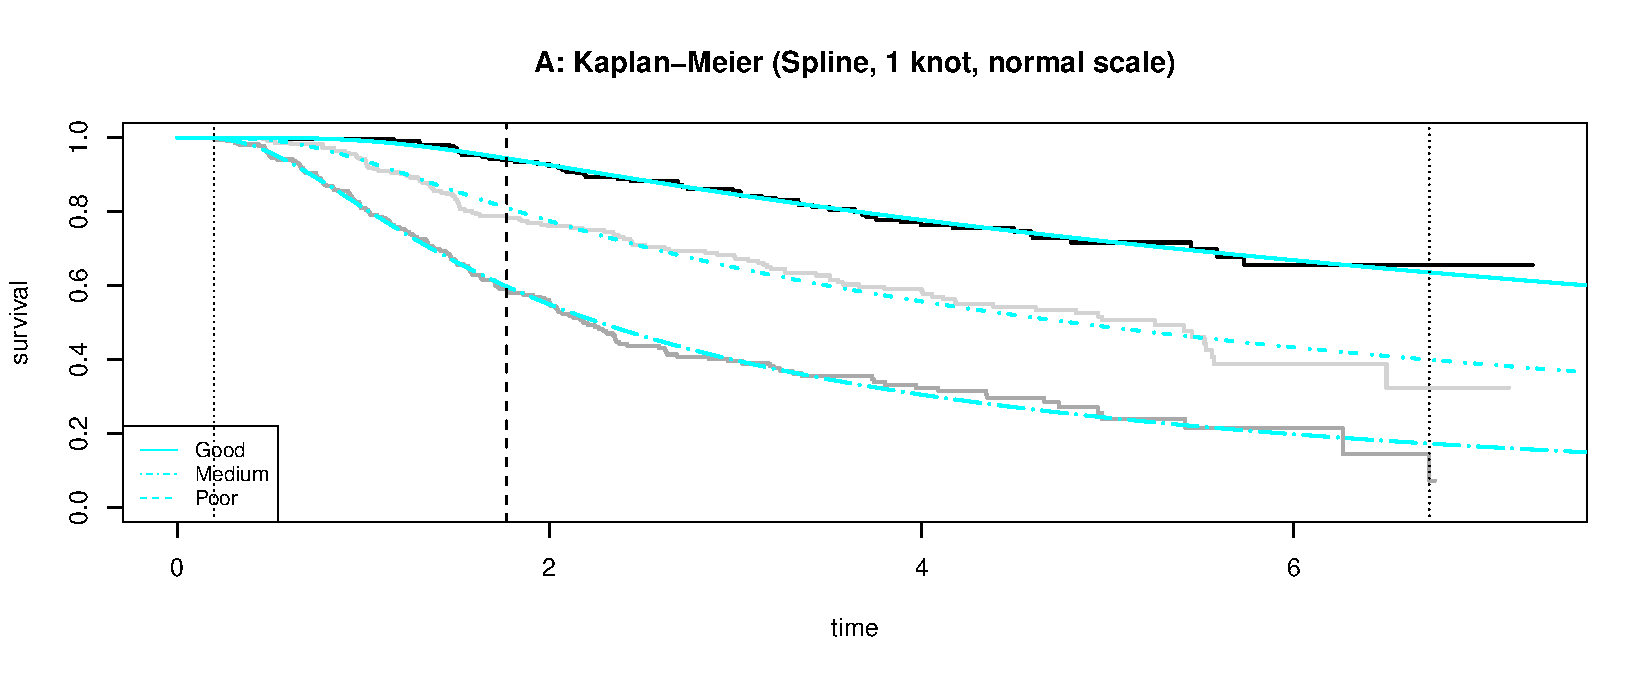
\includegraphics[height=0.3\textheight]{images/spline_norm1-1} \end{flushleft}

\begin{flushleft}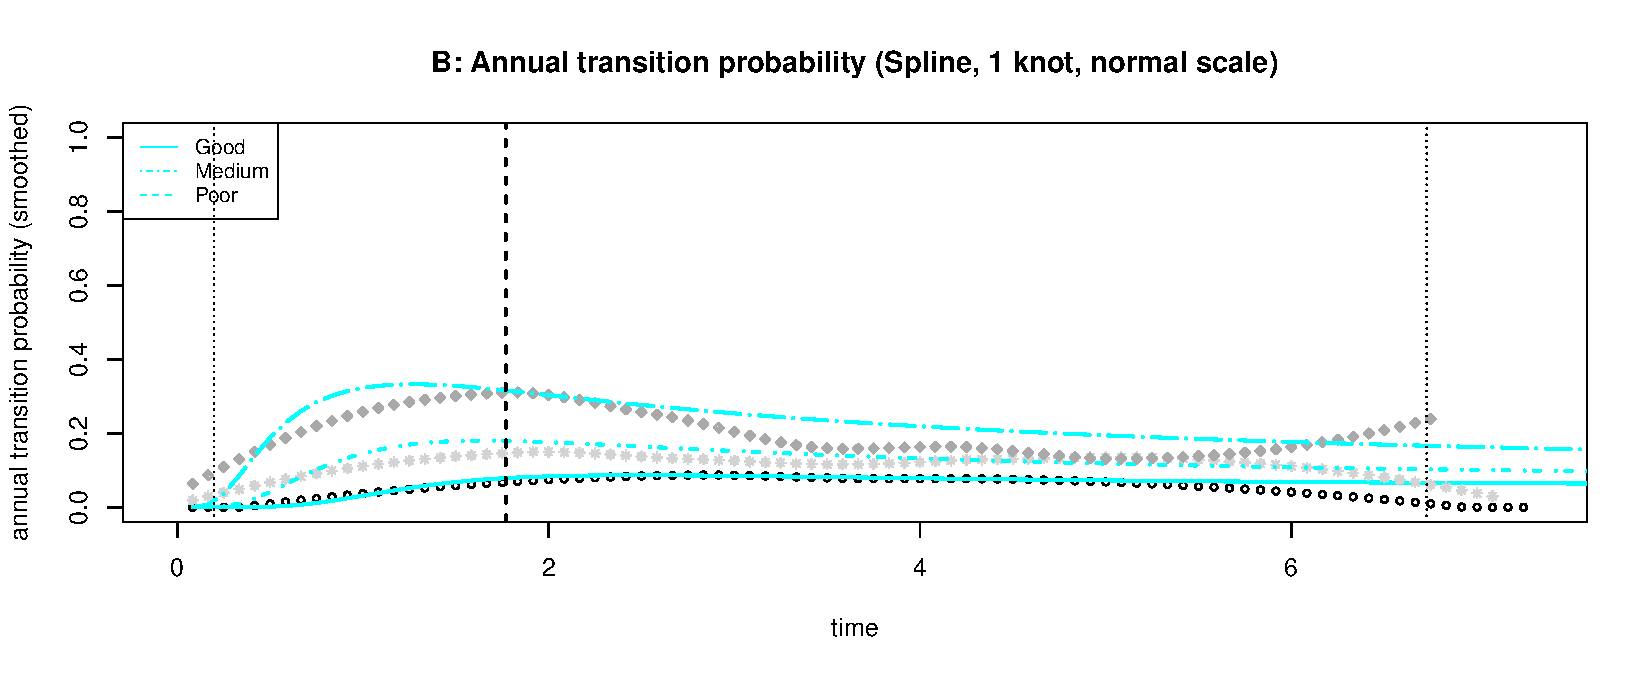
\includegraphics[height=0.3\textheight]{images/spline_norm1-2} \end{flushleft}

\begin{flushleft}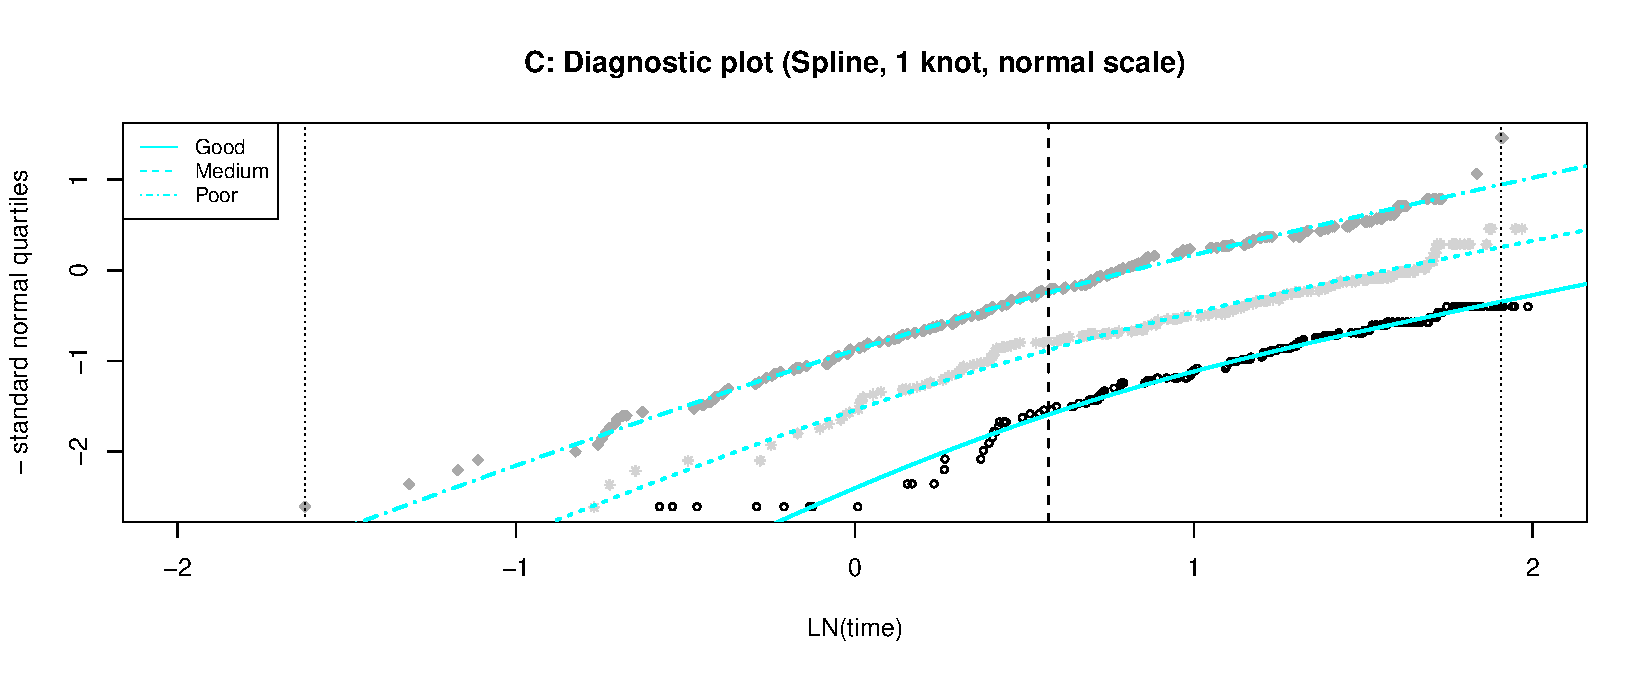
\includegraphics[height=0.3\textheight]{images/spline_norm1-3} \end{flushleft}

\subsection{Spline normal 2 knots}\label{spline-normal-2-knots}

\begin{flushleft}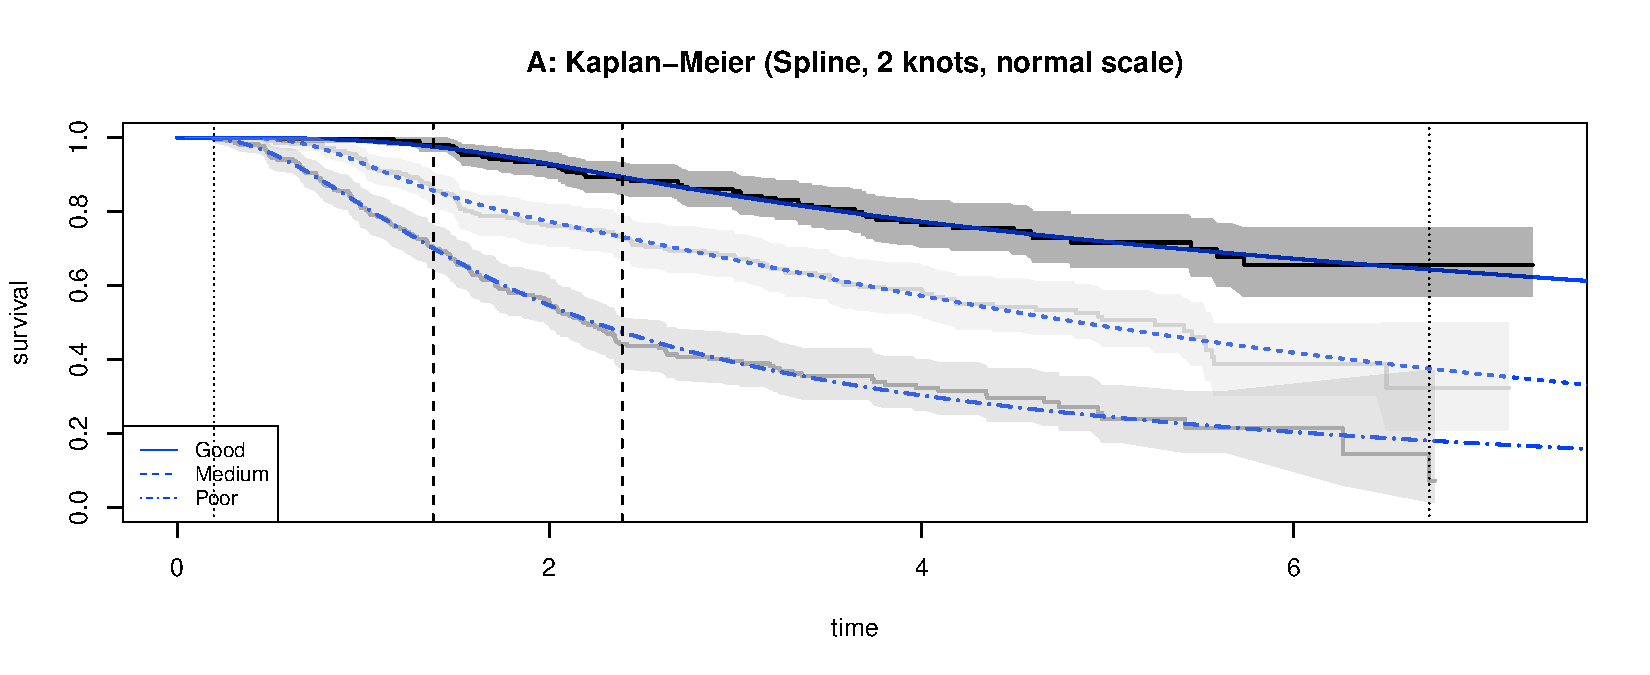
\includegraphics[height=0.3\textheight]{images/spline_norm2-1} \end{flushleft}

\begin{flushleft}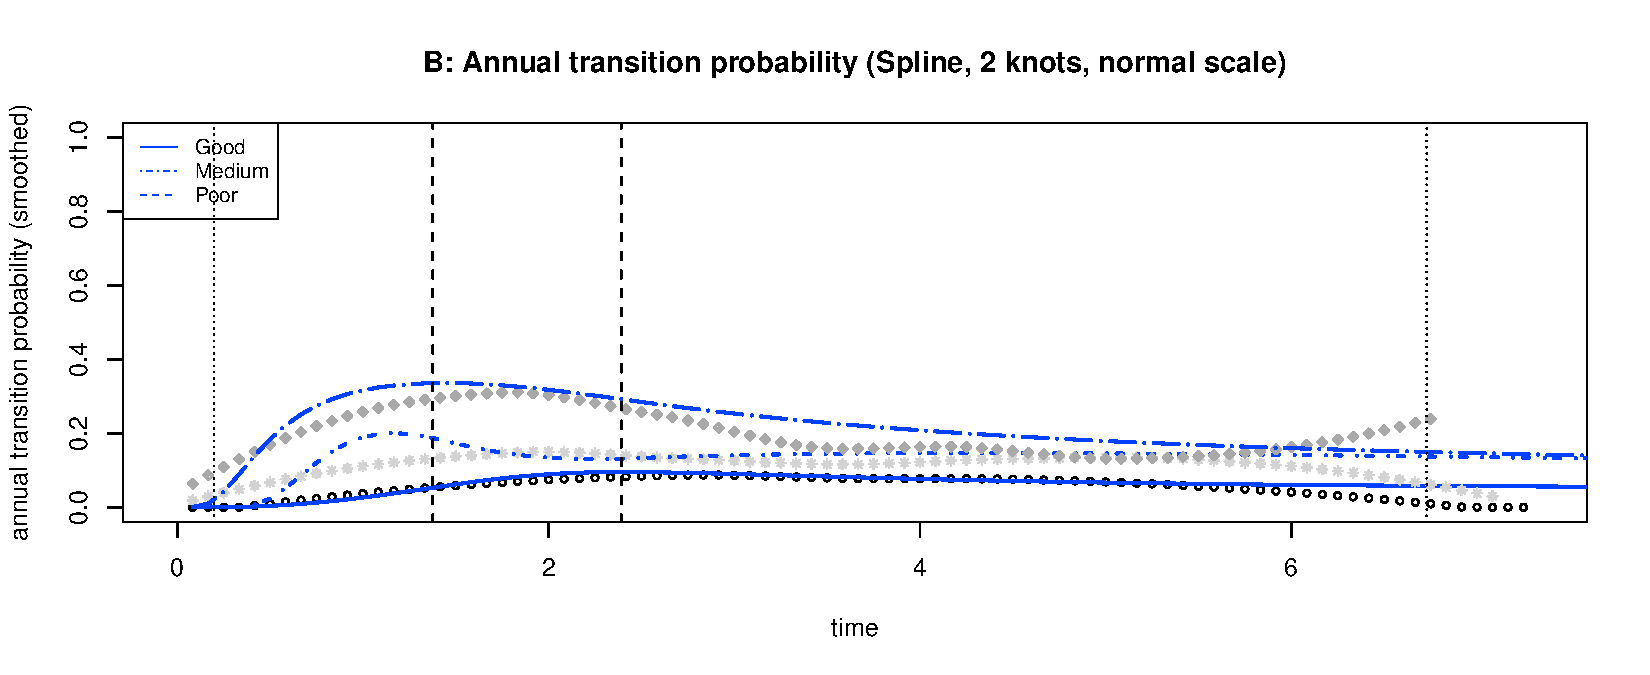
\includegraphics[height=0.3\textheight]{images/spline_norm2-2} \end{flushleft}

\begin{flushleft}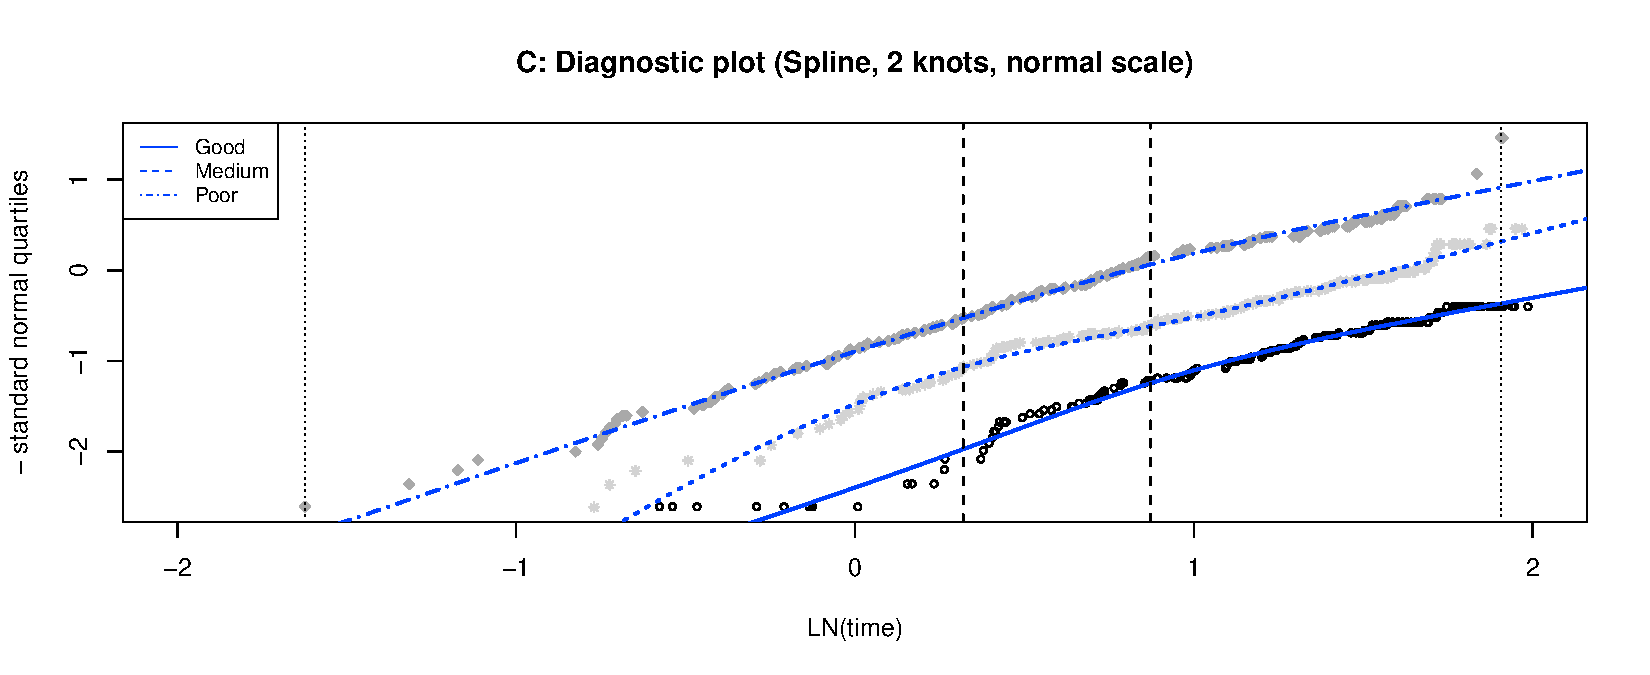
\includegraphics[height=0.3\textheight]{images/spline_norm2-3} \end{flushleft}

\newpage

\section{Validity of long-term
extrapolation?}\label{validity-of-long-term-extrapolation}

What model(s) is/are more appropriate for long-term extrapolation?
Are/is the selected model(s) plausible in comparison with general
population mortality?

\subsection{Group Good}\label{group-good}

\begin{flushleft}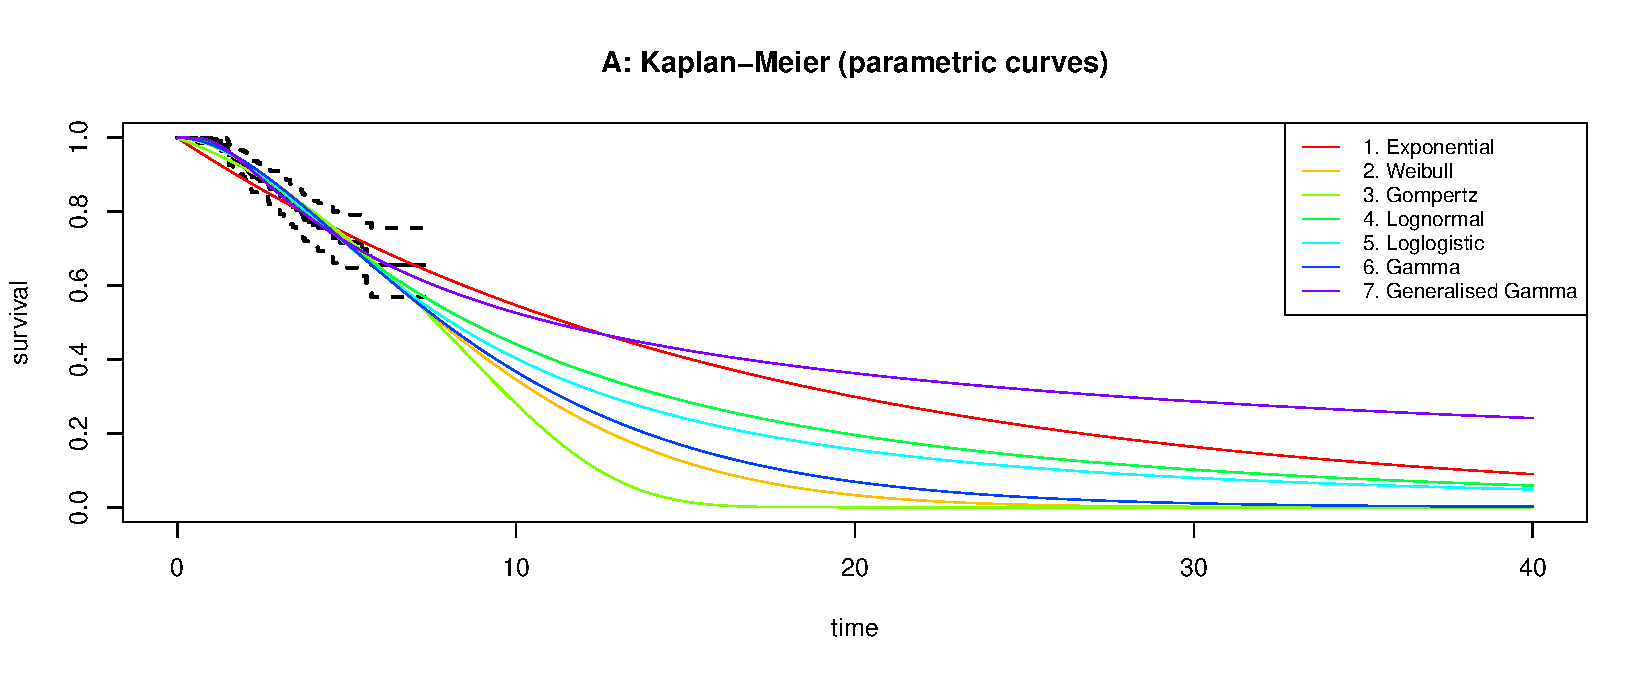
\includegraphics[height=0.29\textheight]{images/validate_extrapolation1-1} \end{flushleft}

\begin{flushleft}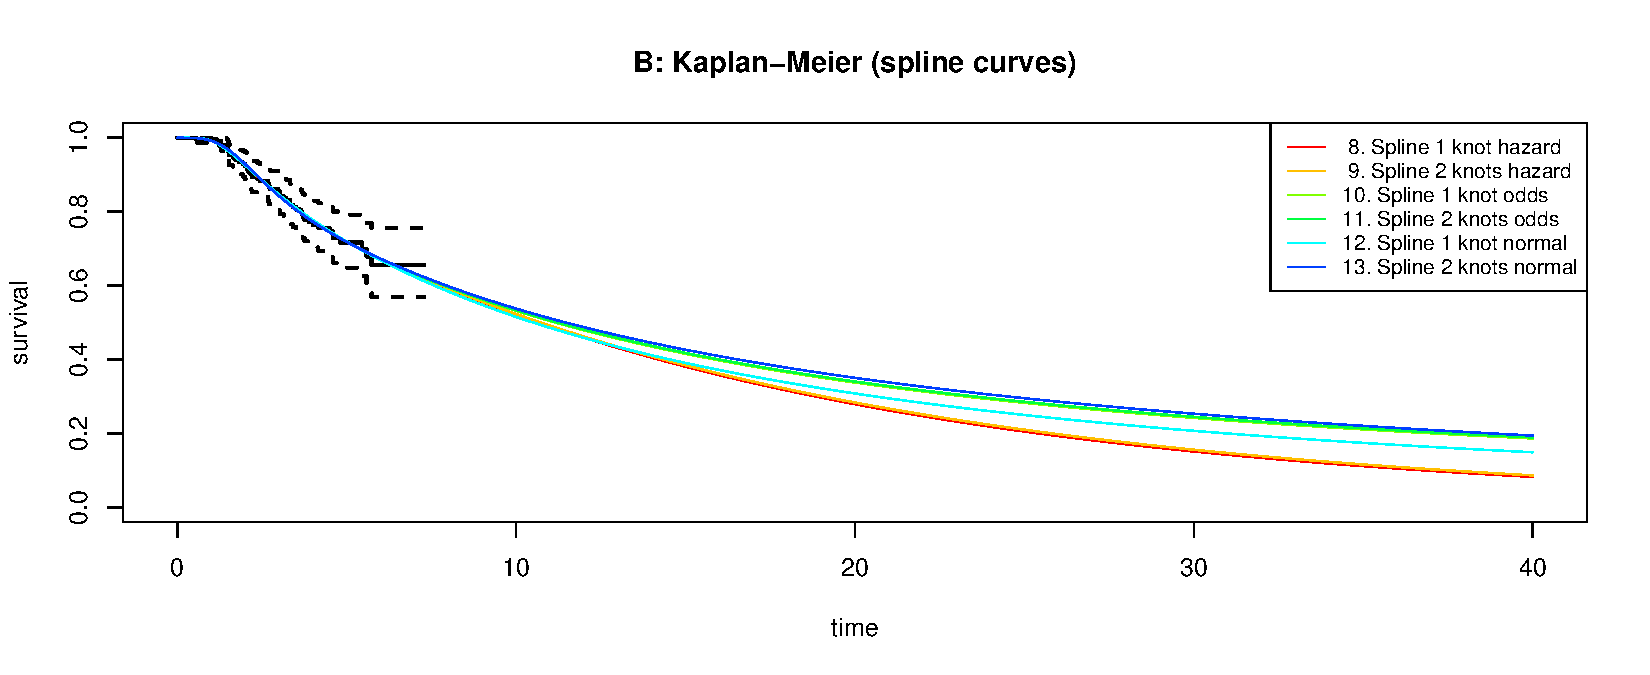
\includegraphics[height=0.29\textheight]{images/validate_extrapolation1-2} \end{flushleft}

\resizebox{\linewidth}{!}{
\begin{tabular}{lrrrrrrrrrrrr}
\toprule
  & T= 0 & T= 1 & T= 2 & T= 3 & T= 4 & T= 5 & T= 10 & T= 15 & T= 20 & T= 25 & T= 30 & T= 35\\
\midrule
\rowcolor{gray!6}  1. Exponential & 1 & 0.941 & 0.886 & 0.834 & 0.785 & 0.739 & 0.547 & 0.404 & 0.299 & 0.221 & 0.163 & 0.121\\
2. Weibull & 1 & 0.978 & 0.932 & 0.870 & 0.797 & 0.719 & 0.345 & 0.122 & 0.033 & 0.007 & 0.001 & 0.000\\
\rowcolor{gray!6}  3. Gompertz & 1 & 0.962 & 0.917 & 0.863 & 0.801 & 0.729 & 0.280 & 0.015 & 0.000 & 0.000 & 0.000 & 0.000\\
4. Log-normal & 1 & 0.986 & 0.933 & 0.861 & 0.785 & 0.713 & 0.441 & 0.287 & 0.196 & 0.139 & 0.102 & 0.076\\
\rowcolor{gray!6}  5. Log-logistic & 1 & 0.980 & 0.932 & 0.865 & 0.789 & 0.712 & 0.403 & 0.240 & 0.156 & 0.108 & 0.080 & 0.061\\
6. Gamma & 1 & 0.982 & 0.935 & 0.869 & 0.793 & 0.714 & 0.367 & 0.165 & 0.069 & 0.027 & 0.011 & 0.004\\
\rowcolor{gray!6}  7. Generalised Gamma & 1 & 0.991 & 0.928 & 0.849 & 0.778 & 0.717 & 0.526 & 0.425 & 0.362 & 0.319 & 0.286 & 0.261\\
8. Spline 1 knot hazard & 1 & 0.992 & 0.927 & 0.843 & 0.774 & 0.719 & 0.521 & 0.381 & 0.279 & 0.205 & 0.151 & 0.111\\
\rowcolor{gray!6}  9. Spline 2 knots hazard & 1 & 0.992 & 0.928 & 0.843 & 0.774 & 0.719 & 0.523 & 0.384 & 0.283 & 0.210 & 0.156 & 0.116\\
10. Spline 1 knot odds & 1 & 0.992 & 0.927 & 0.843 & 0.774 & 0.718 & 0.532 & 0.415 & 0.338 & 0.283 & 0.242 & 0.211\\
\rowcolor{gray!6}  11. Spline 2 knots odds & 1 & 0.992 & 0.928 & 0.843 & 0.774 & 0.718 & 0.533 & 0.418 & 0.340 & 0.285 & 0.245 & 0.213\\
12. Spline 1 knot normal & 1 & 0.992 & 0.926 & 0.847 & 0.778 & 0.719 & 0.515 & 0.391 & 0.308 & 0.250 & 0.207 & 0.174\\
\rowcolor{gray!6}  13. Spline 2 knots normal & 1 & 0.992 & 0.929 & 0.842 & 0.773 & 0.718 & 0.538 & 0.426 & 0.350 & 0.295 & 0.253 & 0.220\\
\bottomrule
\end{tabular}}

\begin{flushleft}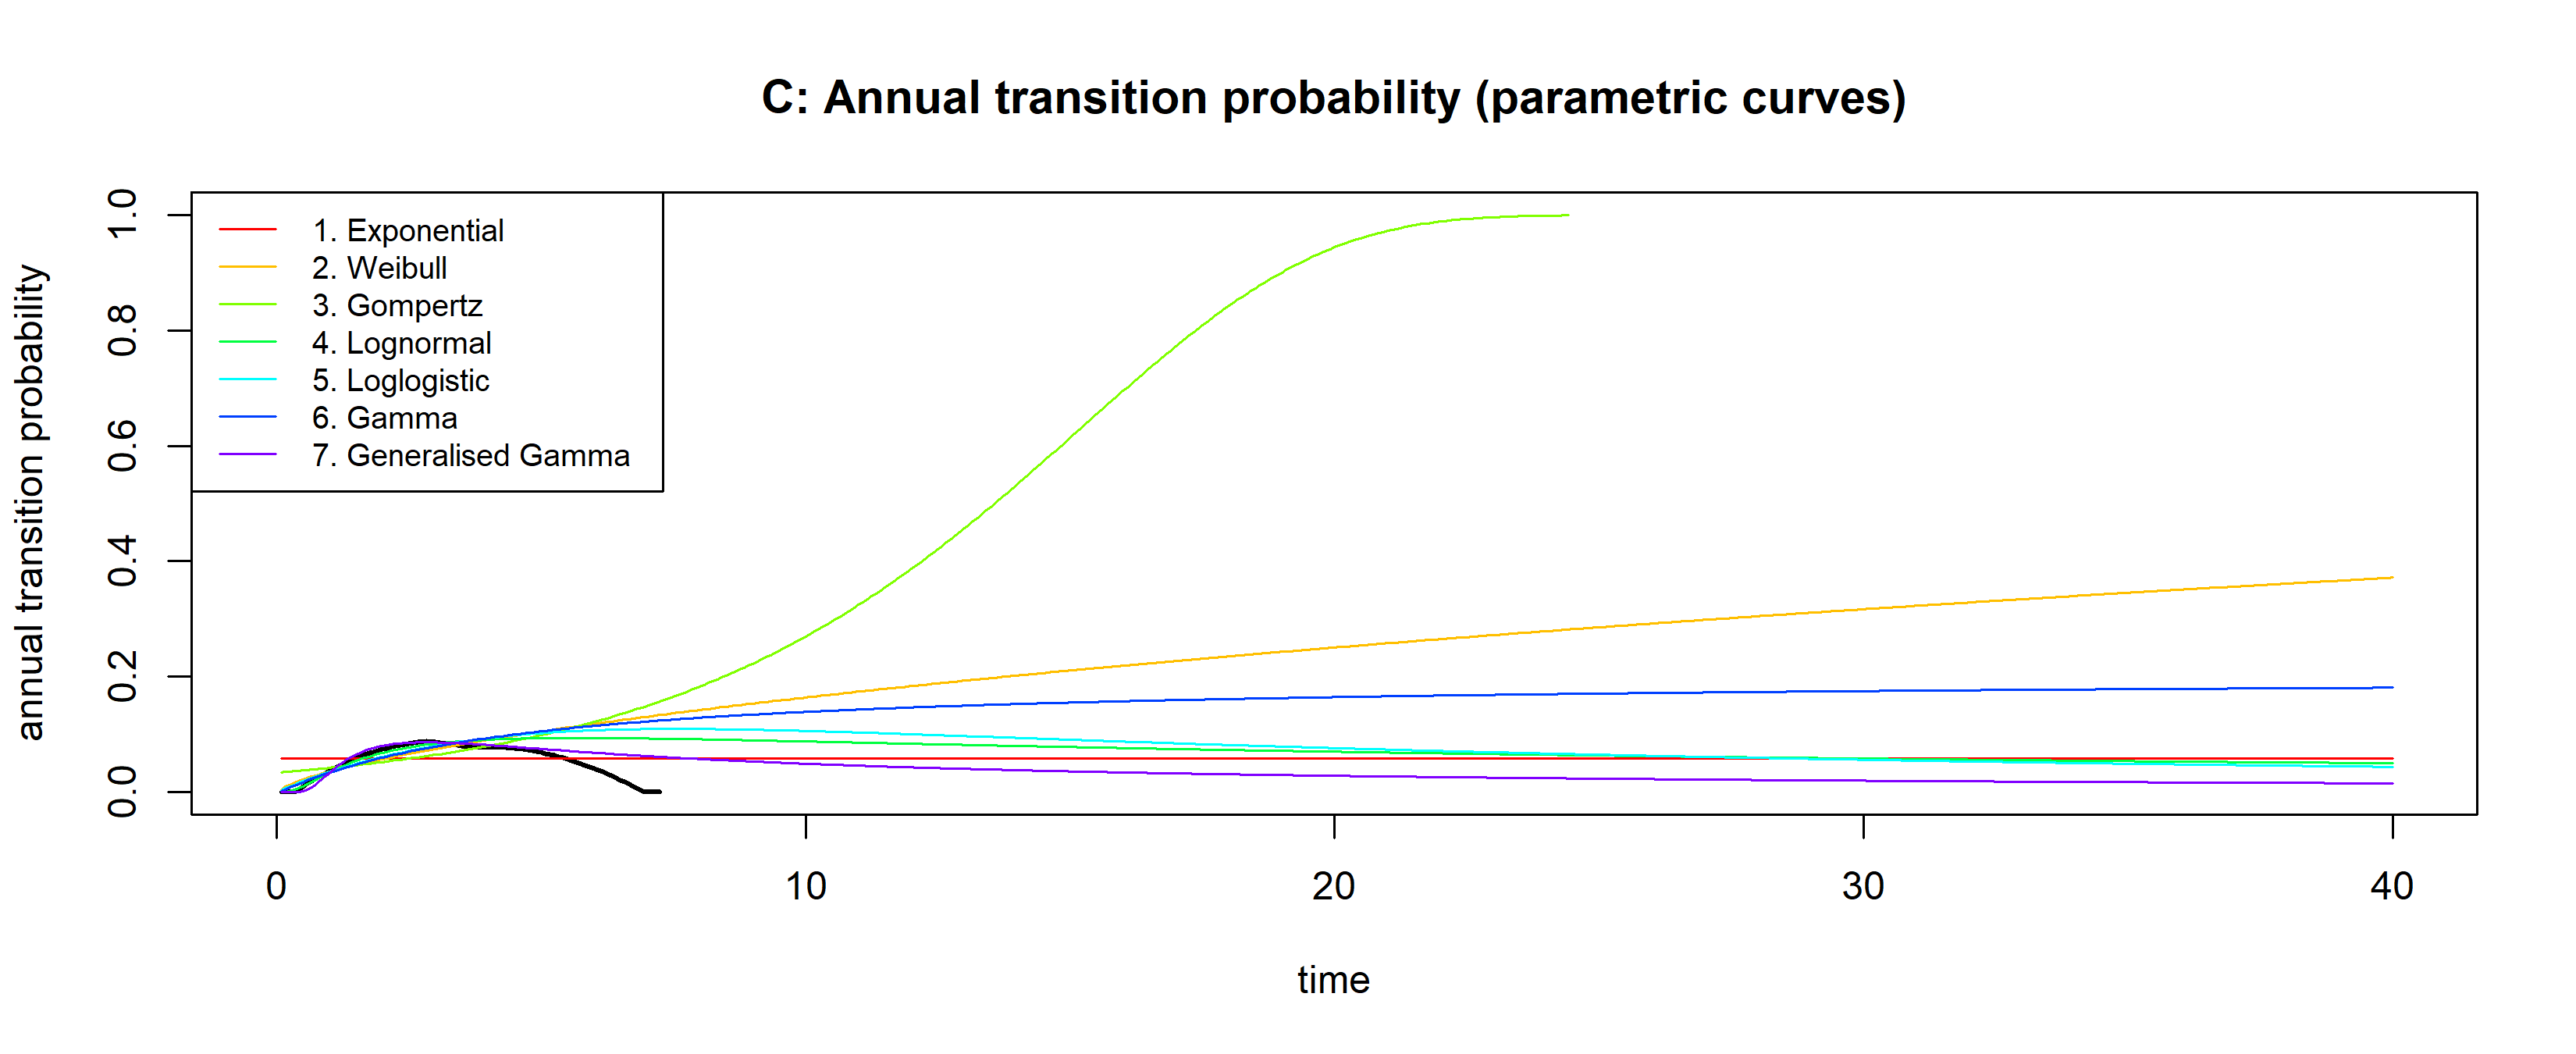
\includegraphics[height=0.29\textheight]{images/validate_extrapolation1-3} \end{flushleft}

\begin{flushleft}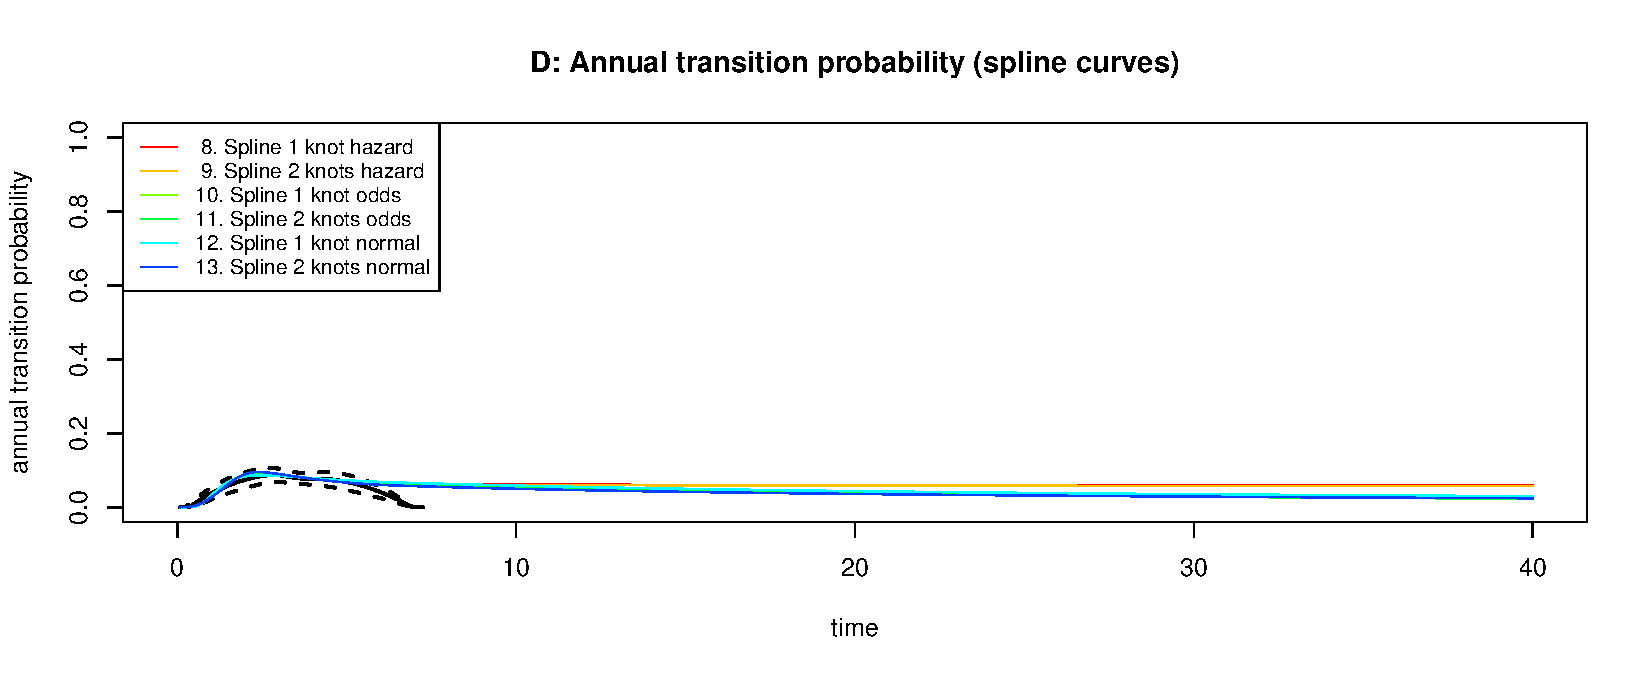
\includegraphics[height=0.29\textheight]{images/validate_extrapolation1-4} \end{flushleft}

\begin{tabular}{lrrrrr}
\toprule
  & Min & Q1 & Median & Q3 & Max\\
\midrule
\rowcolor{gray!6}  1. Exponential & 0.0585969 & 0.0585969 & 0.0585969 & 0.0585969 & 0.0585969\\
2. Weibull & 0.0039603 & 0.1641779 & 0.2507544 & 0.3170901 & 0.3714738\\
\rowcolor{gray!6}  3. Gompertz & 0.0342601 & 0.1256322 & 0.4037134 & 0.8634656 & 1.0000000\\
4. Log-normal & 0.0000121 & 0.0563972 & 0.0670524 & 0.0819079 & 0.0936091\\
\rowcolor{gray!6}  5. Log-logistic & 0.0022936 & 0.0533146 & 0.0700441 & 0.0935993 & 0.1092616\\
6. Gamma & 0.0014181 & 0.1390361 & 0.1644882 & 0.1750195 & 0.1807519\\
\rowcolor{gray!6}  7. Generalised Gamma & 0.0000000 & 0.0191123 & 0.0269247 & 0.0452063 & 0.0862100\\
8. Spline 1 knot hazard & 0.0000002 & 0.0592140 & 0.0598953 & 0.0610195 & 0.0916043\\
\rowcolor{gray!6}  9. Spline 2 knots hazard & 0.0000002 & 0.0576502 & 0.0585313 & 0.0599923 & 0.0923962\\
10. Spline 1 knot odds & 0.0000002 & 0.0281269 & 0.0363823 & 0.0502992 & 0.0917044\\
\rowcolor{gray!6}  11. Spline 2 knots odds & 0.0000002 & 0.0278516 & 0.0359503 & 0.0497462 & 0.0924439\\
12. Spline 1 knot normal & 0.0000000 & 0.0345970 & 0.0424046 & 0.0560095 & 0.0865141\\
\rowcolor{gray!6}  13. Spline 2 knots normal & 0.0000006 & 0.0281480 & 0.0348987 & 0.0473455 & 0.0953359\\
\bottomrule
\end{tabular}

\newpage

\subsection{Group Medium}\label{group-medium}

\begin{flushleft}\includegraphics[height=0.29\textheight]{images/validate_extrapolation2-1} \end{flushleft}

\begin{flushleft}\includegraphics[height=0.29\textheight]{images/validate_extrapolation2-2} \end{flushleft}

\resizebox{\linewidth}{!}{
\begin{tabular}{lrrrrrrrrrrrr}
\toprule
  & T= 0 & T= 1 & T= 2 & T= 3 & T= 4 & T= 5 & T= 10 & T= 15 & T= 20 & T= 25 & T= 30 & T= 35\\
\midrule
\rowcolor{gray!6}  1. Exponential & 1 & 0.872 & 0.761 & 0.663 & 0.578 & 0.505 & 0.255 & 0.128 & 0.065 & 0.033 & 0.016 & 0.008\\
2. Weibull & 1 & 0.923 & 0.811 & 0.693 & 0.578 & 0.474 & 0.141 & 0.032 & 0.006 & 0.001 & 0.000 & 0.000\\
\rowcolor{gray!6}  3. Gompertz & 1 & 0.898 & 0.794 & 0.689 & 0.586 & 0.486 & 0.117 & 0.007 & 0.000 & 0.000 & 0.000 & 0.000\\
4. Log-normal & 1 & 0.935 & 0.797 & 0.668 & 0.560 & 0.473 & 0.228 & 0.126 & 0.077 & 0.050 & 0.034 & 0.024\\
\rowcolor{gray!6}  5. Log-logistic & 1 & 0.927 & 0.801 & 0.673 & 0.561 & 0.468 & 0.218 & 0.124 & 0.081 & 0.057 & 0.043 & 0.034\\
6. Gamma & 1 & 0.930 & 0.813 & 0.689 & 0.572 & 0.469 & 0.154 & 0.045 & 0.013 & 0.003 & 0.001 & 0.000\\
\rowcolor{gray!6}  7. Generalised Gamma & 1 & 0.937 & 0.774 & 0.648 & 0.556 & 0.488 & 0.310 & 0.232 & 0.187 & 0.158 & 0.138 & 0.122\\
8. Spline 1 knot hazard & 1 & 0.939 & 0.782 & 0.652 & 0.558 & 0.486 & 0.265 & 0.150 & 0.087 & 0.052 & 0.031 & 0.019\\
\rowcolor{gray!6}  9. Spline 2 knots hazard & 1 & 0.935 & 0.766 & 0.673 & 0.579 & 0.490 & 0.184 & 0.061 & 0.018 & 0.005 & 0.001 & 0.000\\
10. Spline 1 knot odds & 1 & 0.939 & 0.778 & 0.648 & 0.556 & 0.489 & 0.301 & 0.213 & 0.162 & 0.131 & 0.109 & 0.093\\
\rowcolor{gray!6}  11. Spline 2 knots odds & 1 & 0.935 & 0.769 & 0.673 & 0.576 & 0.489 & 0.235 & 0.136 & 0.089 & 0.063 & 0.048 & 0.037\\
12. Spline 1 knot normal & 1 & 0.938 & 0.775 & 0.648 & 0.557 & 0.488 & 0.290 & 0.195 & 0.141 & 0.107 & 0.084 & 0.067\\
\rowcolor{gray!6}  13. Spline 2 knots normal & 1 & 0.930 & 0.773 & 0.669 & 0.572 & 0.489 & 0.240 & 0.135 & 0.083 & 0.054 & 0.037 & 0.026\\
\bottomrule
\end{tabular}}

\begin{flushleft}\includegraphics[height=0.29\textheight]{images/validate_extrapolation2-3} \end{flushleft}

\begin{flushleft}\includegraphics[height=0.29\textheight]{images/validate_extrapolation2-4} \end{flushleft}

\begin{tabular}{lrrrrr}
\toprule
  & Min & Q1 & Median & Q3 & Max\\
\midrule
\rowcolor{gray!6}  1. Exponential & 0.1278820 & 0.1278820 & 0.1278820 & 0.1278820 & 0.1278820\\
2. Weibull & 0.0298491 & 0.2382194 & 0.2998675 & 0.3413164 & 0.3730304\\
\rowcolor{gray!6}  3. Gompertz & 0.0960264 & 0.2326209 & 0.5026105 & 0.8415103 & 1.0000000\\
4. Log-normal & 0.0004751 & 0.0692201 & 0.0864990 & 0.1175437 & 0.1630482\\
\rowcolor{gray!6}  5. Log-logistic & 0.0150627 & 0.0512119 & 0.0722192 & 0.1148301 & 0.1673124\\
6. Gamma & 0.0159374 & 0.2105278 & 0.2273428 & 0.2338793 & 0.2373538\\
\rowcolor{gray!6}  7. Generalised Gamma & 0.0000000 & 0.0249765 & 0.0361491 & 0.0643696 & 0.1783037\\
8. Spline 1 knot hazard & 0.0005533 & 0.0961200 & 0.1007177 & 0.1087714 & 0.1767370\\
\rowcolor{gray!6}  9. Spline 2 knots hazard & 0.0000006 & 0.1921569 & 0.2213494 & 0.2415978 & 0.2568265\\
10. Spline 1 knot odds & 0.0004610 & 0.0331955 & 0.0461415 & 0.0743721 & 0.1809477\\
\rowcolor{gray!6}  11. Spline 2 knots odds & 0.0000004 & 0.0500917 & 0.0706148 & 0.1135216 & 0.2192447\\
12. Spline 1 knot normal & 0.0000012 & 0.0444894 & 0.0569700 & 0.0823605 & 0.1804334\\
\rowcolor{gray!6}  13. Spline 2 knots normal & 0.0000000 & 0.0682231 & 0.0852159 & 0.1164045 & 0.2005479\\
\bottomrule
\end{tabular}

\newpage

\subsection{Group Poor}\label{group-poor}

\begin{flushleft}\includegraphics[height=0.29\textheight]{images/validate_extrapolation3-1} \end{flushleft}

\begin{flushleft}\includegraphics[height=0.29\textheight]{images/validate_extrapolation3-2} \end{flushleft}

\resizebox{\linewidth}{!}{
\begin{tabular}{lrrrrrrrrrrrr}
\toprule
  & T= 0 & T= 1 & T= 2 & T= 3 & T= 4 & T= 5 & T= 10 & T= 15 & T= 20 & T= 25 & T= 30 & T= 35\\
\midrule
\rowcolor{gray!6}  1. Exponential & 1 & 0.755 & 0.570 & 0.430 & 0.325 & 0.245 & 0.060 & 0.015 & 0.004 & 0.001 & 0.000 & 0.000\\
2. Weibull & 1 & 0.817 & 0.608 & 0.430 & 0.292 & 0.193 & 0.017 & 0.001 & 0.000 & 0.000 & 0.000 & 0.000\\
\rowcolor{gray!6}  3. Gompertz & 1 & 0.776 & 0.588 & 0.436 & 0.315 & 0.221 & 0.022 & 0.001 & 0.000 & 0.000 & 0.000 & 0.000\\
4. Log-normal & 1 & 0.820 & 0.572 & 0.401 & 0.289 & 0.214 & 0.063 & 0.025 & 0.012 & 0.006 & 0.004 & 0.002\\
\rowcolor{gray!6}  5. Log-logistic & 1 & 0.819 & 0.568 & 0.389 & 0.275 & 0.203 & 0.069 & 0.034 & 0.021 & 0.014 & 0.010 & 0.008\\
6. Gamma & 1 & 0.829 & 0.605 & 0.420 & 0.283 & 0.187 & 0.020 & 0.002 & 0.000 & 0.000 & 0.000 & 0.000\\
\rowcolor{gray!6}  7. Generalised Gamma & 1 & 0.810 & 0.555 & 0.399 & 0.302 & 0.237 & 0.100 & 0.057 & 0.037 & 0.026 & 0.019 & 0.015\\
8. Spline 1 knot hazard & 1 & 0.822 & 0.545 & 0.390 & 0.301 & 0.244 & 0.109 & 0.056 & 0.031 & 0.018 & 0.011 & 0.007\\
\rowcolor{gray!6}  9. Spline 2 knots hazard & 1 & 0.817 & 0.546 & 0.396 & 0.305 & 0.243 & 0.096 & 0.043 & 0.021 & 0.010 & 0.005 & 0.003\\
10. Spline 1 knot odds & 1 & 0.820 & 0.542 & 0.390 & 0.303 & 0.248 & 0.127 & 0.082 & 0.060 & 0.047 & 0.038 & 0.032\\
\rowcolor{gray!6}  11. Spline 2 knots odds & 1 & 0.817 & 0.544 & 0.393 & 0.304 & 0.246 & 0.120 & 0.075 & 0.054 & 0.041 & 0.033 & 0.027\\
12. Spline 1 knot normal & 1 & 0.811 & 0.549 & 0.398 & 0.305 & 0.242 & 0.102 & 0.054 & 0.033 & 0.021 & 0.015 & 0.011\\
\rowcolor{gray!6}  13. Spline 2 knots normal & 1 & 0.815 & 0.546 & 0.392 & 0.303 & 0.245 & 0.113 & 0.065 & 0.042 & 0.029 & 0.021 & 0.016\\
\bottomrule
\end{tabular}}

\begin{flushleft}\includegraphics[height=0.29\textheight]{images/validate_extrapolation3-3} \end{flushleft}

\begin{flushleft}\includegraphics[height=0.29\textheight]{images/validate_extrapolation3-4} \end{flushleft}

\begin{tabular}{lrrrrr}
\toprule
  & Min & Q1 & Median & Q3 & Max\\
\midrule
\rowcolor{gray!6}  1. Exponential & 0.2449482 & 0.2449482 & 0.2449482 & 0.2449482 & 0.2449482\\
2. Weibull & 0.0907442 & 0.4105709 & 0.4790585 & 0.5216195 & 0.5525972\\
\rowcolor{gray!6}  3. Gompertz & 0.2169796 & 0.3698466 & 0.5818235 & 0.8071868 & 1.0000000\\
4. Log-normal & 0.0022958 & 0.1000774 & 0.1279068 & 0.1841659 & 0.3070152\\
\rowcolor{gray!6}  5. Log-logistic & 0.0305143 & 0.0571627 & 0.0832145 & 0.1494462 & 0.3207417\\
6. Gamma & 0.0471845 & 0.3701940 & 0.3852535 & 0.3907371 & 0.3935697\\
\rowcolor{gray!6}  7. Generalised Gamma & 0.0000317 & 0.0518395 & 0.0728961 & 0.1237607 & 0.3222943\\
8. Spline 1 knot hazard & 0.0048605 & 0.0929348 & 0.1060806 & 0.1322263 & 0.3462113\\
\rowcolor{gray!6}  9. Spline 2 knots hazard & 0.0027621 & 0.1183362 & 0.1309295 & 0.1552006 & 0.3471134\\
10. Spline 1 knot odds & 0.0040186 & 0.0370407 & 0.0534928 & 0.0956147 & 0.3493116\\
\rowcolor{gray!6}  11. Spline 2 knots odds & 0.0029239 & 0.0397013 & 0.0573770 & 0.1025038 & 0.3469030\\
12. Spline 1 knot normal & 0.0001727 & 0.0667705 & 0.0870224 & 0.1315769 & 0.3327152\\
\rowcolor{gray!6}  13. Spline 2 knots normal & 0.0003302 & 0.0575542 & 0.0758377 & 0.1164719 & 0.3361441\\
\bottomrule
\end{tabular}

\newpage

\section{Session information}\label{session-information}

\begin{verbatim}
## R version 4.0.1 (2020-06-06)
## Platform: x86_64-w64-mingw32/x64 (64-bit)
## Running under: Windows 10 x64 (build 18362)
## 
## Matrix products: default
## 
## Random number generation:
##  RNG:     Mersenne-Twister 
##  Normal:  Inversion 
##  Sample:  Rejection 
##  
## attached base packages:
## [1] stats     graphics  grDevices utils     datasets  methods   base     
## 
## other attached packages:
##  [1] kableExtra_1.1.0   knitr_1.28         summarytools_0.9.6 data.table_1.12.8 
##  [5] survminer_0.4.7    ggpubr_0.3.0       muhaz_1.2.6.1      flexsurv_1.1.1    
##  [9] rms_6.0-0          SparseM_1.78       Hmisc_4.4-0        ggplot2_3.3.2     
## [13] Formula_1.2-3      survival_3.2-3     lattice_0.20-41   
## 
## loaded via a namespace (and not attached):
##   [1] TH.data_1.0-10      colorspace_1.4-1    ggsignif_0.6.0     
##   [4] pryr_0.1.4          ellipsis_0.3.1      rio_0.5.16         
##   [7] htmlTable_1.13.3    base64enc_0.1-3     rstudioapi_0.11    
##  [10] farver_2.0.3        MatrixModels_0.4-1  mvtnorm_1.1-1      
##  [13] lubridate_1.7.9     xml2_1.3.2          codetools_0.2-16   
##  [16] splines_4.0.1       broom_0.5.6         km.ci_0.5-2        
##  [19] cluster_2.1.0       png_0.1-7           readr_1.3.1        
##  [22] compiler_4.0.1      httr_1.4.1          backports_1.1.7    
##  [25] Matrix_1.2-18       acepack_1.4.1       htmltools_0.4.0    
##  [28] quantreg_5.55       tools_4.0.1         gtable_0.3.0       
##  [31] glue_1.4.1          dplyr_1.0.0         Rcpp_1.0.4.6       
##  [34] carData_3.0-4       cellranger_1.1.0    vctrs_0.3.0        
##  [37] nlme_3.1-148        xfun_0.14           stringr_1.4.0      
##  [40] openxlsx_4.1.5      rvest_0.3.5         lifecycle_0.2.0    
##  [43] rstatix_0.5.0       polspline_1.1.19    MASS_7.3-51.6      
##  [46] zoo_1.8-8           scales_1.1.1        hms_0.5.3          
##  [49] sandwich_2.5-1      RColorBrewer_1.1-2  yaml_2.2.1         
##  [52] curl_4.3            gridExtra_2.3       KMsurv_0.1-5       
##  [55] pander_0.6.3        rpart_4.1-15        latticeExtra_0.6-29
##  [58] stringi_1.4.6       checkmate_2.0.0     zip_2.0.4          
##  [61] rlang_0.4.6         pkgconfig_2.0.3     matrixStats_0.56.0 
##  [64] evaluate_0.14       purrr_0.3.4         rapportools_1.0    
##  [67] htmlwidgets_1.5.1   labeling_0.3        tidyselect_1.1.0   
##  [70] deSolve_1.28        plyr_1.8.6          magrittr_1.5       
##  [73] R6_2.4.1            magick_2.3          generics_0.0.2     
##  [76] multcomp_1.4-13     pillar_1.4.4        haven_2.3.1        
##  [79] foreign_0.8-80      withr_2.2.0         abind_1.4-5        
##  [82] nnet_7.3-14         tibble_3.0.1        mstate_0.2.12      
##  [85] crayon_1.3.4        car_3.0-8           survMisc_0.5.5     
##  [88] rmarkdown_2.2       jpeg_0.1-8.1        grid_4.0.1         
##  [91] readxl_1.3.1        forcats_0.5.0       digest_0.6.25      
##  [94] webshot_0.5.2       xtable_1.8-4        tidyr_1.1.0        
##  [97] munsell_0.5.0       viridisLite_0.3.0   tcltk_4.0.1        
## [100] quadprog_1.5-8
\end{verbatim}

\end{document}
